\documentclass[aip,reprint,nofootinbib]{revtex4-1}
%\documentclass[aip]{revtex4-1}

\usepackage[english]{babel}
\usepackage{amsmath,amssymb}
\usepackage{graphicx}% Include figure files
\usepackage{color}% Include colors for document elements
\usepackage{dcolumn}% Align table columns on decimal point
\newcolumntype{.}{D{.}{.}{-1}}  % Align table cell values by decimal point
\RequirePackage{chemfig} % diagrammes chimiques
%\setatomsep{50pt}
\RequirePackage{array}						%% amélioration des tableaux
\usepackage{makecell}
%\usepackage{refcheck} % chercher les citations pas utilisées

\renewcommand\theadalign{bc}
\renewcommand\theadfont{\bfseries}
\renewcommand\theadgape{\Gape[4pt]}
\renewcommand\cellgape{\Gape[4pt]}

\graphicspath{{./}{data/}{images/}{figures/}}

\makeatletter
% A change to a babel macro
\def\bbl@set@language#1{%
  \edef\languagename{%
    \ifnum\escapechar=\expandafter`\string#1\@empty
    \else\string#1\@empty\fi}%
  %%%% ADDITION
  \@ifundefined{babel@language@alias@\languagename}{}{%
    \edef\languagename{\@nameuse{babel@language@alias@\languagename}}%
  }%
  %%%% END ADDITION
  \select@language{\languagename}%
  \expandafter\ifx\csname date\languagename\endcsname\relax\else
    \if@filesw
      \protected@write\@auxout{}{\string\select@language{\languagename}}%
      \bbl@for\bbl@tempa\BabelContentsFiles{%
        \addtocontents{\bbl@tempa}{\xstring\select@language{\languagename}}}%
      \bbl@usehooks{write}{}%
    \fi
  \fi}
% The user interface
\newcommand{\DeclareLanguageAlias}[2]{%
  \global\@namedef{babel@language@alias@#1}{#2}%
}
\makeatother

\DeclareLanguageAlias{en}{english}

\begin{document}

\title{An Illustrious Title}
\author{Alexander Punter}
\author{Paola Nava}
\author{Yannick Carissan}
\affiliation{Aix Marseille Univ, CNRS, Centrale Marseille, iSm2, Marseille, France}

\maketitle

\section{Introduction}

A great introduction.

\section{Methodology}

\subsection{Pseudopotential Form}
\label{sec:pseudoform}

In most pseudopotential methods, the techniques have revolved around separating the electrons of an atom into core and valence electrons. We propose a different formulation. Our goal is to investigate the feasibility of pseudopotentials reproducing electronic behaviour accurately, having been designed not only to replace the core electrons of small molecular fragments, but also to replace specific valence electrons that do not take part in the electronic behaviour in which we are interested.

As in the previous work, we have decided to restrict ourselves to creating an `out of the box' method, where no modification of quantum chemistry package source code should be necessary. This was done so as to keep the potentials independent of the quantum chemistry package used. The main quantum chemistry package we use is Turbomole~\cite{TURBOMOLE}, meaning our potentials are of the form

\begin{equation}
\sum_{k}{A_k(r^{n_{k}-2})e^{-\alpha_{k}r^{2}}}
\label{eq:turbomoleecp}
\end{equation}

where $n_k$ is an integer and where the total number of expressions $k$ can run across multiple such expressions for each angular momentum $l$. This means that any such potentials can be described in pseudopotential terms as `semi-local', meaning that they have an angular momentum component, but that they are not expanded in the atomic Gaussian basis sets. Equation~\ref{eq:turbomoleecp} means we have a choice of three variables per potential function, $A_k$, $n_k$ and $\alpha_k$. Throughout this work, the value of $n_k$ is fixed at 1. We limit ourselves to a maximum of one potential function per angular momentum $l$ for each potential centre. This is done only for the sake of simplicity and the possiblity of increasing this limit is discussed in Section~\ref{sec:further_development}. There is however a precedent of the main group elements being sufficiently well-described by a single potential function per angular momentum~\cite{igelmann_1988}.

The next departure from most pseudopotential methods is that we remove whole atoms from the molecular fragments for which we create potentials, as well as some further protons (see REF). We instead use non-atom-centered potentials. In full then, the multi-centered pseudopotential operator can be written as

\begin{multline}
\label{eq:ourPP}
\hat{W} = \frac{A}{r}
\underbrace{\exp(-\alpha r^2)\sum_m\left|Y_{1,m}\right>\left<Y_{1,m}\right|}_{\text{atom-centered potentials}}%
\\ +
\underbrace{\sum_J\frac{C_J}{r-r^{0}_J}\exp(-\gamma_J (r-r^0_J)^2)\left|Y_{0,0}\right>\left<Y_{0,0}\right|}_{\text{non-atom-centered potentials}}
\end{multline}

with $Y_{0,0}$ the $s$ spherical harmonic, $Y_{1,m}$ the $p$ spherical harmonics and $r^0_J$ the relative fixed position of the $J^{th}$ potential with respect to the origin of the pseudoatom to which the potentials are assigned. This $\hat{W}$ operator can then be added to the mono-electronic operator

\begin{equation}
\label{eq:monoElectronicOperator2}
\hat{h}(i) = -\frac{1}{2}\Delta_i - \frac{1}{r_i} + \sum_{K}{\hat{W}_k}
\end{equation}

where $K$ is the number of pseudofragments.

\subsection{Pseuodpotential Setups}

In keeping with our philosophy described in Section~\ref{sec:pseudoform} of retaining only the chemically-relevant parts of the system, we designed three four potential set-ups that kept only the bonding atoms. These consisted of two for $sp^2$ carbon atoms, and two for $sp^3$ carbon atoms. These we termed $\alpha$, $\beta$, $\gamma$ and $\delta$ potentials respectively. All four set-ups are summarised in Table~\ref{tab:pseudodiags}.

\begin{table}[h]
\begin{center}
\caption[Summary of $\alpha$, $\beta$, $\gamma$ and $\delta$ potentials.]{A summary of different pseudopotential set-ups presented in this work. Non-atom-centered potentials are highlighted in red.}\label{tab:pseudodiags}
\begin{tabular}{|c|c|c|}
\hline
\textbf{Diagram} & \textbf{Designation} & \textbf{Description} \\
\hline
\raisebox{-.5\height}{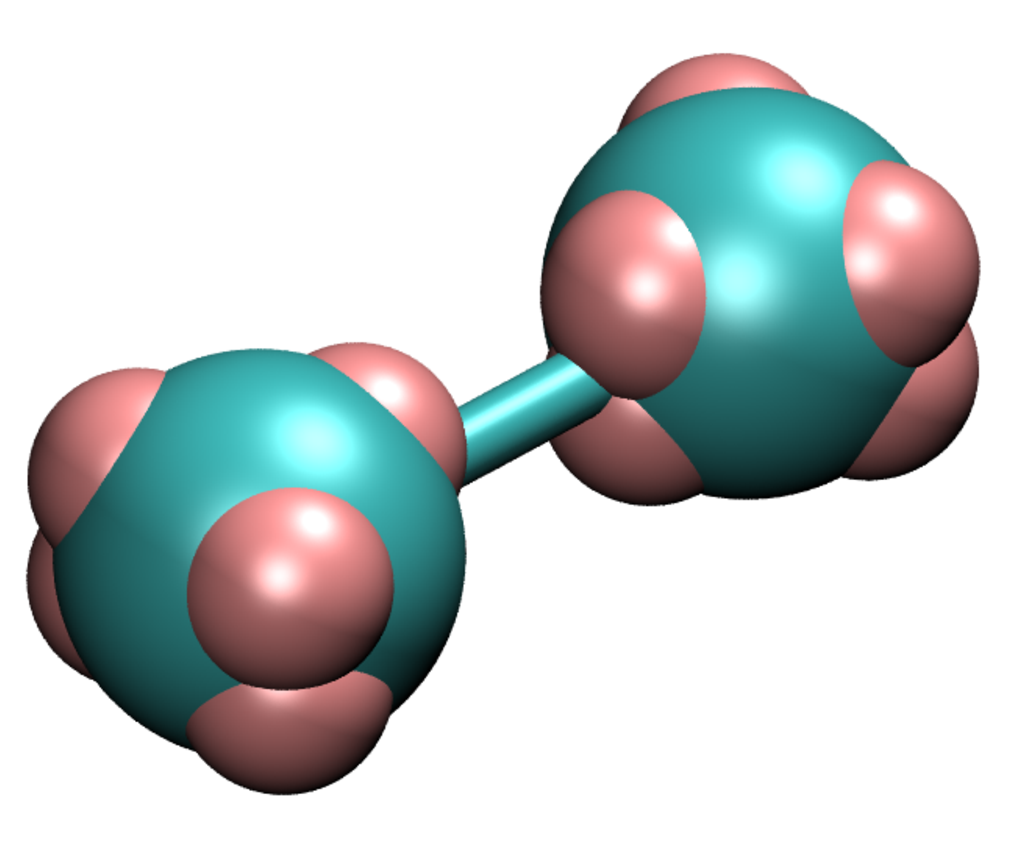
\includegraphics[width=2cm]{alpha}}
& $\alpha$ & $sp^2$ 1-electron\\
\hline
\raisebox{-.5\height}{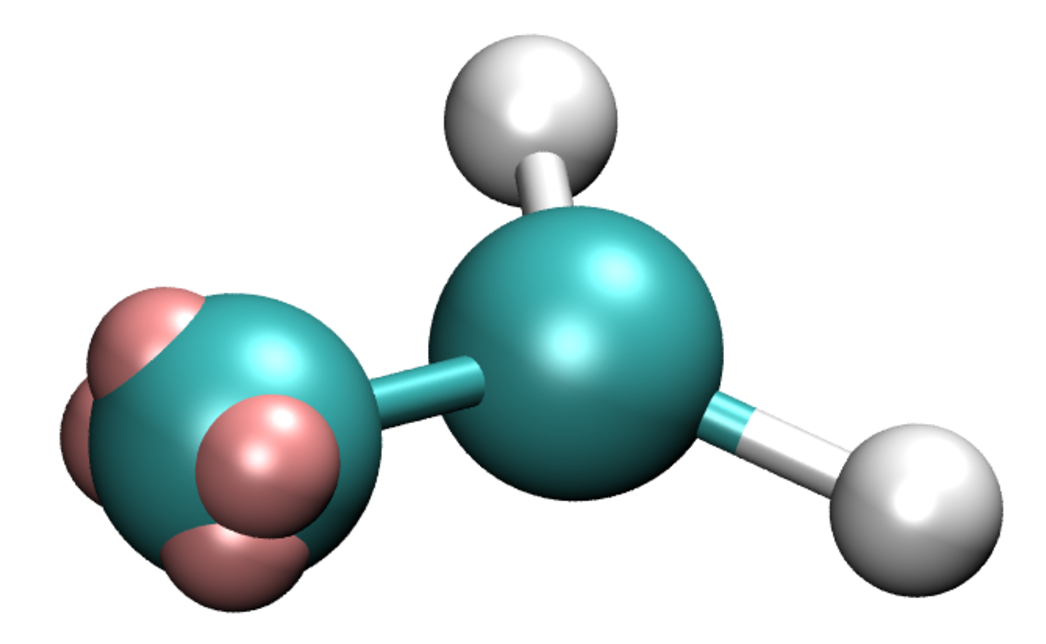
\includegraphics[width=2cm]{beta}}
& $\beta$ & $sp^2$ 1-electron \\
\hline
\raisebox{-.5\height}{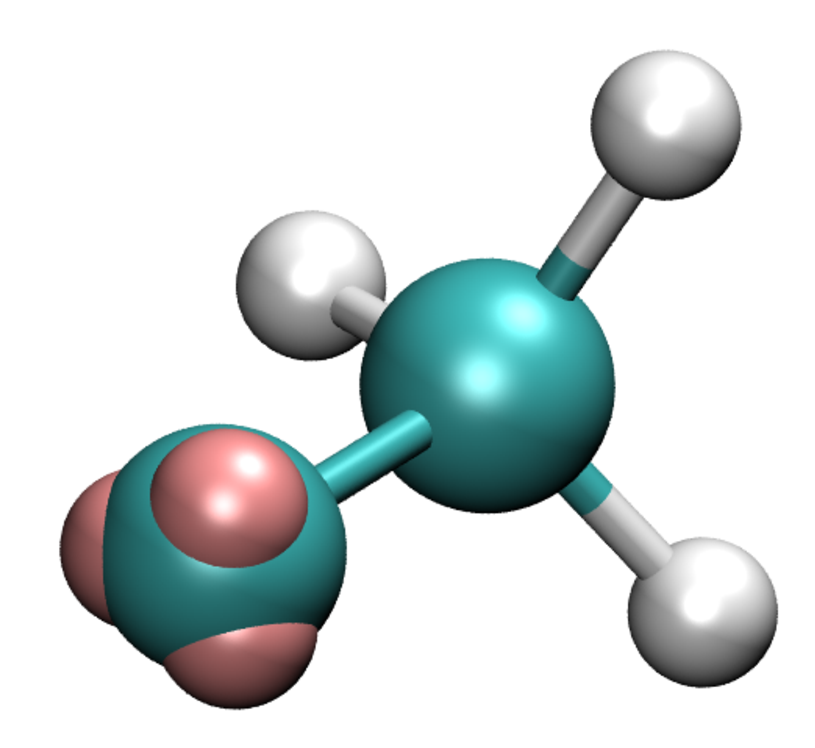
\includegraphics[width=2cm]{gamma}}
& $\gamma$ & $sp^3$ 2-electron \\
\hline
\raisebox{-.5\height}{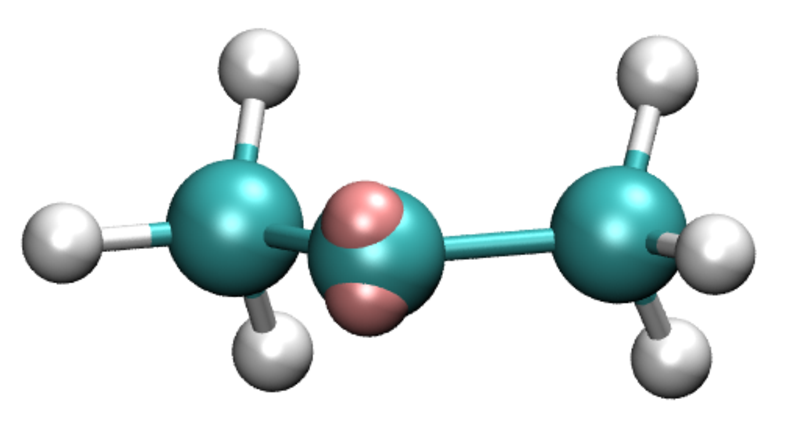
\includegraphics[width=3cm]{delta}}
& $\delta$ & $sp^3$ 2-electron \\
\hline
\end{tabular}
\end{center}
\end{table}

\subsection{The MOO program}

We wished to generalise the method developed in REF, so that it might be used for creating other pseudosystems. Building on the scripts we had developed above we created a general minimisation program, the Multiple Orbital Optimiser (MOO), which could minimise the error between all-electron and pseudosystems. This program is written in Python~\cite{python}, and works on the following procedure:

\begin{enumerate}
\item Accept a series of pseudosystem calculations as an input. 
\item Accept a range of observable molecular properties as input, as well as reference, all-electron values for these properties.\footnote{In addition to the above, the user can also weight the various criteria as desired, thus altering the priority of the optimisation criteria.}
\item Attempt to minimise these differences iteratively by 
\begin{enumerate}
\item altering the pseudopotential parameters 
\item running the calculation(s) in Turbomole~\cite{TURBOMOLE}
\item measuring the properties specified in step 2 
\item calculating the differences between reference and pseudosystems
\end{enumerate}
\end{enumerate}

The minimisation itself is carried out via a Sequential Quadratic Programming (SQP) algorithm implemented in SciPy~\cite{scipy}. This method was chosen for the flexibility of the boundary constraints implemented in SciPy.

\subsection{The Optimisation Criteria}

A number of optimisation criteria were proposed and used in extracting potentials. They include: 

\begin{enumerate}
\item Molecular orbital energies
\item TDDFT excitation energies
\item UV spectra fitting
\item Total energy differences - Being able to fit potentials to energy differences between individual calculations means being able to fit to such properties as ionisation energies, singlet-triplet potential energy surface gaps, or even alternate geometries.
\end{enumerate}

Next the choice must be made as to which properties of the pseudosystem may be altered in the minimisation. As seen in Section~\ref{sec:pseudoform}, the pseudopotential functions have both coefficients and exponents that can be modified. There is also the spatial arrangement of the pseudopotentials themselves. For the $\alpha$ and $\beta$ potentials described in Table~\ref{tab:pseudodiags}, there are the distances $d$ and $c$, which can be altered by the MOO program in the course of the minimisation. The other potential setups in the following sections have their own geometric properties which may be altered.

\begin{table}
\begin{center}
\caption[Boundary conditions for pseudopotential optimisation.]{Boundary conditions for pseudopotential optimisation. $d$ is the distance between a pseudocarbon and its $s$ potentials. $c$ is the distance above and below the $xy$ plane of $s$ potentials in $\alpha$ and $\beta$ potentials.}
\label{tab:optboundaries}
\begin{tabular}{|c|.|.|}
\hline
\multicolumn{1}{|c|}{\textbf{Parameter}} & 
\multicolumn{1}{|c|}{\textbf{Lower Bound}} & 
\multicolumn{1}{|c|}{\textbf{Upper Bound}} \\
\hline
coefficients & -50.0 & 50.0 \\
exponents & 0.001 & 50.0 \\
 $d$ ($a.u.$) & 0.5 & 1.0 \\
 $c$ ($a.u.$) ($\alpha$ and $\beta$) & 0.25 & 1.0 \\
\hline
\end{tabular}
\end{center}
\end{table}

The boundary conditions used for the selection of pseudopotential parameters are listed in Table~\ref{tab:optboundaries}. It was observed in optimisations that weaker and more diffuse potentials that gave the correct results for the chosen optimisation system always transferred better to other systems than stronger and more concentrated potentials. This led to the decision that, rather than taking guesses entirely at random for the values of the gaussian coefficients and exponents, the values should be chosen from a normal distribution with a mean of $\mu$=0 and with a standard deviation half of that of the upper bound (\emph{i.e.} a standard deviation of $\sigma$=25.0).

\subsection{Interpreting the Results}

\begin{table}[h]
\begin{center}
\caption[An example pseudopotential optimisation table.]{An example optimisation run on a hypothetical pseudosystem. Column `Pseudocarbon $l$' shows the angular momenta for which potential functions have been applied. The `Criteria' column lists what reference values have been supplied for the program to attempt to match, as well as any weighting applied in brackets (). Finally, the `Best $H_{total}/N$' gives a normalised total error for the best result found by the minimisation program.}\label{tab:exampleopt}
\begin{tabular}{| c | c | c | c |}
\hline
\textbf{Carbon $l$} & 
\textbf{Basis} & 
\textbf{Criteria} & 
\textbf{Best $H_{total}/N$}\\
\hline
$s,p$ & def-SV(P) & \multicolumn{1}{m{3cm}}{\centering HOMO; HOMO-1($\times$2); IE} & 0.001 \\
\hline
\end{tabular}
\end{center}
\end{table}

With the range of criteria and parameters possible for optimising pseudopotentials, it becomes easier to follow results if the details are condensed into a regular format, described in this section.

Table~\ref{tab:exampleopt} displays the results of an example optimisation in a format designed to be as readable as possible. `Pseudocarbon $l$' is the list of all the angular momenta for which potential functions are applied to the central pseudocarbon atom. In this example, there is an $s$ and a $p$ potential, each with its corresponding coefficient and exponent. Under the `Criteria' heading, we see the reference criteria against which the minimiser works. In this example, our criteria are `HOMO' (the HOMO orbital energy), `HOMO-1' (the energy of the orbital \textit{below} the HOMO, the `HOMO-1th' orbital) and `IE', the ionisation energy. We also see that the `HOMO-1' criteria has a $\times2$ weighting. Most of the various criteria on which the potentials are optimised can be written in terms of energy, which allows us to normalise the final error $H_{total}$ by dividing it by the number of criteria (multiplied by any individual weighting applied to them).

In the sections that follow, results generated using optimised pseudopotentials will be presented first. They will then be followed by the details of the optimisation.

- Spectral optimisation?

%\subsection*{\sffamily \large Geometry Optimisation}
%\label{section:geometry_optimisation}		    		  
%  Using pseudo-potential calculations for geometry optimisation presents some difficulties. Designing pseudo-potentials such that the explicitly-treated parts of the molecule experience the correct attraction and repulsion at a particular geometry is one thing, designing them such that the same is true at any (reasonable) geometry is quite another. With a little knowledge of the all-electron system however, we can ensure that the pseudo-system will fall into the correct geometry.	
% 		 
% We begin by finding curves of dissociation for the explicit and pseudo-potential parts of the molecule, as well as another for the same parts of the all-electron molecule (see Figure \ref{figure:dissociation_diagram}). We then use a nonlinear least-squares Marquardt-Levenburg algorithm to fit a simple, exponentially-decreasing function (of the form MNMN) to the difference between thsese two curves. We can now use this to make an energy correction to the pseudo-system. 		
%
%  		  
% We want the total energy of the system to be a minimum and the energy gradients on the explicitly-treated atoms to be zero at the true geometry (this needn't be true of the pseudo-atoms, see below). We have the correction for the total energy, and by taking the derivative of the fitted function, we have a measure of whether the explicit and pseudo-potential parts of the molecule experience an overall attraction or repulsion, as well as an estimate of its magnitude. We assume the effect of the potentials on the explicit hydrogen atoms is small, and add our gradient correction directly to the potential felt along the carbon-pseudo-carbon axis by one carbon, whilst subtracting it from the potential felt by the other. By doing this at every step of the optimisation, the carbon-pseudo-carbon distance should naturally reach the correct value.	
% 		 
% Finally, the pseudo-atoms are fixed relative to each other before starting the optimisation.		
% 		 
%\begin{figure}
%%\includegraphics[scale=8cm]{ethene_dissociation}	
%\begin{center}		 
%\end{center}		
%\vspace{0.25in}		 
%\hspace*{3in}		
%\caption{Diagram of dissociation curves for all-electron and pseudo-molecular calculations.}		
%\label{figure:dissociation_diagram}
%\end{figure}		

\section{Results and discussion} 

\subsection{$\beta$ potentials: $sp^{2}$ two-electron pseudofragment}

In order to have an explicit, all-electron system interact succesfully with an $sp^2$ pseudosystem, an $sp^2$ carbon potential that is capable of both $\pi$ and $\sigma$ bonding is required. The easiest way to create one is to add one more electron to the $\alpha$ potential setup, allowing it to bond to a nearest neighbour. This means that one of the $s$ potential sets can be removed, as these were intended to recapture the effect of $\sigma$ electrons which, in the $\alpha$ potential setup, are no longer there. The $sp^2$, two-electron pseudocarbon is depicted in Table~\ref{tab:pseudodiags}, as one half of an ethylene molecule.

Once optimised, these pseudopotentials were then transferred to a range of different molecules for testing, chosen to expose the pseudopotentials to a range of different chemical environments. The molecules, along with the sites of the pseudopotentials, are shown in Table~\ref{tab:beta_geoms}.

\begin{table}[h]
\begin{center}
\caption[$\beta$ test molecule set diagrams.]{Molecules used to test $\beta$ pseudopotentials. The pseudofragments are denoted by C$^\ast$.}
\label{tab:beta_geoms}
\begin{tabular}{|c|c|c|}
\hline
\thead{Name \\ Formula} & \thead{Pseudomolecular \\ Structure} \\
\hline 
\makecell{Ethene \\ C$_2$H$_4$} & 
\chemfig{
     C^\ast% 1
    =C% 2
}\\
\hline
\makecell{Formaldehyde \\ CH$_2$O} & \chemfig{
     C^\ast% 1
    =O% 2
}\\
\hline
\makecell{Ethenol \\ CH$_2$CHOH} & \begin{tabular}{c} \\\chemfig{
              C^\ast% 1
       =[:330]% 2
    -[:30,,,1]OH% 3
}\\ \\\end{tabular}\\
\hline
\makecell{Methanimine \\ CH$_2$NH} & \chemfig{
              C^\ast% 1
    =[,,,1]NH% 2
}\\
\hline
\makecell{Ethylamine \\ CH$_2$CHNH$_2$} & \begin{tabular}{c} \\\chemfig{
              C^\ast% 1
       =[:330]% 2
    -[:30,,,1]NH_2% 3
}\\ \\\end{tabular}\\
\hline
\end{tabular}
\end{center}
\end{table}

Figure~\ref{fig:beta_graphs} displays results for the HOMO energy, first ionisation energy, singlet-triplet gap energy and first excitation energy across the range of different test molecules using $\beta$ potentials. The majority of the results can be seen immediately to be of a similar quality to the first pseudopotentials of Sections~\ref{sec:prototype_work} and \ref{sec:alpha_results}, and well within half an electron-volt of the all-electron values. The pattern which emerges is that for systems where the potentials are bonded to carbon, the error is relativity small, but where the pseudocarbon bond is to another element such as oxygen (CH$_2$O), or nitrogen (CH$_2$NH), then the errors are larger, up to around 30\%. Given the potentials are optimised on a potential system bonded to a real carbon, this is probably to be expected. Bonds between carbon atoms have a very different character to bonds between carbon and oxygen or nitrogen atoms.

\begin{figure}
\caption[Energy level results for $\beta$ pseudopotentials.]{DFT and TDDFT-PBE0 comparison of all-electron and pseudosystem energies across a range of $\beta$ potential systems.}
\begin{center}
\includegraphics[width=8cm]{beta_pbe0}
\label{fig:beta_graphs}
\end{center}
\end{figure}

This trend is quantified in Table~\ref{tab:beta_errors}, where the mean difference between all-electron and pseudosystems across a range of properties is shown, broken down by the type of C$^\ast$-X bond at the pseudo/all-electron interface. When X is carbon, pseudosystem values for DFT-PBE0 calculations are consistently within 6\% of the all-electron system values, for all recorded properties. Where X is oxygen or nitrogen however, the DFT-PBE0 mean differences range from 14.7\% to 63.7\%.

\begin{table}
\begin{center}
\caption[Error results for $\beta$ pseudopotentials.]{Average errors for molecules using $\beta$ potentials, arranged by pseudocarbon-X bond type, for HF, DFT-PBE0, TD-HF and TDDFT calculations.}\label{tab:beta_errors}
\begin{tabular}{| c |.|.|.|.|}
\hline
\multicolumn{1}{|c|}{\textbf{Bond Type}} & 
\multicolumn{4}{|c|}{\textbf{Mean Error ($\%$)}} \\
\multicolumn{1}{|c|}{\textbf{(C$^\ast$-X)}} & \multicolumn{1}{|c|}{\textbf{$\Delta_{S-T}$}} &
\multicolumn{1}{|c|}{\textbf{HOMO}} & 
\multicolumn{1}{|c|}{\textbf{1$^{st}$ I.E.}} & 
\multicolumn{1}{|c|}{\textbf{1$^{st}$ Ex}} \\
\hline
\multicolumn{5}{|c|}{Hartree-Fock} \\
\hline
All & 92.4 & 8.6 & 29.7 & 9.3 \\
C$^\ast$-C & 19.1 & 1.9 & 12.4 & 4.1 \\
C$^\ast$-O & 397.6 & 28.6 & 90.0 & 24.0 \\
C$^\ast$-N & 7.4 & 8.8 & 21.1 & 10.0 \\
\hline
\multicolumn{5}{|c|}{DFT-PBE0} \\
\hline
All & 18.4
& 18.1
& 15.2
& 17.5
\\
C$^\ast$-C & 5.5
& 5.9
& 5.5
& 2.0
\\
C$^\ast$-O & 60.6
& 43.3
& 35.6
& 63.7
\\
C$^\ast$-N & 14.7
& 29.4
& 24.1
& 18.1
\\
\hline
\end{tabular}
\end{center}
\end{table}

\begin{table}
\begin{center}
\caption{Optimisation criteria and parameters for the best $\beta$ potential set.}
\label{tab:beta_opt_results}
\begin{tabular}{| c |.| c | c | c |}
\hline
\textbf{Carbon $l$} & 
\multicolumn{1}{|c|}{\textbf{Basis}} & 
\multicolumn{2}{|c|}{\textbf{Criteria}} & \textbf{$H_{total}/N$ ($eV$)} \\
\hline
$p$ & \multicolumn{1}{|c|}{def-SV(P)} & \multicolumn{2}{|m{2cm}|}{\centering HOMO(*3); HOMO-1; HOMO-2} & 0.90670 \\
\hline
\textbf{potential} & 
\multicolumn{1}{|c|}{\textbf{Coefficient}} 
& \multicolumn{1}{|c|}{\textbf{Exponent}} & \textbf{$d$ ($a.u.$)} & \textbf{$c$ ($a.u.$)} \\
\hline
p & -2.0031 & 0.4694 & - & - \\
s & 0.4376 & 0.4946 & 0.5 & 0.25 \\
\hline
\end{tabular}
\end{center}
\end{table}

Contained in Table~\ref{tab:beta_opt_results} are the details of the $\beta$ optimisation. The optimisation used as its reference the top three occupied orbitals in a closed-shell Hartree-Fock calculation on ethylene, with a 3$\times$ weighting on the HOMO orbital, and the normalised total error is 0.9067~$eV$. Overall, this pseudopotential setup does not differ greatly from the $\alpha$ pseudopotentials, other than that these potentials are slightly weaker and more diffuse than the $\alpha$ potentials. 

\subsection{$\gamma$ potentials: $sp^{3}$ one-electron pseudofragment}

It was decided to create a one-electron pseudopotential for an $sp^3$ pseudocarbon, and to  optimise it to mimic a methyl group bonded to a carbon atom. This setup has a $p$-shaped potential on the central carbon, along with three $s$-shaped potentials replacing the hydrogen atoms at a distance from the central carbon of 0.5~$a.u.$. The setup is shown in Table~\ref{tab:potential_definitions}.

Once optimised, the pseudopotentials were again transferred to a set of test molecules, shown in Table~\ref{tab:gamma_geoms} along with the sites of the pseudopotentials.

\begin{table}
\begin{center}
\caption[$\gamma$ test molecule set diagrams.]{Molecules used to test $\gamma$ pseudopotentials. The pseudofragments are denoted by C$^\ast$.}
\label{tab:gamma_geoms}
\begin{tabular}{|c|c|}
\hline
\thead{Name \\ Formula} & \thead{Pseudomolecular \\ Structure} \\
\hline
\makecell{Ethane (eclipsed) \\ CH$_3$CH$_3$} & \chemfig{
     C^\ast% 1
    -CH_3% 2
}\\
\hline
\makecell{Methanol \\ CH$_3$OH} & \chemfig{
              C^\ast% 1
    -[,,,1]OH% 3
}\\
\hline
\makecell{Methylamine \\ CH$_3$NH$_2$} & \chemfig{
              C^\ast% 1
    -[,,,1]NH_2% 2
}\\
\hline
\makecell{Ethanoic Acid \\ CH$_3$COOH} & \begin{tabular}{c} \\\chemfig{
           C^\ast% 1
     -[:90]% 2
              (
     -[:30,,,1]OH% 4
              )
    =[:150]O% 3
}\\ \\\end{tabular}\\
\hline
\makecell{Aspirin \\ C$_9$H$_8$O$_4$} & \begin{tabular}{c} \\\chemfig{
            C^\ast% 1
      -[:60]% 2
               (
         =[:120]O% 3
               )
           -O% 4
     -[:300]% 5
    =^[:240]% 6
     -[:300]% 7
          =^% 8
      -[:60]% 9
    =^[:120]% 10
               (
         -[:180]% -> 5
               )
      -[:60]% 11
               (
         -[,,,1]OH% 13
               )
     =[:120]O% 12
}\\ \\\end{tabular}\\
\hline
\makecell{Methane \\ CH$_4$} & \chemfig{
    C^\ast -H% 1
}\\
\hline
\makecell{Ethanal \\ C$_2$H$_4$O} & \begin{tabular}{c} \\\chemfig{
           C^\ast% 1
    -[:330]% 2
     =[:30]O% 3
}\\ \\\end{tabular}\\
\hline
\makecell{Adapted from \\ Reference~\cite{nava2012bonding} \\ ClAuP(CH$_3$)$_3$} & \begin{tabular}{c} \\\chemfig{
           C^\ast% 2
    -[:310]P% 1
              (
        <[:230]C^\ast% 3
              )
              (
       <:[:180]C^\ast% 4
              )
          -Au% 5
          -Cl% 6
} \\ \\\end{tabular}\\
\hline
\end{tabular}
\end{center}
\end{table}

In Figure~\ref{fig:gamma_graphs} we see results for the HOMO, first ionisation, singlet-triplet gap and first TDDFT excitation energies for the different molecular systems incorporating a $\gamma$ potential. These molecules included pseudofragments bonded to groups including -OH, -NH$_2$, -COOH and an aromatic ring. Figure~\ref{fig:gamma_graphs} shows us that the results are mostly close to the reference system values. There are however, notable differences in the ionisation and singlet-triplet gap energies of methanol in the pseudosystem with respect to the all-electron system. In this case the $\gamma$ pseudocarbon is bonded to an oxygen atom. In the $\beta$ potential system described above, a pseudocarbon being bonded to a non-carbon atom resulted in significant differences between all-electron and pseudosystems. Whilst in Figure~\ref{fig:gamma_graphs} this remains true for the singlet-triplet gap and ionisation energy of the one pseudocarbon-oxygen bond in our test set, the HOMO and first-excitation energies appear to be sound. One notes also that the C$^\ast$-N bond of CH$_3$NH$_2$ does not appear to have caused any problems for this pseudopotential, with all the pseudo/reference mean differences being comparable in all cases to those of the C$^\ast$-C systems. 

\begin{figure}
\begin{center}
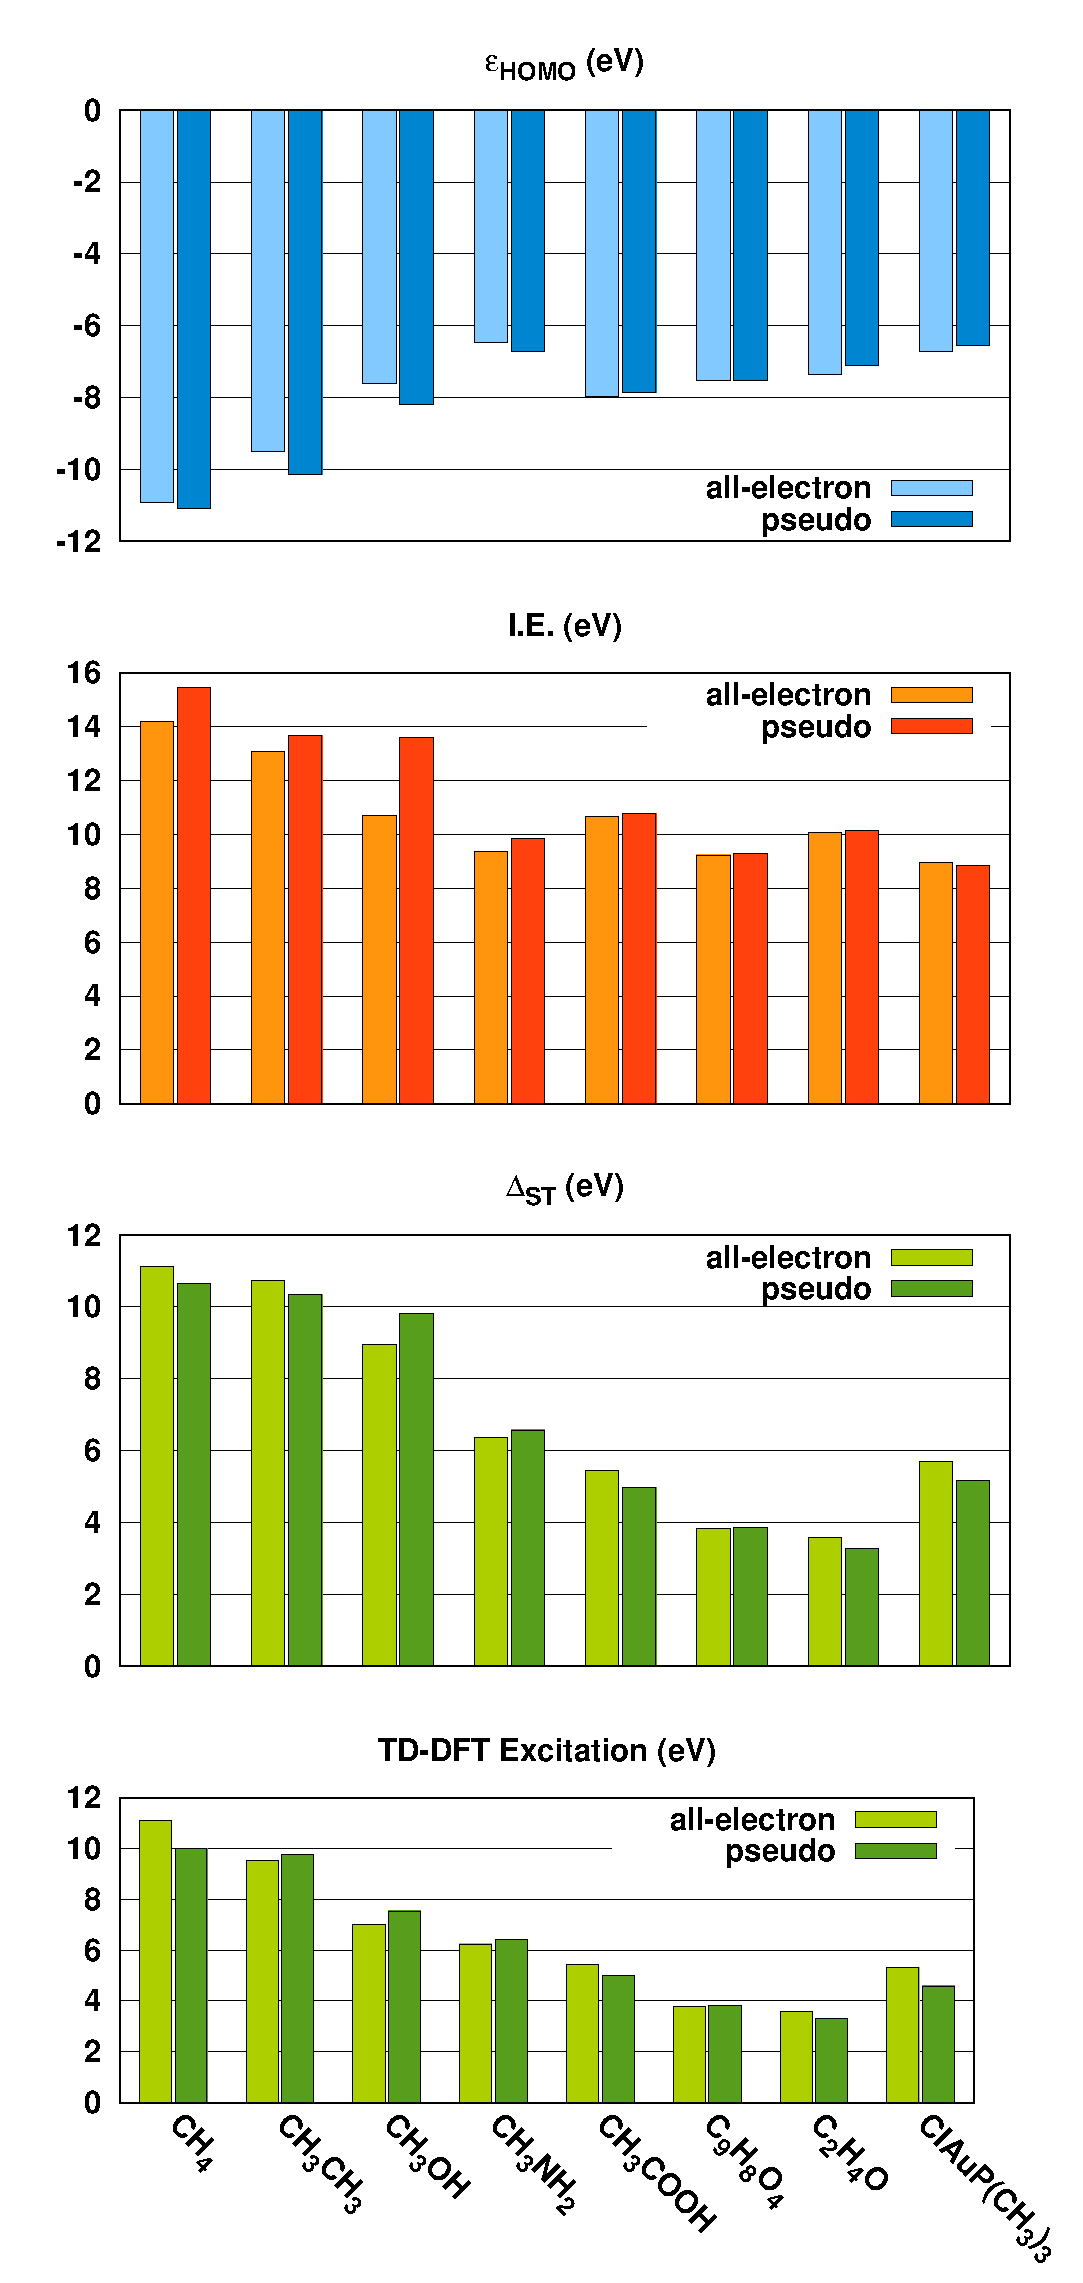
\includegraphics[width=8cm]{gamma_pbe0}
\end{center}
\caption[Energy level results for $\gamma$ pseudopotentials.]{DFT and TDDFT-PBE0 comparison of all-electron and pseudosystem energies across a range of $\gamma$ potential systems.}\label{fig:gamma_graphs}
\end{figure}

Table~\ref{tab:gamma_errors} breaks down the results above more clearly, showing the reader the mean difference between all-electron and pseudosystems across a range of properties (HOMO, 1$^{st}$ ionisation, singlet-triplet gap and 1$^{st}$ TDDFT excitation energies), broken down by the type of C$^\ast$-X bond at the pseudo/all-electron interface. The worst results are to be seen where X is either oxygen or phosphorus, with mean differences from the all-electron systems ranging up to 13.7\% (the 1$^{st}$ excitation energy of the ClAuPC(CH$_3$)$_3$ molecule). In the particular case of the C$^\ast$-P results, it is worth noting that the pseudosystem is built with three separate sets of $\gamma$ potentials, which would likely have compounded any error in the potentials themselves. The C$^\ast$-H bond of methane has also caused difficulties, with ionisation and excitation energies significantly above those of C$^\ast$-C systems. The fact however that the C$^\ast$-N bond gives mean differences similar to those of C$^\ast$-C systems, combined with the fact that the overall differences between all-electron and pseudosystems for non-carbon-bonded pseudocarbons are much lower than those of the $\beta$ potentials, suggests that either the $\gamma$ potentials we have optimised are more transferable than the $\beta$ potentials, or that methyl groups are simply easier to reproduce than $sp^2$ -CH$_2$ groups.

\begin{table}
\caption[Error results for $\gamma$ pseudopotentials.]{Average errors for molecules using $\gamma$ potentials, arranged by pseudocarbon-X bond type, for both HF and DFT-PBE0 calculations.}
\label{tab:gamma_errors}
\begin{center}
\begin{tabular}{| c |.|.|.|.|}
\hline
\textbf{Bond Type} & 
\multicolumn{4}{|c|}{\textbf{Mean Difference ($\%$)}} \\
\multicolumn{1}{|c|}{\textbf{(C$^\ast$-X)}} & 
\multicolumn{1}{|c|}{\textbf{$\Delta_{S-T}$}} & 
\multicolumn{1}{|c|}{\textbf{HOMO}} & 
\multicolumn{1}{|c|}{\textbf{1$^{st}$ I.E.}} & 
\multicolumn{1}{|c|}{\textbf{1$^{st}$ Ex}} \\
\hline
\multicolumn{5}{|c|}{Hartree-Fock} \\
\hline
All
& 12.2
& 2.9
& 6.6
& 4.1
\\
C$^\ast$-C
& 6.6
& 2.4
& 1.6
& 5.8
\\
C$^\ast$-O
& 27.5
& 6.2
& 26.0
& 1.9
\\
C$^\ast$-N
& 19.0
& 1.6
& 2.7
& 6.1
\\
C$^\ast$-H
& 5.4
& 1.2
& 6.9
& 5.7
\\
C$^\ast$-P
& 4.0
& 2.8
& 11.9
& 0.2
\\
\hline
\multicolumn{5}{|c|}{DFT-PBE0} \\
\hline
All 
& 5.1
& 3.9
& 7.7
& 4.3
\\
C$^\ast$-C 
& 5.3
& 2.8
& 1.7
& 4.6
\\
C$^\ast$-O 
& 9.5
& 7.8
& 12.4
& 7.7
\\
C$^\ast$-N
& 3.1
& 3.8
& 4.9
& 2.9
\\
C$^\ast$-H
& 4.3
& 1.5
& 8.8
& 9.8
\\
C$^\ast$-P
& 9.0
& 2.3
& 1.3
& 13.7
\\
\hline
\end{tabular}
\end{center}
\end{table}

\begin{table}[h]
\begin{center}
\caption{Optimisation criteria and parameters for the best $\gamma$ potential set.}\label{tab:gamma_opt_results}
\begin{tabular}{|c|.|.|c|c|}
\hline
\textbf{Carbon $l$} & 
\multicolumn{1}{|c|}{\textbf{Basis}} & \multicolumn{2}{|c|}{\textbf{Criteria}} & \textbf{$H_{total}/N$ ($eV$)} \\
\hline
$s,p$ & \multicolumn{1}{c}{def-SV(P)} & \multicolumn{2}{|m{2.5cm}|}{HOMO($\times$2); HOMO-1} & 0.4179 \\
\hline
\textbf{Potential} & 
\multicolumn{1}{|c|}{\textbf{Coefficient}} & 
\multicolumn{1}{|c|}{\textbf{Exponent}} & \textbf{$d$ ($a.u.$)} & \textbf{$c$ ($a.u.$)} \\
\hline
$p$ & -2.0949 & 0.3951 & - & - \\
$s$ & 38.5052 & 14.8328 & 0.5 & - \\
\hline
\end{tabular}
\end{center}
\end{table}

Contained in Table~\ref{tab:gamma_opt_results} are the details of the $\gamma$ optimisation. This optimisation was carried out on an eclipsed ethane molecule, using $s$ and $p$ central potentials, with the top two occupied orbitals as a reference (with the HOMO doubly-weighted). These $s$ potentials are far more concentrated than those of either of the $sp^2$ potentials. 

\subsection{$\delta$ potentials: $sp^{3}$ two-electron pseudofragment}

The final pseudopotentials designed were another $sp^3$ pseudocarbon configuration. In this pseudopotential setup, there are two electrons, so it is able to act as a bridge between two other all-electron, bonding atoms. This time the central carbon has not only a $p$-shaped potential, but also its own $s$-shaped potential, and we have $s$ potentials replacing two of the all-electron bonds at a distance from the pseudocarbon of $d$=0.5~$a.u.$. The setup is shown in Table~\ref{tab:potential_definitions} as part of a propane molecule, on which it is optimised.

\begin{table}
\begin{center}
\caption[$\delta$ test molecule set diagrams.]{Molecules used to test $\delta$ pseudopotentials. The pseudofragments are denoted by C$^\ast$.}
\label{tab:delta_geoms}
\begin{tabular}{|c|c|}
\hline
\thead{Name \\ Formula} & \thead{Pseudomolecular \\ Structure} \\
\hline
\makecell{Methane \\ CH$_4$} &
\begin{tabular}{c} \\\chemfig{
           H% 1
    -[:330]C^\ast% 2
     -[:30]H% 3
}
\\ \\\end{tabular}\\
\hline
\makecell{Fluoroacetic Acid \\ CH$_{2}$FCOOH}
&
\begin{tabular}{c} \\\chemfig{
           O% 3
     =[:30]% 2
              (
     -[:90,,,1]OH% 4
              )
    -[:330]C^\ast% 1
     -[:30]F% 5
}
\\ \\\end{tabular}\\
\hline
\makecell{Propane \\ CH$_{3}$CH$_{2}$CH$_{3}$}
& 
\begin{tabular}{c} \\\chemfig{
           CH_3% 1
    -[:330]C^\ast% 2
     -[:30]CH_3% 3
}
\\ \\\end{tabular}\\
\hline
\makecell{Ethanol \\ C$_{2}$H$_{5}$OH}
& 
\begin{tabular}{c} \\\chemfig{
              CH_3% 1
       -[:330]C^\ast% 2
    -[:30,,,1]OH% 3
}
\\ \\\end{tabular}\\
\hline
\makecell{Ethylamine \\ C$_{2}$H$_{5}$NH$_{2}$}
& 
\begin{tabular}{c} \\\chemfig{
              CH_3% 1
       -[:330]C^\ast% 2
    -[:30,,,1]NH_2% 3
}
\\ \\\end{tabular}\\
\hline
\makecell{Malonaldehyde \\ CHOCH$_{2}$CHO} & 
\begin{tabular}{c} \\\chemfig{
           O% 3
     =[:30]% 2
    -[:330]C^\ast% 1
     -[:30]% 4
    =[:330]O% 5
}
\\ \\\end{tabular}\\
\hline
\makecell{- \\ CHONH$_{2}$CH$_{2}$CHO} & 
\begin{tabular}{c} \\\chemfig{
           O% 3
     =[:30]% 2
    -[:330]C^\ast% 1
     -[:30]NH% 4
     -[:330]% 5
    =[:30]O% 6
}
\\ \\\end{tabular}\\
\hline
\end{tabular}
\end{center}
\end{table}

As above, these pseudopotentials were tested in a variety of small molecules, shown in Table~\ref{tab:delta_geoms} along with the sites of the pseudopotentials.

Displayed in Figure~\ref{fig:delta_graphs} are HOMO, 1$^{st}$ ionisation, singlet-triplet gap and 1$^{st}$ TDDFT excitation energies for the test molecules and pseudomolecules using $\delta$ potentials. Among them are pseudopotentials bonded to groups including -OH, -NH$_2$ and -COOH. For the great majority of these results the all-electron values are matched closely by the pseudosystems. Notable differences between all-electron and pseudosystem results are found however in methane, and in the 1$^{st}$ excitation energy of ethanol. This remains in keeping with the pattern seen in the other potential sets. In methane, the pseudoatom is bonded to two explicit hydrogen atoms. In ethanol, the pseudoatom is bonded to one explicit carbon atom and one explicit oxygen atom. This pseudopotential setup was optimised on propane, and so both methane and ethanol require the pseudofragment to form bonds for which it was not optimised.

\begin{figure}
\begin{center}
\includegraphics[width=8cm]{delta_pbe0}
\end{center}
\caption[Energy level results for $\delta$ pseudopotentials.]{DFT and TDDFT (PBE0) comparison of all-electron and pseudosystem energies across a range of $\delta$ potential systems.}\label{fig:delta_graphs}
\end{figure}

Further details are shown in Table~\ref{tab:delta_errors}, where the results are broken down according to the R-C$^\ast$-X bond type present between the pseudocarbon and its neighbours. The worst results are those of methane (H-C$^\ast$-H) with a 23.6\% difference in singlet-triplet gap energy and a 34.5\% difference in 1$^{st}$ excitation energy between pseudosystem and all-electron system for Hartree-Fock calculations, which does not reduce by much with DFT added. One reason for the particularly poor performance of methane is likely the fact that it is the only system for which both of the bonds of the pseudocarbon are formed with hetero-atoms. The C-C$^\ast$-N bonds, (those of ethylamine and CHONH$_2$CH$_2$CHO) give a poor singlet-triplet result under HF, but a good one under DFT-PBE0. This high average HF singlet-triplet gap error for molecules containing C-C$^\ast$-N bonds comes overwhelmingly from the CHONH$_2$CH$_2$CHO molecule (a 48\% difference in singlet-triplet gap energy as compared to the 7.1\% of ethylamine), and the reason for this may well be that in CHONH$_2$CH$_2$CHO both pseudocarbon bonds, while formed with explicit carbon atoms, are formed with $sp^2$ carbons, as opposed to the $sp^3$ carbons we see in propane (see Table~\ref{tab:pseudodiags}). Finally we note that under HF the propane pseudosystem itself has a 17.7\% singlet-triplet gap energy difference with its all-electron counterpart, but returns to a 5.3\% difference under DFT-PBE0. The reason for this is explored below.

\begin{table}[h]
\begin{center}
\caption[Error results for $\delta$ pseudopotentials.]{Average errors for molecules using $\delta$ potentials, arranged by pseudocarbon-X bond type, for both HF and DFT-PBE0 calculations.}\label{tab:delta_errors}
\begin{tabular}{| c |.|.|.|.|}
\hline
\textbf{Bond Type} & 
\multicolumn{4}{|c|}
{\textbf{Mean Difference ($\%$)}} \\
\multicolumn{1}{|c|}{\textbf{(R-C$^\ast$-X)}} & 
\multicolumn{1}{|c|}{\textbf{$\Delta_{S-T}$}} & 
\multicolumn{1}{|c|}{\textbf{HOMO}} & \multicolumn{1}{|c|}{\textbf{1$^{st}$ I.E.}} & 
\multicolumn{1}{|c|}{\textbf{1$^{st}$ Ex}} \\
\hline
\multicolumn{5}{|c|}{Hartree-Fock} \\
\hline
All
& 18.1
& 1.6
& 5.0
& 11.5
\\
H-C$^\ast$-H
& 23.6
& 5.3
& 9.6
& 34.5
\\
C-C$^\ast$-C
& 17.7
& 0.2
& 4.1
& 8.9
\\
C-C$^\ast$-O
& 9.4
& 0.8
& 4.2
& 13.3
\\
C-C$^\ast$-N
& 27.6
& 0.9
& 4.5
& 6.2
\\
C-C$^\ast$-F
& 3.0
& 2.9
& 3.8
& 2.7
\\
\hline
\multicolumn{5}{|c|}{DFT-PBE0} \\
\hline
All
& 8.9
& 3.1
& 2.3
& 10.5
\\
H-C$^\ast$-H
& 25.0
& 9.3
& 6.9
& 26.8
\\
C-C$^\ast$-C
& 5.3
& 0.2
& 0.9
& 2.8
\\
C-C$^\ast$-O
& 12.7
& 2.9
& 0.3
& 25.7
\\
C-C$^\ast$-N
& 5.5
& 2.5
& 1.1
& 5.9
\\
C-C$^\ast$-F
& 2.8
& 4.2
& 4.8
& 3.4
\\
\hline
\end{tabular}
\end{center}
\end{table}

\begin{table}[h]
\begin{center}
\caption{Optimisation criteria and parameters for the best $\delta$ potential set.}\label{tab:delta_opt_results}
\begin{tabular}{| c |.|.|.|c|}
\hline
\textbf{Carbon $l$} & 
\multicolumn{1}{|c|}{\textbf{Basis}} & 
\multicolumn{2}{|c|}{\textbf{Criteria}} & \multicolumn{1}{|c|}{\textbf{$H_{total}/N$ ($eV$)}} \\
\hline
\multicolumn{1}{|c|}{$s, p$} &
\multicolumn{1}{|c|}{def-SV(P)} & \multicolumn{2}{|m{2cm}|}{\centering \makecell{HOMO;\\ HOMO-1;\\ HOMO-2;\\ HOMO-3;\\ HOMO-4;\\ HOMO-5}} & 0.40067 \\
\hline
\multicolumn{1}{|c|}{\textbf{Potential}} & 
\multicolumn{1}{|c|}{\textbf{Coefficient}} & 
\multicolumn{1}{|c|}{\textbf{Exponent}} & 
\multicolumn{1}{|c|}{\textbf{$d$ ($a.u.$)}} & 
\multicolumn{1}{|c|}{\textbf{$c$ ($a.u.$)}} \\
\hline
\multicolumn{1}{|c|}{$p$} & 
-6.9569 & 3.4066 & \multicolumn{1}{|c|}{-} & - \\
\multicolumn{1}{|c|}{$s$} & 
5.3934 & 6.4912 & 0.5 & - \\
\multicolumn{1}{|c|}{$s$ (carbon)} & 
0.6391 & 0.9382 & \multicolumn{1}{|c|}{-} & - \\
\hline
\end{tabular}
\end{center}
\end{table}

Table~\ref{tab:delta_opt_results} details the optimisation criteria and parameters for the $\delta$ potential setup. These are optimised on propane and use both a $p$ potential and an $s$ potential on the central pseudocarbon, in addition to the non-atom-centred $s$ potentials. The reference criteria used are the six highest-occupied molecular orbitals of an Unrestricted Hartree-Fock calculation.

Optimisation on this molecule is complicated by the fact that the highest occupied molecular orbtials are all within around 1~$eV$ of one another, making it very easy for the orbitals to end up in the wrong order if care is not taken. This is the reason for the significant change in accuracy between the propane singlet-triplet gap under HF and under DFT-PBE0 in Table~\ref{tab:delta_errors}. 

\section{Absorption spectra of Pseudomolecules}
\label{sec:spectraloptimisation}

It was shown in REF that $\alpha$ pseudopotentials could accurately reproduce absorption spectra for the excitations of the remaining electrons in the systems (obviously as the pseudopotential calculations contain only $\pi$ orbitals, excitations to or from $\sigma$ orbitals cannot be reproduced). It was shown that all the peaks of the reference spectra were clearly identifiable in the pseudosystem spectra, and these peaks in the pseudosystem spectra have very similar intensities and relative frequencies to their all-electron counterparts. We did however see that the pseudosystem spectra were consistently shifted by a 30-40~$nm$ as compared to the all-electron spectra.

\begin{figure}
\begin{center}
\includegraphics[width=8.5cm]{rings_geom1_rpas}
\end{center}
\caption[PAH and pseudo-PAH UV spectra: $geom_1$]{Comparison of the absorption spectra for the 20 first singlet excitations obtained with
$geom_1$ pseudopotentials (ps) and all-electron (ref) calculations (def2-SV(P)(s-less)/TD-PBE0) within the RPA
framework.}\label{fig:rings_geom1_rpas}
\end{figure}

Figure~\ref{fig:rings_geom1_rpas} displays the same excitations for the same series of ring systems as Figure~\ref{fig:rings_set4_rpa}, however this time the pseudopotentials are a new set, $geom_1$. This set of pseudopotentials is optimised specifically with the reproduction of UV spectra in mind, and the details of this optimisation are described below in Section~\ref{sec:spectralopt}.

The improvement we desired for these spectra was to shift them closer to the all-electron spectra, and from Figure~\ref{fig:rings_geom1_rpas} we can see this has been achieved. Most of the peaks of the pseudosystem spectra overlap exactly with their all-electron counterparts, though it does seem there has been a very slight visible decrease in the overall intensity of the pseudosystem spectra, for example in the highest-energy peak in the pyrene spectrum.

Unfortunately, the $geom_1$ pseudopotentials were unable to produce spectra for triplet excitations in the manner of the $set4$ potentials, as the $\pi^{*}$ triplet state was lower in energy than the singlet state. This is discussed further below.

Overall this is a very pleasing result, given not only the degree of overall simplification of the pseudosystems compared to the all-electron systems, but also given the fact that the only `training set' used to optimise these potentials was a lone ethylene molecule treated only at the Hartree-Fock level. This pseudopotential method can be said to accurately reproduce UV absorption spectra.

\paragraph{Intruder Orbitals:} In Section~\ref{sec:mcpmethod} it was noted that the MCP method had the problem of the so-called `intruder orbitals'. These are the dormant orbitals which have been projected into the virtual space by the potentials. In Section~\ref{sec:alpha_results} only the first exitation was calculated, and the intruder orbitals were not to be seen. At higher-energy excitations however, there is a risk that the pseudosystems will produce extra peaks not present in the all-electron system. Ultimately we did not see any such peaks for the PAHs. Nevertheless, this is discussed as a possible area for improvement of the method in Section~\ref{sec:further_development}.

\subsection{Optimisation for Spectra}
\label{sec:spectralopt}

The measure of success for potentials so far, both in this work and the previous work REF, has been their ability to reproduce the HOMO, 1$^{st}$ ionisation and 1$^{st}$ excitation energies of the all-electron systems they replace. Following the success of the previous work in reproducing the spectra of PAHs, an effort was made to optimise pseudopotentials specifically for the reproduction of UV spectra. It was decided that three approaches should be tested for the creation of such potentials:

\begin{enumerate}
\item Using the virtual orbitals as reference criteria
\item Using TDDFT excitation energies as reference criteria
\item Fitting the spectra directly via a least-squares method
\end{enumerate}

Using these criteria we generated a great many potentials, most of which were poor fits, either to the reference system on which they were optimised or when transferred to other systems. Various problems were encountered with the use of TDDFT energies and with direct spectra fitting.

Ultimately, using the virtual orbitals as reference criteria was found to be the most successful of the techniques tested. Table~\ref{tab:geom1opt_results} summarises the optimisation of the $geom_1$ potential seen in the UV spectra comparison above. One notes looking at the results that the pseudopotential parameters found by the optimiser are not dissimilar to those of the original $set4$ potentials. The coefficients and exponents are all within 0.5 of those of $set4$, and incorporating the distances $d$ and $c$ (see Section~\ref{sec:prototype_work}) into the optimisation procedure has resulted in the non-atom-centered $s$ potentials being moved by less than 0.1~$a.u.$ in both directions.

\begin{table}[h]
\begin{center}
\caption[Optimisation of $geom_1$ pseudopotentials.]{List of optimisation criteria and results for the $geom_1$ pseudopotential set. This is an $\alpha$ potential using ethylene as a reference.}\label{tab:geom1opt_results}
\begin{tabular}{|c|.|.|c|c|}
\hline 
\textbf{Carbon $l$} & 
\multicolumn{1}{|c|}{\textbf{Basis}} &
\multicolumn{2}{|c|}{\textbf{Criteria}} & \textbf{$H_{total}/N$ ($eV$)} \\
\hline
$p$ & 
\multicolumn{1}{|c|}{def-SV(P)} & 
\multicolumn{2}{|m{2cm}|}{\makecell{HOMO;\\ HOMO+1;\\ HOMO+2}} & 0.04037 \\
\hline
\textbf{Potential} & 
\multicolumn{1}{|c|}{\textbf{Coefficient}} & 
\multicolumn{1}{|c|}{\textbf{Exponent}} & 
\textbf{$d$ ($a.u.$)} & \textbf{$c$ ($a.u.$)} \\
\hline
$p$ & -3.9020 & 0.6914 & - & - \\
$s$ & 1.2266 & 0.5448 & 0.5821 & 0.2689 \\
\hline
\end{tabular}
\end{center}
\end{table}

The significant difference between the potentials of the previous work and the $geom_1$ potentials of Table~\ref{tab:geom1opt_results} is in the optimisation criteria chosen. Rather than the HOMO, 1$^{st}$ ionisation and singlet-triplet gap energies chosen for $set_4$, the $geom_1$ potentials are optimised on the HOMO energy, as well as the first two virtual orbitals. This includes the $\pi^*$ orbital. The success of this potential as shown above means that ensuring these virtual orbitals are correct is crucial for the accurate reproduction of the spectrum, as one would expect. 

All all-trans-polyene and PAH molecules shown in Section~\ref{sec:alpha_results} were then retested using the $geom_1$ pseudopotentials. As noted above in Section~\ref{sec:spectraloptimisation}, the $geom_1$ pseudopotentials were not able to reproduce triplet excitations, and so the results were obtained only for the 1$^{st}$ ionisation energy and the HOMO energy of each molecule. The average percentage difference between all-electron and pseudosystems for the 1$^{st}$ ionisation and HOMO energies respectively were 0.8\% and 15.2\%. It is apparent from these results that while the use of virtual orbitals improved the ability of the $geom_1$ potentials to reproduce the spectra of the PAH molecules, their ability to reproduce the HOMO energy for the same test molecules was decreased, with errors significantly larger compared to the $set4$ percentage errors of Section~\ref{sec:alpha_results}. This will be a consequence of changing the reference criteria. The 1$^{st}$ ionisation energy of ethylene used in the $set4$ optimisation will still depend heavily on the $\pi$ orbital of ethylene even if it is only half-occupied. The same is true of the singlet-triplet gap energy. This may not be so true of the excitation energies. The fact that the $geom_1$ potentials do not use any part of the ethylene triplet energy surface in their optimisation criteria, unlike the $set4$ potentials, also seems a likely explanation for the fact that the $geom_1$ potentials are unable to reproduce the triplet excitation spectra above.

Overall then, it can be said that the use of virtual orbitals as reference criteria for optimisation improves the UV spectra produced. Simultaneously however, losing the singlet-triplet gap and 1$^{st}$ ionisation energies as reference criteria has an adverse effect on the ability of pseudopotential systems to reproduce these characteristics. 

The above suggests that tuning pseudopotentials to reproduce certain physical characteristics of molecules is possible, but that it is easy to bias potentials with the choice of reference criteria. Finding all-electron reference criteria that will allow the optimisation of general, `all-purpose' pseudopotentials is therefore difficult. 

In the rest of this work we are primarily interested in molecular spectra and so use the $geom_1$ pseudopotentials as a preference, though we also use and make comparisons with the original $set4$ potentials.

\paragraph{Removal of basis functions:} We found that it was possible to remove the $s$ basis functions of the def-SV(P) $geom_1$ pseudocarbon without altering any of the $geom_1$ results. This is promising, as fewer basis functions means a greater gain in computational efficiency. Henceforth in this work, the $geom_1$ potentials are used without $s$ functions.

\section{Pseudopotential Studies of Complex Systems}

Thus far, all potentials have been tested on systems related closely to those for which they have been optimised. In this section, the various potentials are tested in a series of more complex systems involving heavy atoms, distorted $\pi$ systems, and neighbouring $\pi$ rings. These systems were selected from recent literature with the aim of testing the limits of the potential methods thus-far described with their complex molecular and electronic structures. They are focused most heavily on the $\alpha$-type potentials. All four pseudosystems detailed in Section~\ref{sec:simple_systems} make an appearance, however.

\subsection{Complex Spectra: Helicene}
\label{sec:helicene}

In the previous work REF we studied the absorption and ECD spectra of helicene. We now repeat the same calculations on a series of [n]helicene molcules (of length $n$=6-9 rings) using the $geom_1$ potentials.

\begin{figure}
\begin{center}
\includegraphics[width=8cm]{pbe0_grand_rpas_geom1.png}
\end{center}
\caption[Computed all-electron and pseudopotential spectra for helicenes: $geom_1$]{Helicene UV and ECD spectra, for all-electron (red) and $geom_1$ pseudopotential (blue) systems. Calculations are performed at the TDDFT-PBE0 level.}\label{fig:helispectrageom1}
\end{figure}

Figure~\ref{fig:helispectrageom1} displays UV and ECD spectra for a range of helicene systems, with spectra for both all-electron and pseudomolecules, using the $geom_1$ pseudopotentials from Section~\ref{sec:spectraloptimisation}. Comparing the spectra for $geom_1$ and $set4$ potentials, the first thing to note in is that the $geom_1$ potentials do not require a shift in wavelength in order to line up the pseudosystem spectra with the all-electron spectra, which is an improvement. Other differences between the two pseudopotentials are present, but are more subtle. $set4$ appears to generate more low-energy peaks that are not present in the reference spectra (particularly for the ECD spectra), whereas $geom_1$ has additional peaks at the high-energy end of the spectra. As noted in Section~\ref{sec:spectraloptimisation}, the high-energy peaks are not necessarily unphysical. Aside from this the two pseudopotential spectra are very similar, both in the distribution of peaks and in their intensity.

\begin{figure}
\begin{tabular}{cc}
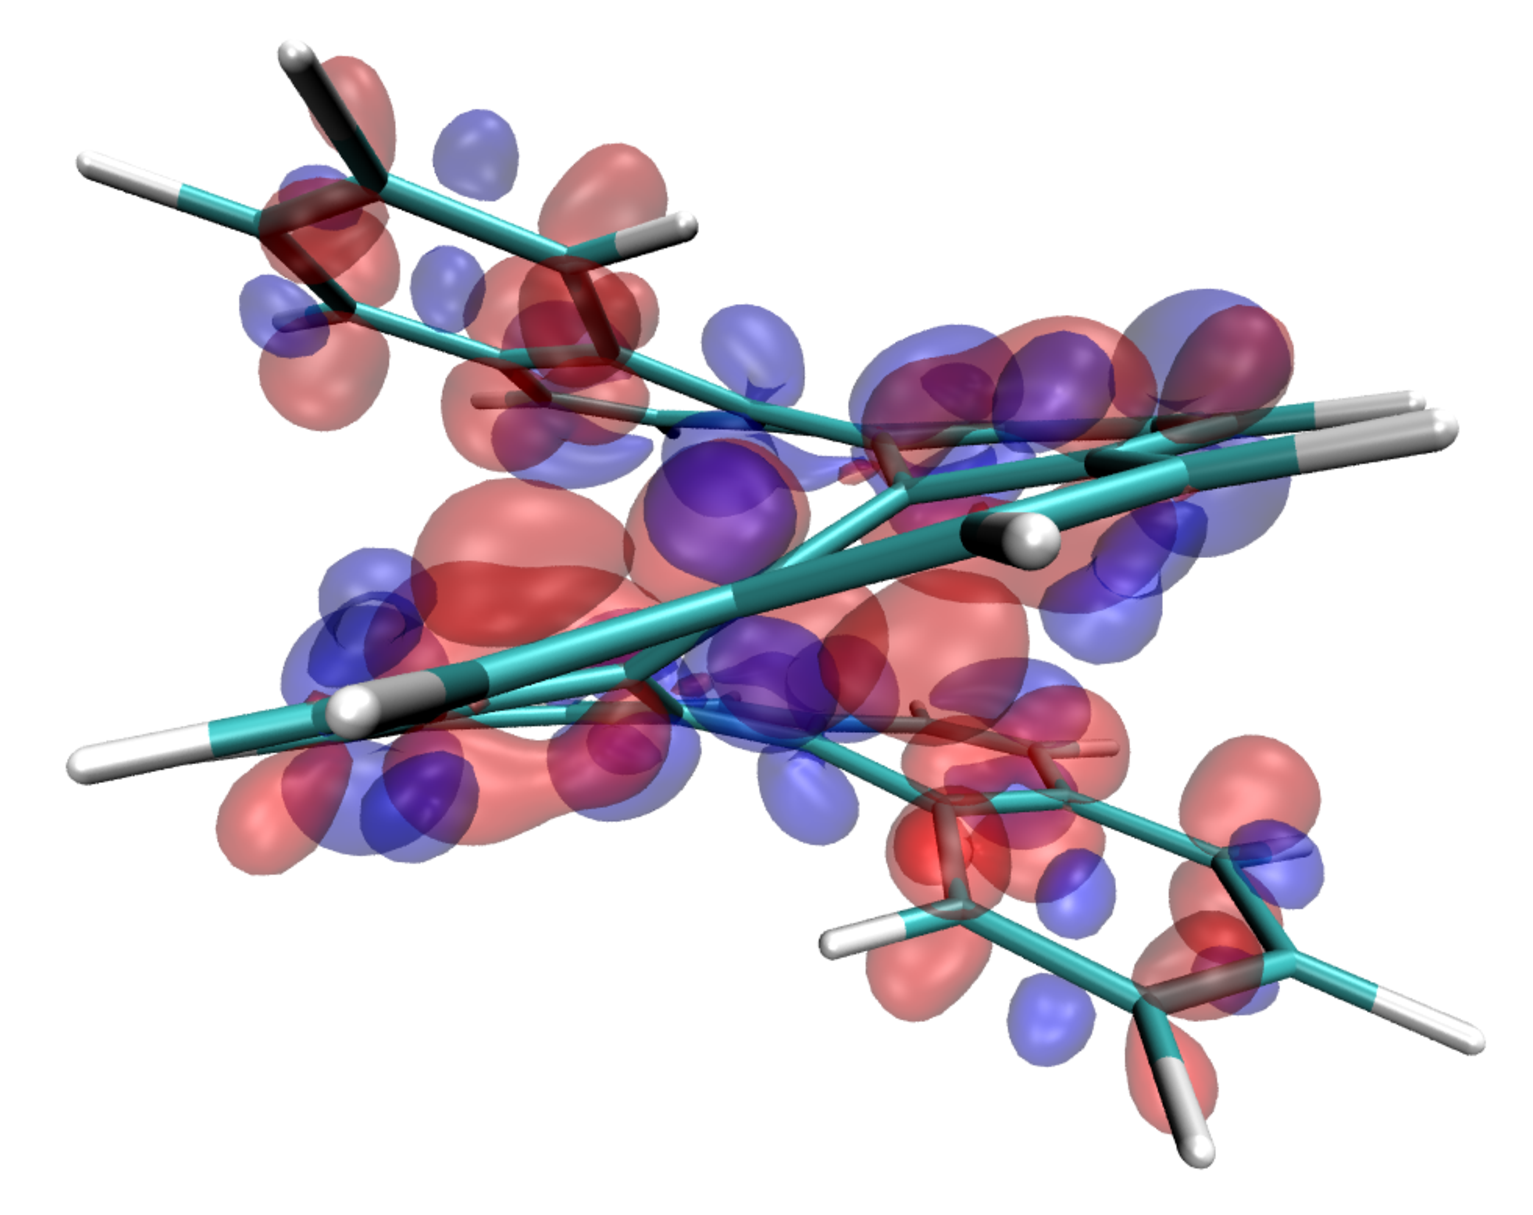
\includegraphics[width=4cm]{h10-pk1} &
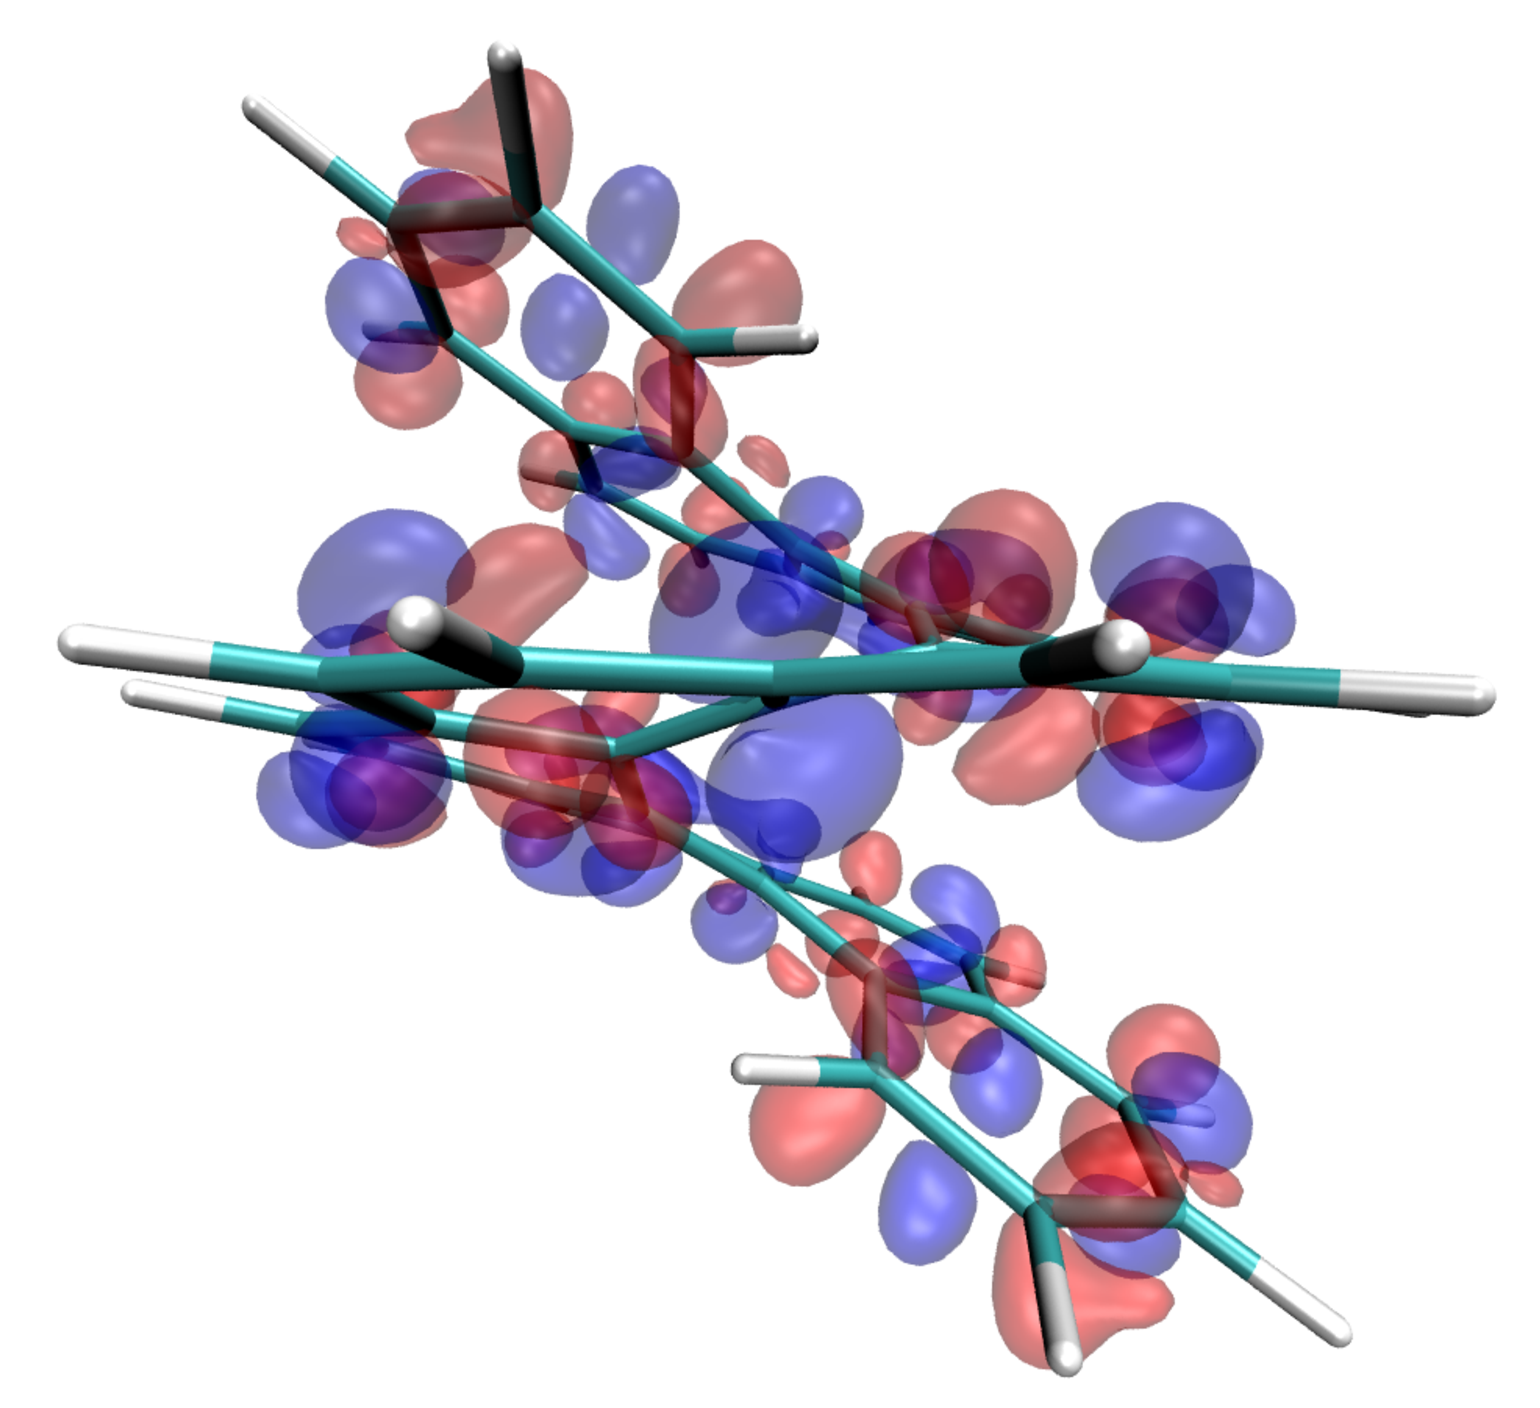
\includegraphics[width=4cm]{h10-pk2} \\
(a) 217~$nm$ & (b) 254~$nm$ \\
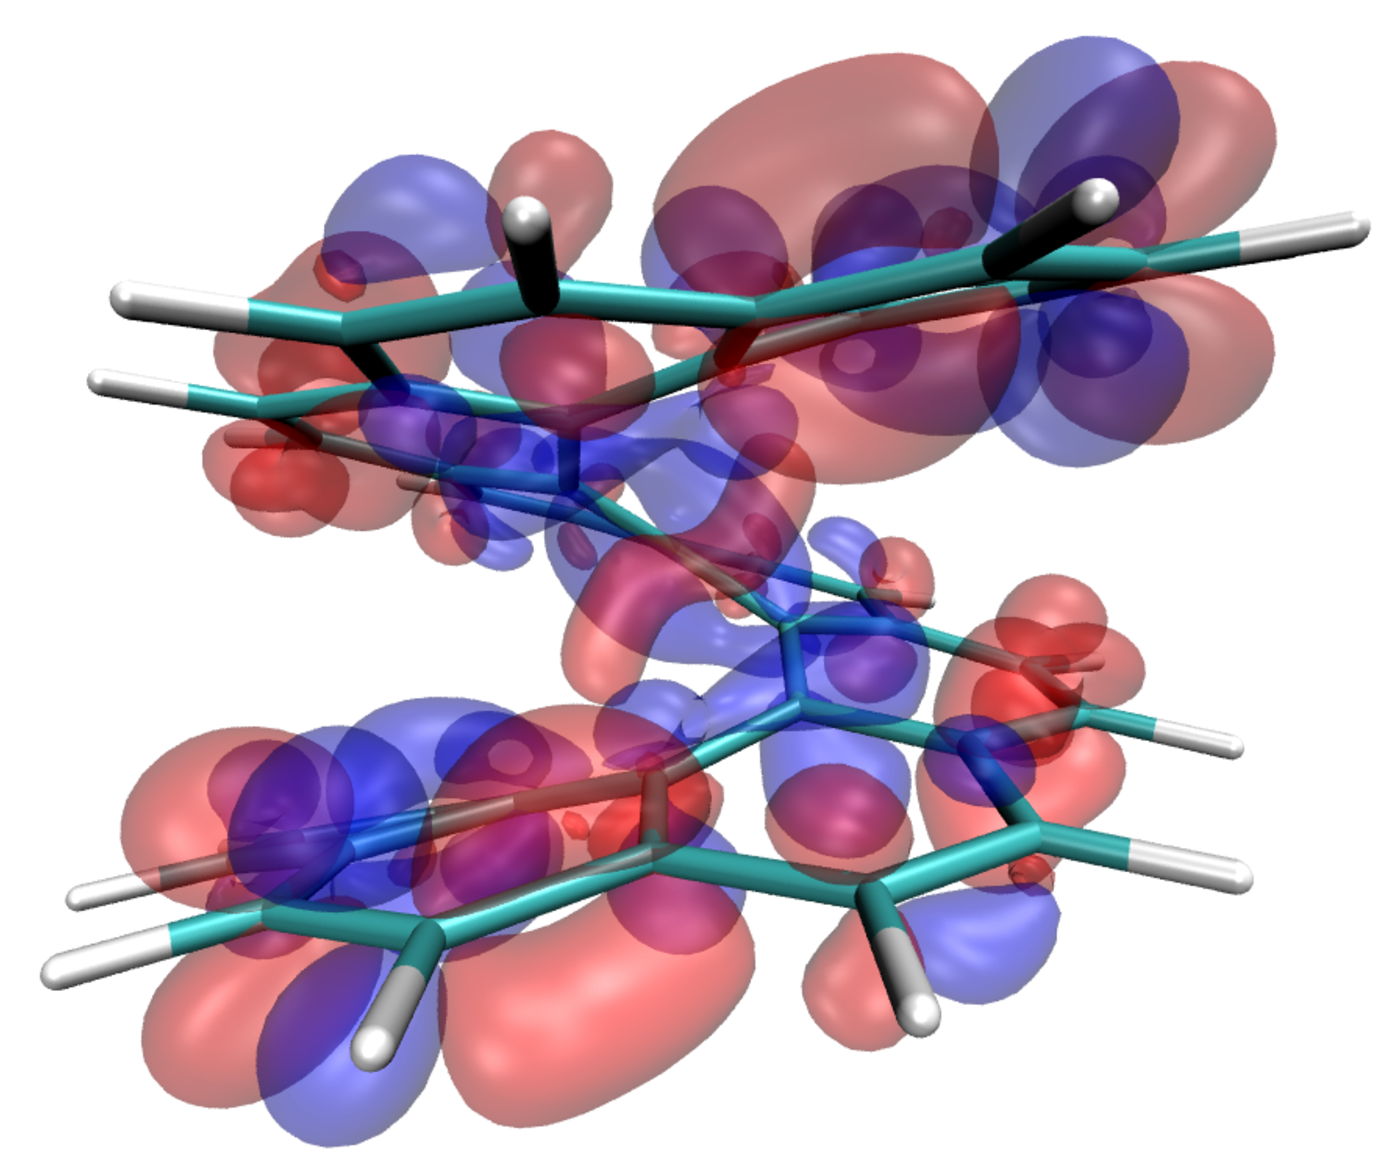
\includegraphics[width=4cm]{h10-pk3} &
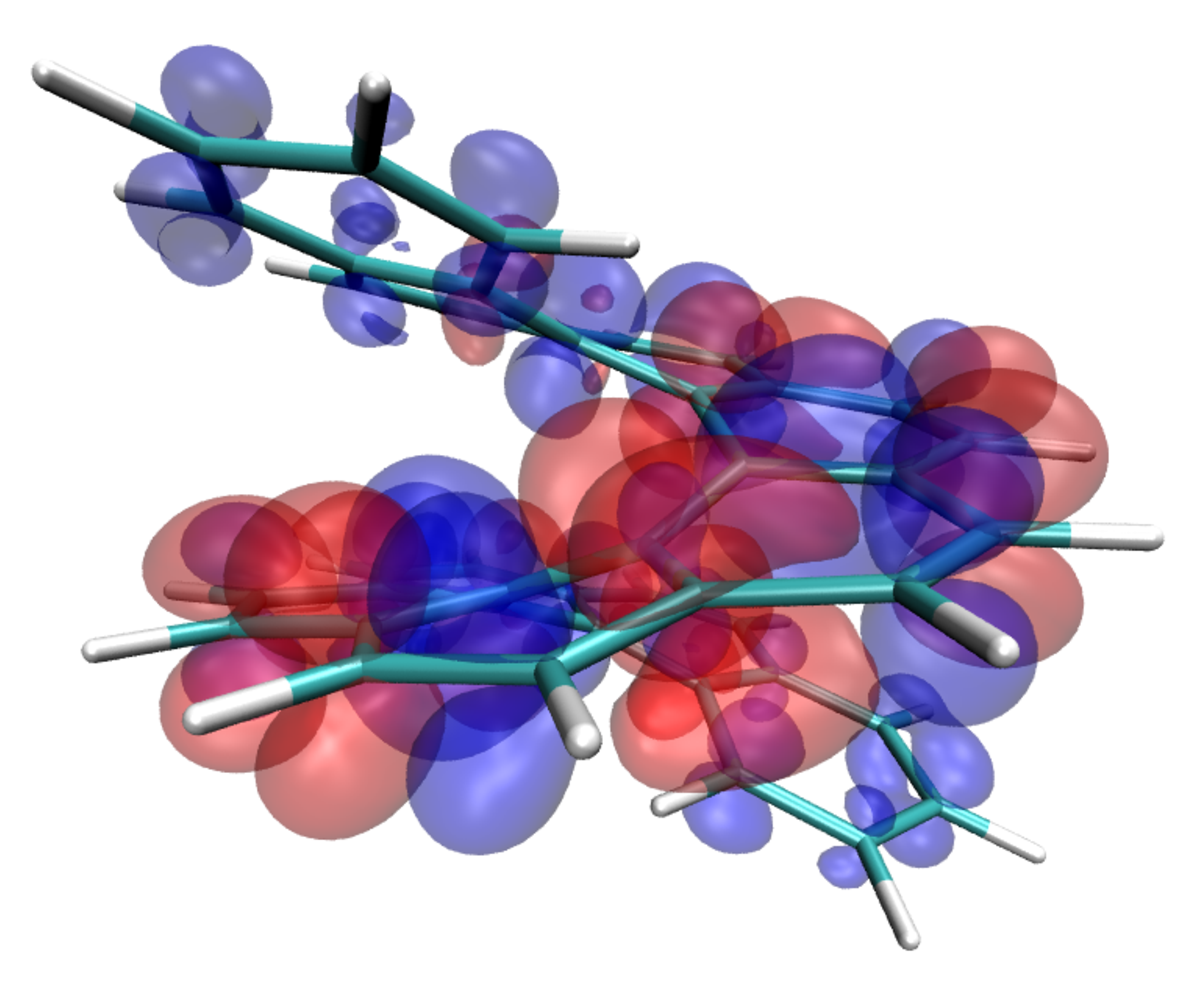
\includegraphics[width=4cm]{h10-pk4} \\
(c) 302~$nm$ & (d) 411~$nm$ \\
\end{tabular}
\caption[{[10]}helicene transition densities.]{Transition densities for [10]helicene. Excitations from left to right, top to bottom: (a) 217~$nm$, (b) 254~$nm$, (c) 302~$nm$, (d) 411~$nm$. In each case, the charge transfer is from the blue regions to the red. These are all-electron calculations performed at the TDDFT-PBE0 level.}\label{fig:helipeaks}
\end{figure}

Figure~\ref{fig:helipeaks} displays transition densities for the four most distinct peaks in the all-electron [10]helicene ECD spectrum. One sees that for all four, most of the electron density exhibits a strong $\pi$ character. The peak for which this is least true is the excitation at 302~$nm$, Figure~\ref{fig:helipeaks}c, which has a noticable degree of electron delocalisation around the centre of the helix. This may go some way to explaining why it is this particular peak that is least well-reproduced by the pseudopotentials, particularly $geom_1$.

\begin{figure}
\begin{tabular}{cc}
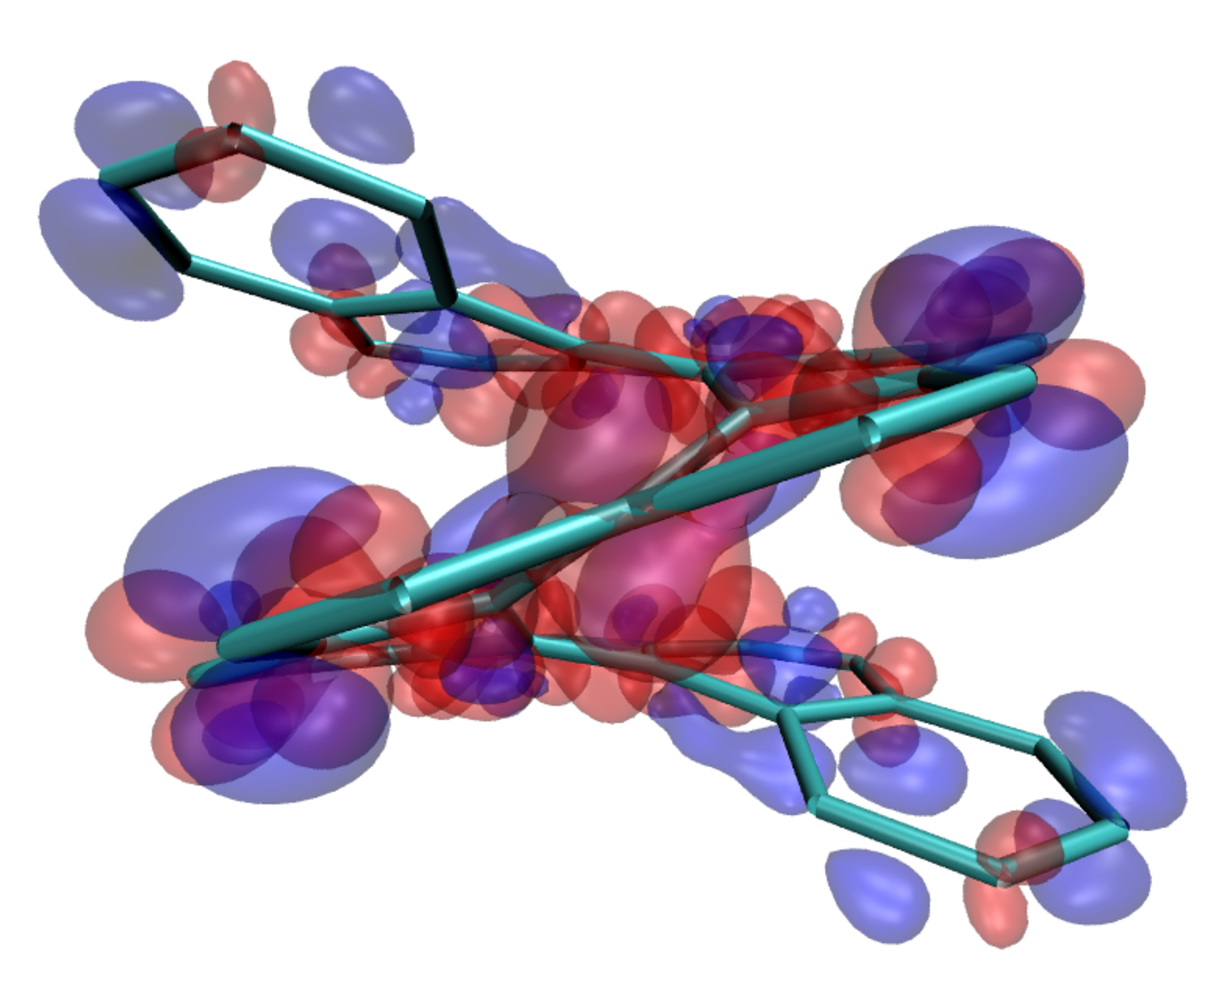
\includegraphics[width=4cm]{psh10-pk1} &
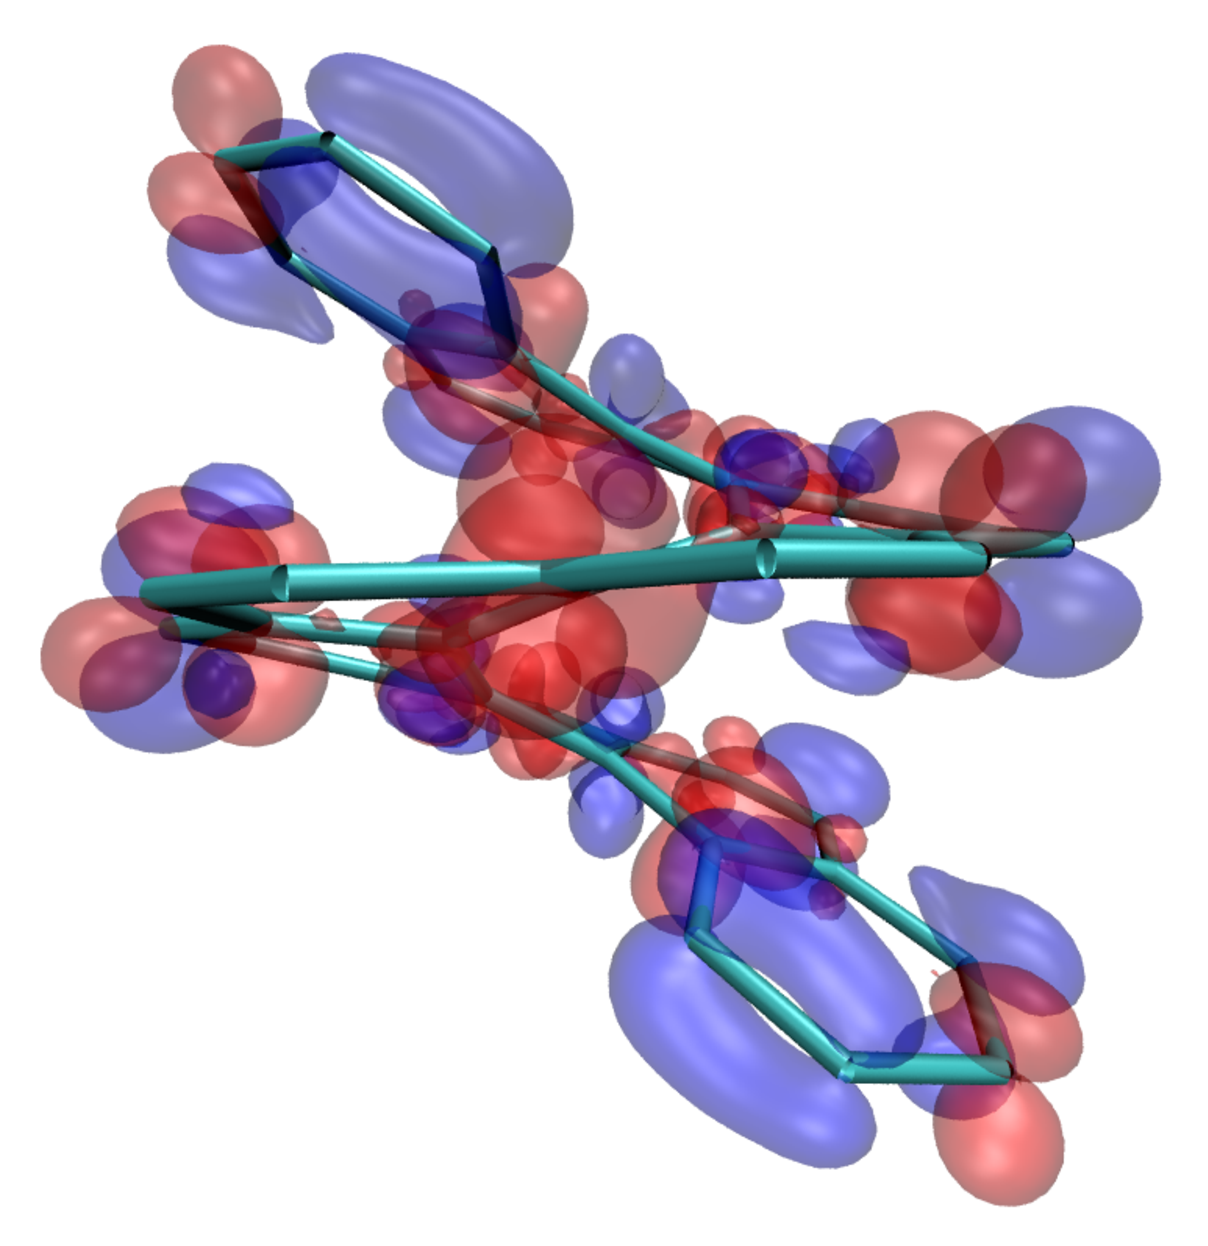
\includegraphics[width=4cm]{psh10-pk2} \\
(a) 217~$nm$ & (b) 250~$nm$ \\
\multicolumn{2}{c}{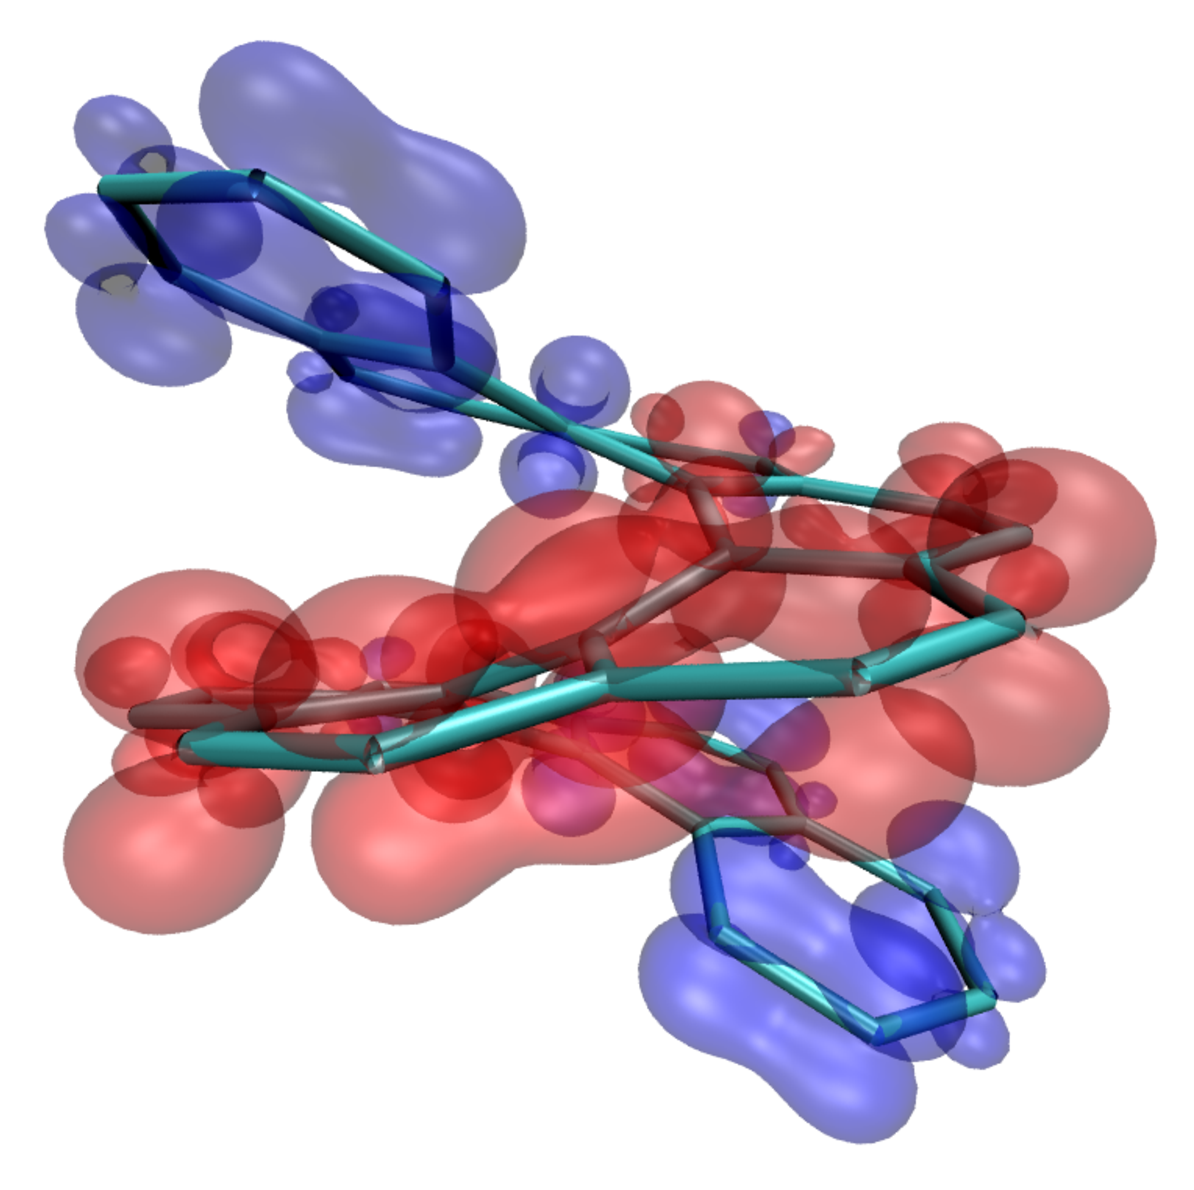
\includegraphics[width=4cm]{psh10-pk3}} \\
\multicolumn{2}{c}{(c) 423~$nm$}\\
\end{tabular}
\caption[$geom_1$ pseudo{[10]}helicene transition densities.]{Transition densities for pseudo[10]helicene using $geom_1$ pseudopotentials. Excitations from left to right, top to bottom: (a) 217~$nm$, (b) 250~$nm$, (c) 423~$nm$. In each case, the charge transfer is from the blue regions to the red. These calculations are performed at the TDDFT-PBE0 level.}\label{fig:pshelipeaks}
\end{figure}

Figure~\ref{fig:pshelipeaks} displays transition densities for $geom_1$ pseudo[10]helicene, for the three peaks which appear to line up best with those of the all-electron spectrum in Figure~\ref{fig:helispectrageom1}. Figures~\ref{fig:pshelipeaks}a, b and c therefore correspond to Figures~\ref{fig:helipeaks}a, b, and d respectively. While the shapes of the lobes do not align as neatly with the all-electron transition densities of Figure~\ref{fig:helipeaks} as transition densities for planar molecules (see Appendix~\ref{app:edens}), we see that the densities all correspond to transitions of similarly $\pi$-$\pi$-like character. A difference however, between the pseudosystem and all-electron transition densities is that while it was noted above that Figure~\ref{fig:helipeaks}c contained some delocalisation of the electron density in the centre of the helix, this is true for all of the pseudosystem transitions in Figure~\ref{fig:pshelipeaks}. It is possible therefore that the $\pi$ electrons are not tightly-enough bound by the pseudopotentials, allowing for a greater electron delocalisation than that permitted by the all-electron systems.

We suggest two further possible explanations for the degradation of the ECD spectra: (1) with $n > 6$, the ends of the helicene overlap more and more, resulting in a much more complex electronic structure, and (2) that as the helicene length increases the steric effects of the overlapping $\pi$ rings causes an increasing distortion of individual benzene rings, \emph{i.e.} the helicene `stretches'~\cite{rickhaus_2015}.

These spectra show that we can be confident that our potentials can retain much of the physics of complex $\pi$ systems, even allowing for some distortion of the molecular plane. Using the definition of dihedral torsion shown in Figure~\ref{fig:distortiondef}, [6]helicene has a maximum dihedral torsion-per-ring of 14$^{\circ}$, while for [10]helicene this figure is 16$^{\circ}$. These calculations show that the ECD spectra of helicenes are mainly due to the $\pi$-like electrons and that our pseudopotentials allow for the reproduction of properties which are much more difficult to reproduce than UV spectra as they are much more sensitive to the environment. We can also say that the $geom_1$ pseudopotentials prove to be more accurate than the $set4$ potentials for the reproduction of helicene spectra.

\begin{figure}
\begin{center}
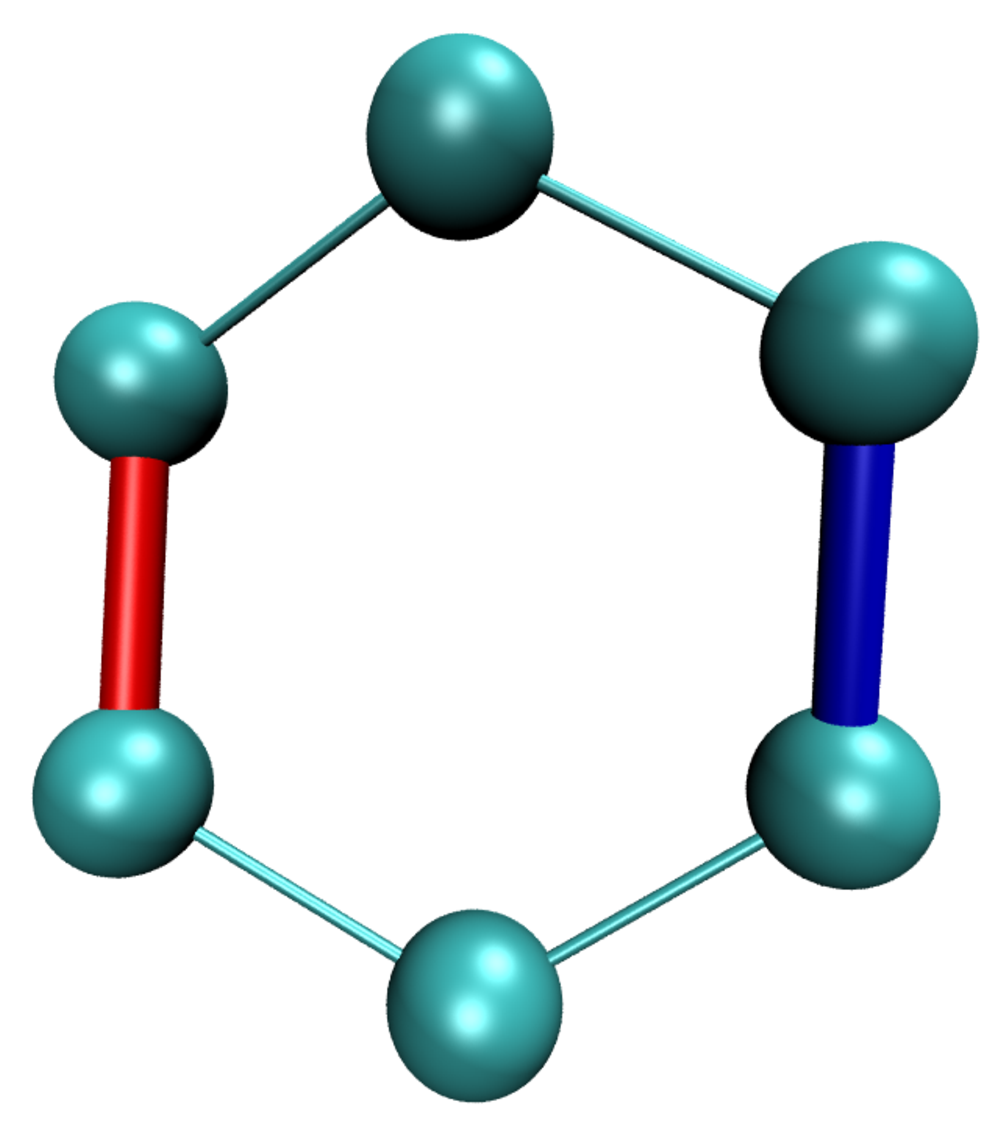
\includegraphics[height=3cm]{dihedraldef}
\hspace{2cm}
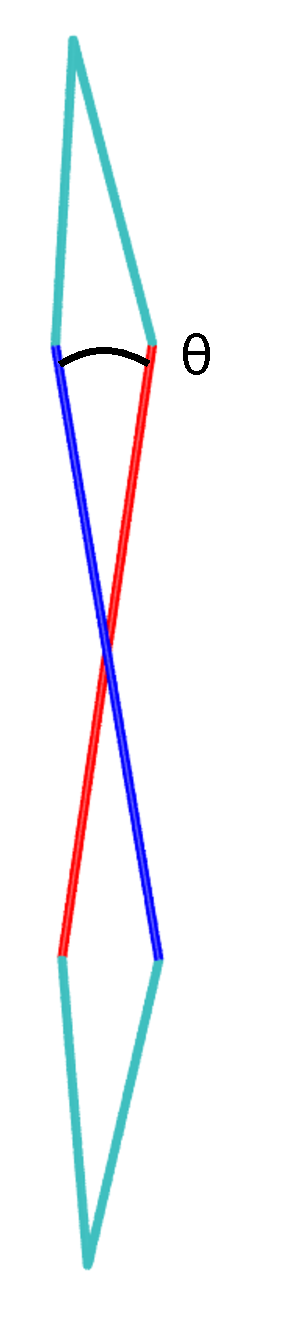
\includegraphics[height=3cm]{thiccerdihedral}
\end{center}
\caption[Definition of dihedral torsion for benzene]{Dihedral torsion of a benzene ring, viewed from the front (left) and the side (right). In this work, the dihedral torsion of an individual benzene ring is defined as the maximum angle $\theta$ between any two opposing bonds in the ring.}\label{fig:distortiondef}
\end{figure}

\subsection{Complex Spectra: Twistacene}
\label{sec:twistacene}

The phrase `twisted acene', later `twistacene', was introduced in 2004~\cite{lu_2004}, then more throroughly described in 2006~\cite{pascal_2006}. The electronic and optical properties of their parent acenes are altered by this twisting; notably, they are more soluble~\cite{xiao2012synthesis}. The twisting also introduces chirality to the molecule, and can produce bathochromic shifts~\cite{bedi_2018}. 

Study of these molecules is complicated by the fact that the twisting must be induced by other chemical fragments acting on the acene, making them hard to study directly. However, efforts have been made to study the electronic structure of twistacenes in a systematic manner, such as that of Bedi \emph{et al.}~\cite{bedi_2018}. In this paper, they describe a system  allowing them to `helically-lock' an acene at a specific torsion angle, and it is to this publication that we turn for geometric data. Figure~\ref{fig:tetheredanthracene} shows the Ant-c$n$ molecule (where $n$=3-6 is the length of the carbon bridge at the top of the molecule), which allows the helical locking of anthracene. The increasing length $n$ of the carbon bridge at the top of the molecule allows the anthracene to relax back toward a planar alignment.

\begin{figure}
\begin{center}
\begin{tabular}{c c}
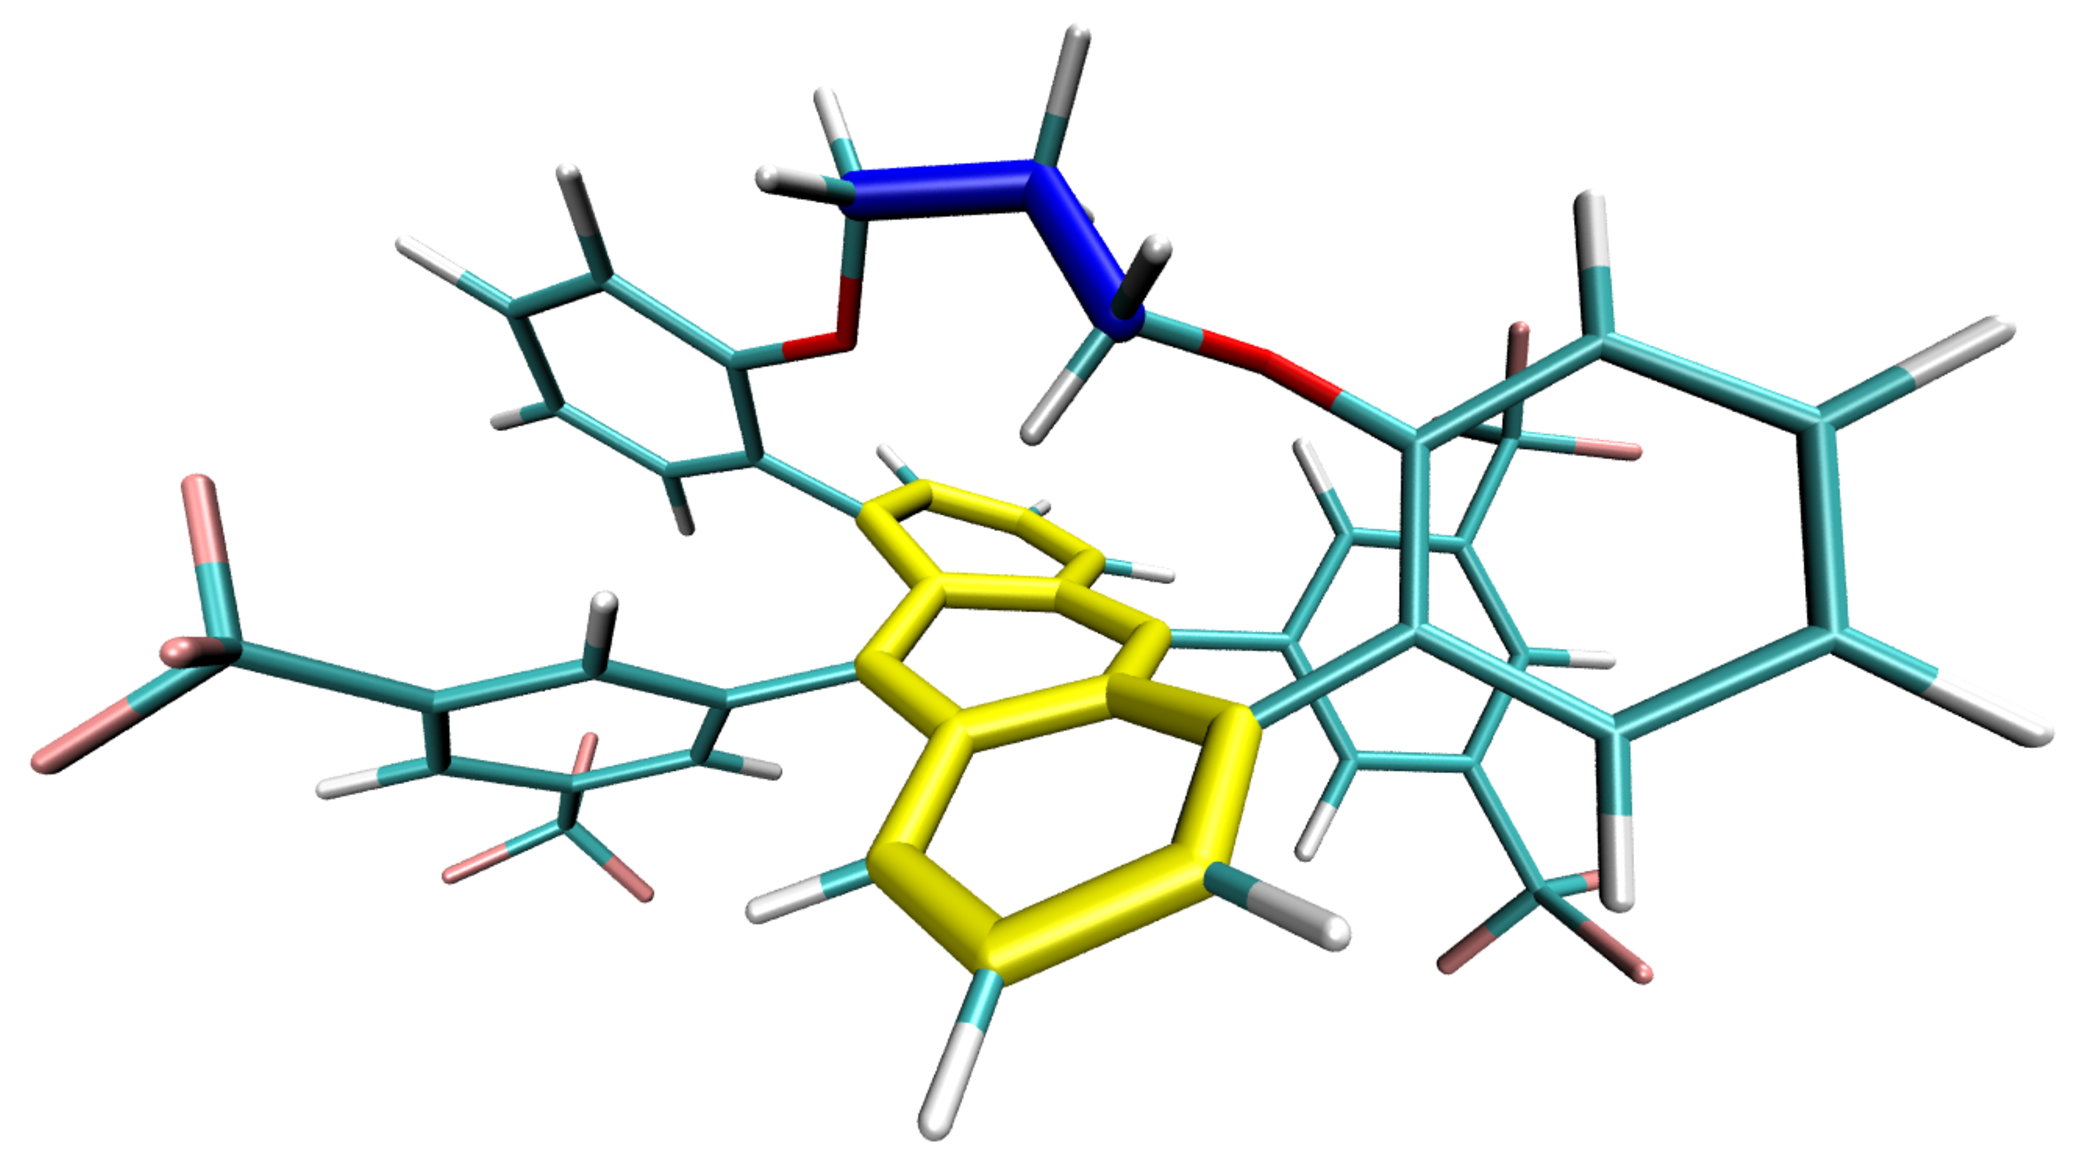
\includegraphics[width=4cm]{c3-highlights} & 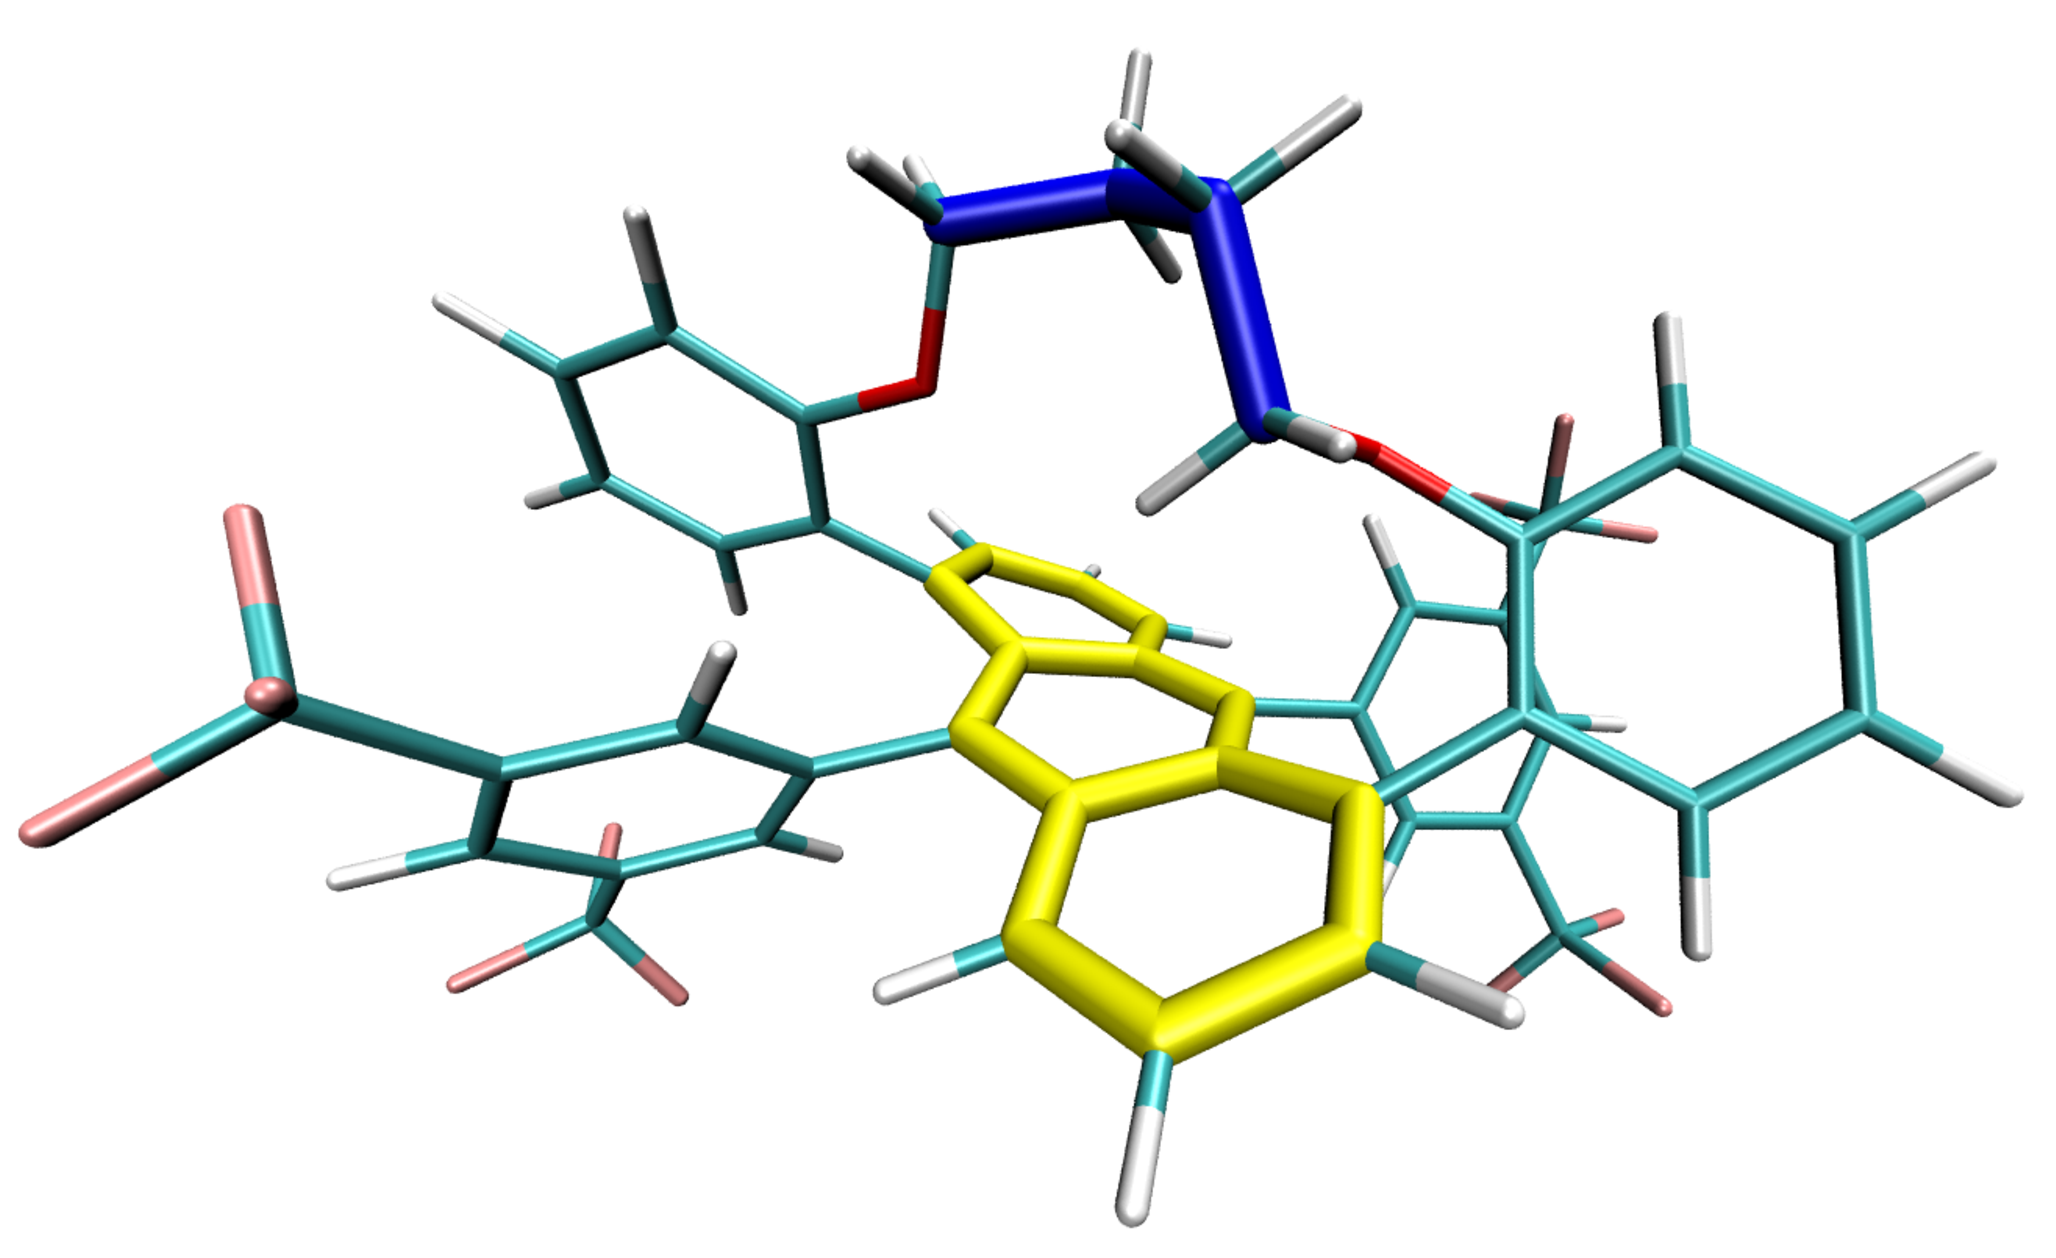
\includegraphics[width=4cm]{c4-highlights} \\
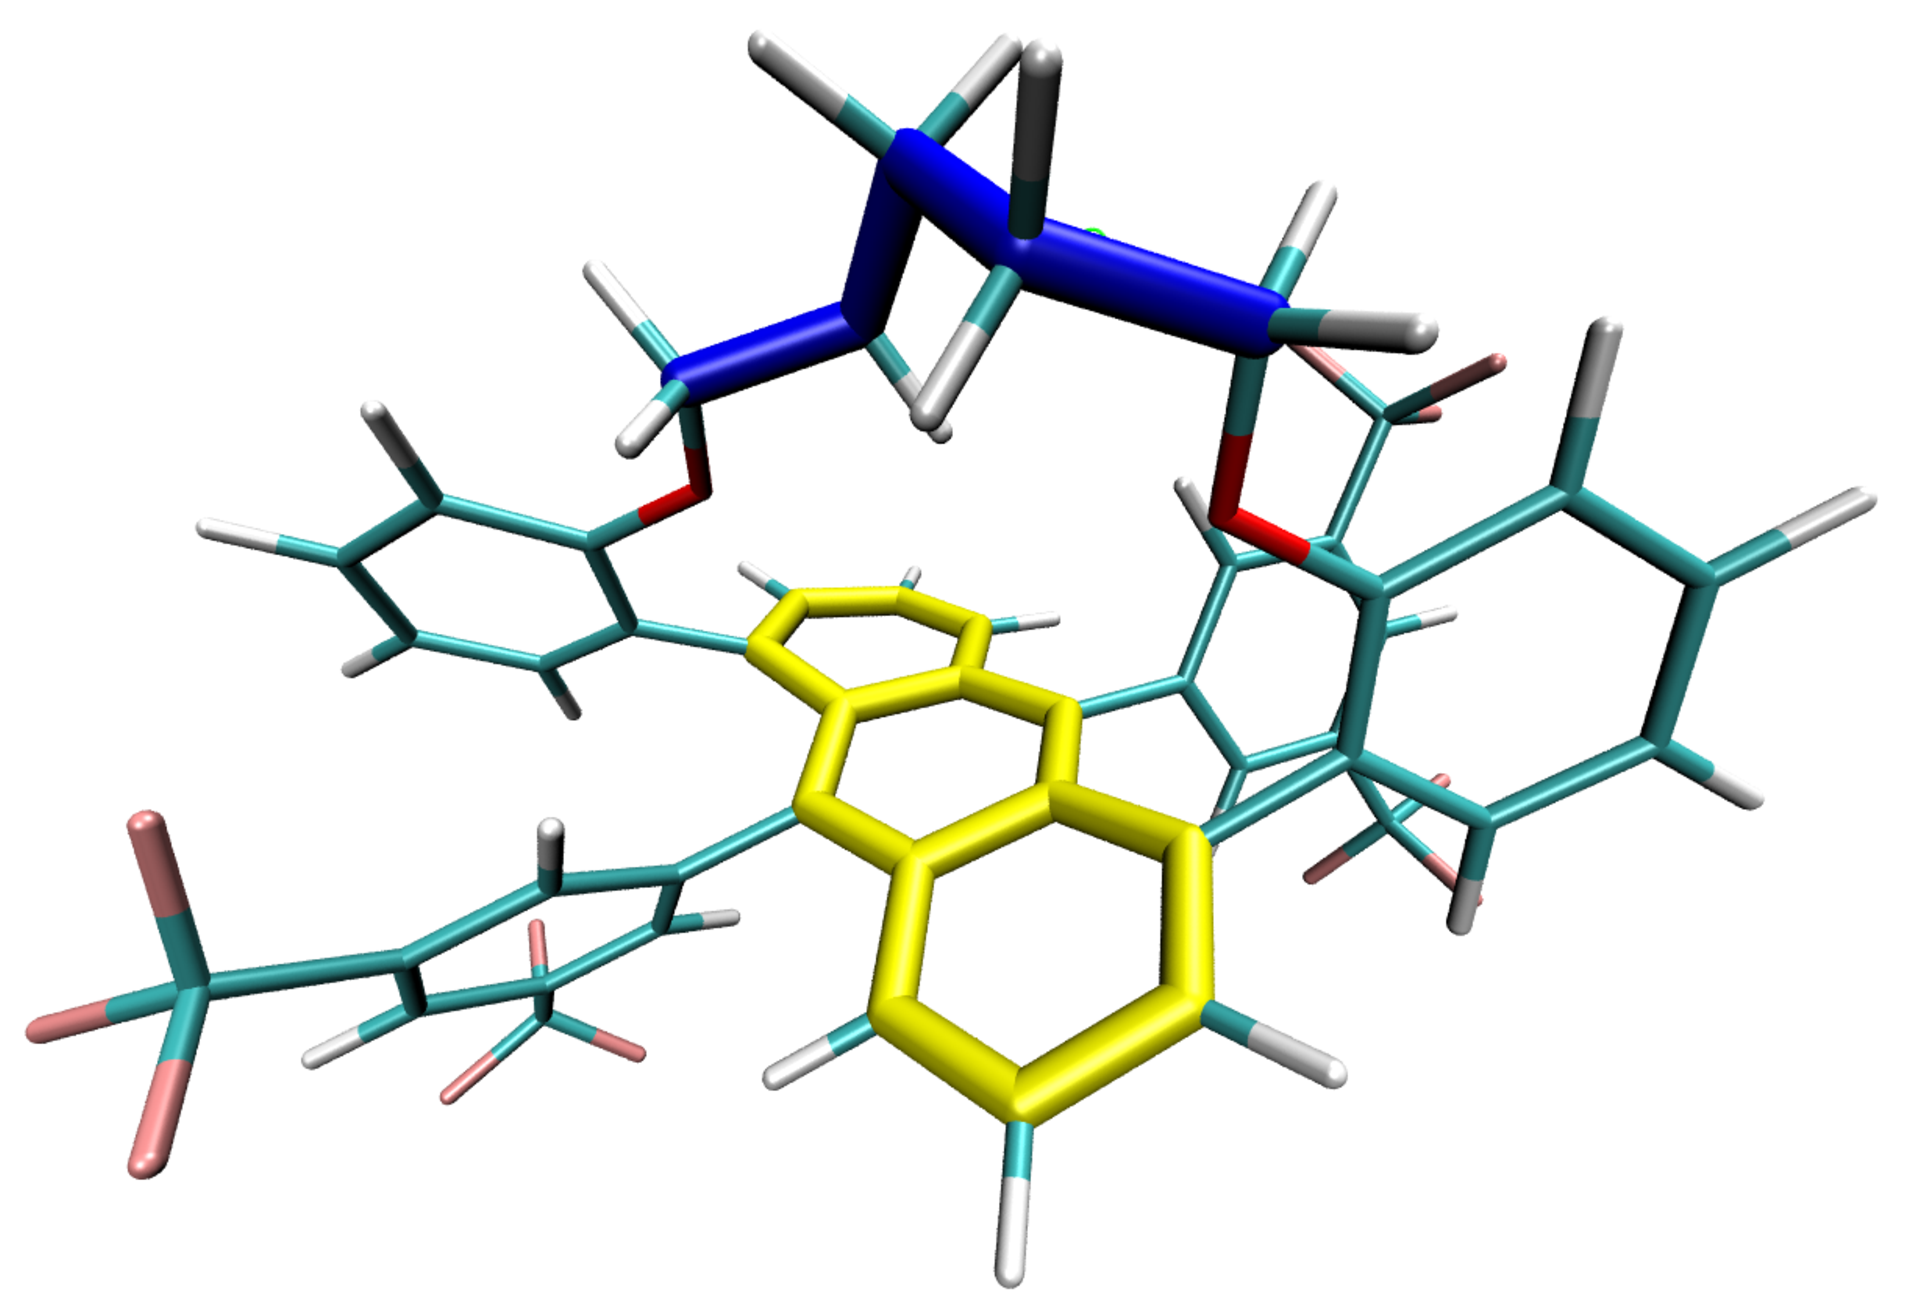
\includegraphics[width=4cm]{c5-highlights} &
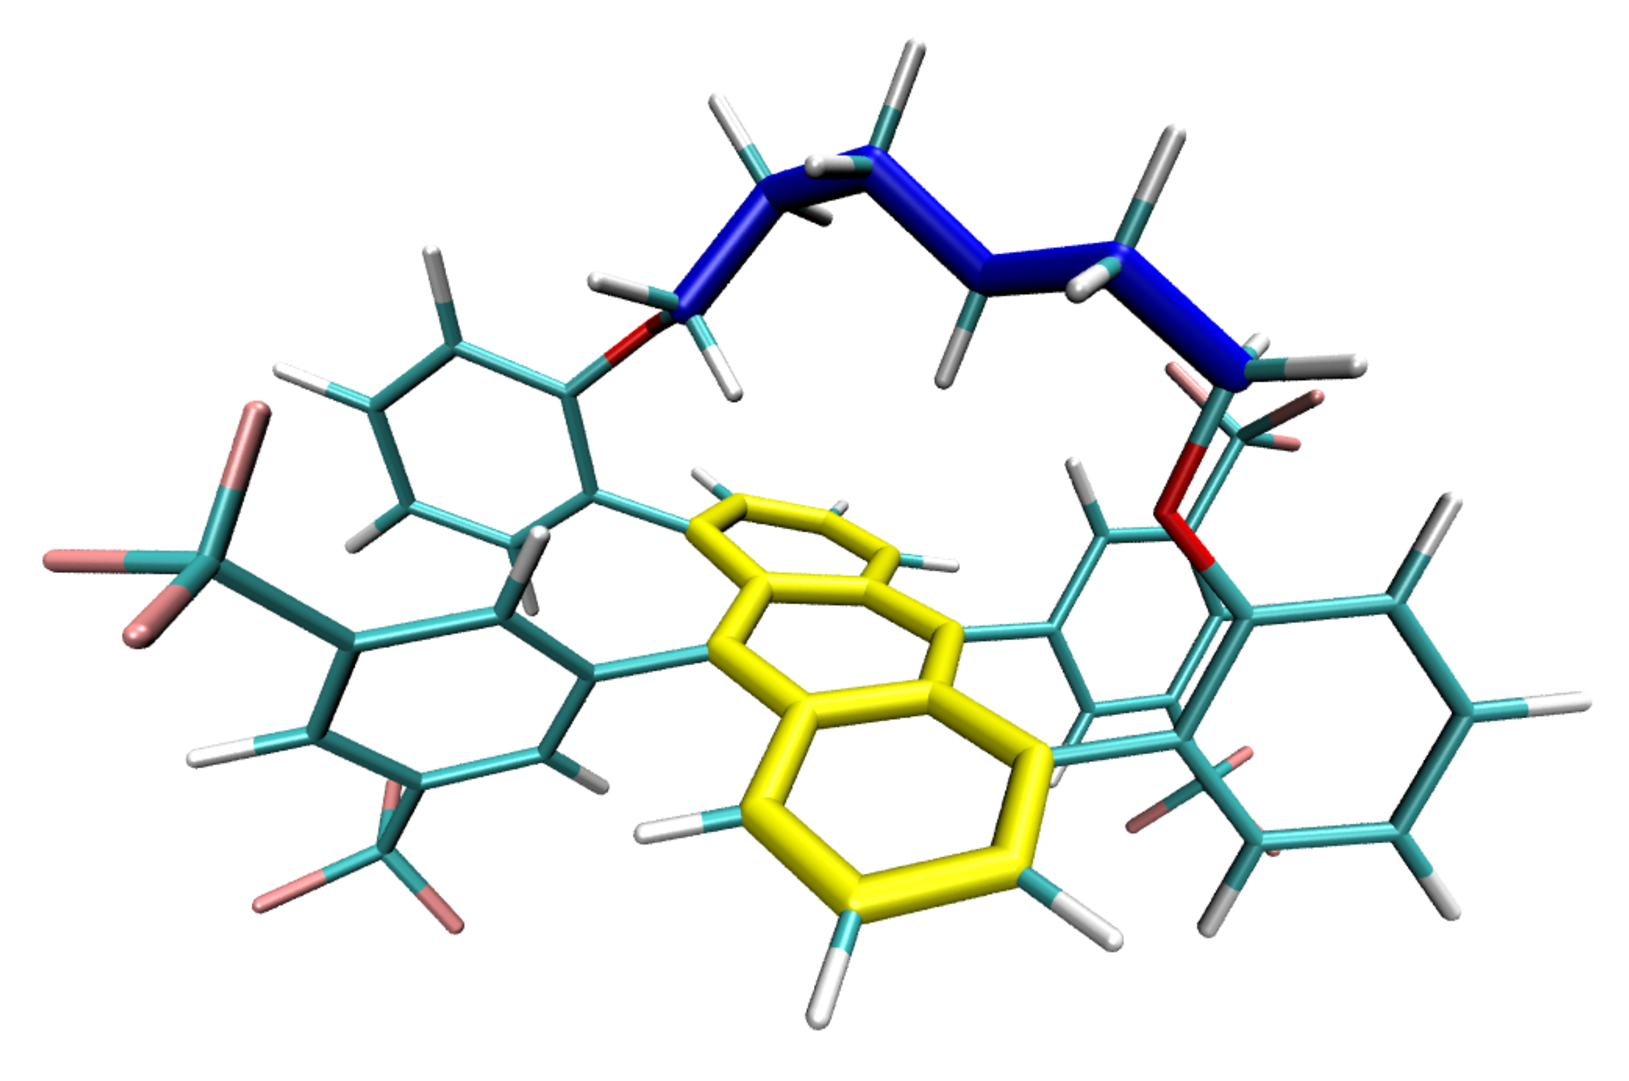
\includegraphics[width=4cm]{c6-highlights} \\
\end{tabular} 
\end{center}
\caption[Twistacene structure diagrams.]{Structures of Ant-c$n$, where $n=3-6$. From left to right and top to bottom: Ant-c3 (torsion angle 38$^{\circ}$), Ant-c4 (torsion angle 32$^{\circ}$), Ant-c5 (torsion angle 30$^{\circ}$), Ant-c6 (torsion angle 23$^{\circ}$). In each case, the anthracene itself is highlghted in yellow, while the carbon bridge that determines the torsion is highlighted in blue.}\label{fig:tetheredanthracene}
\end{figure}

This molecule is of specific interest to us for similar reasons to the helicene described in Section~\ref{sec:helicene}, \emph{i.e.} that the distorting of $\pi$ rings starts to break the separation of $\sigma$ and $\pi$ orbitals, which will in turn make our $\alpha$ potentials less and less physically descriptive of the system, likely leading to a poorer result. With a systematic test of increasingly distorted $\pi$ rings therefore, we can gain some idea of the limits of the pseudopotentials used.

\subsubsection{Results and Discussion}

As our interest was solely in the part of the molecule we wished to model with pseudopotentials, \emph{i.e.} the twisted anthracene itself, we first optimised the molecular geometries (at the DFT-PBE0 level, with def-SV(P) basis sets) before removing the atoms surrounding the central anthracene. This way, we could calculate the UV spectra without the risk of the anthracene peaks being obscured by excitations in parts of the molecule in which we were not interested.

\begin{figure}
\begin{center}
\includegraphics[width=8cm]{twistacene_spectra}
\end{center}
\caption[Twistacene all-electron and pseudopotential spectra.]{UV and ECD spectra for twisted anthracenes Ant-c$n$ (for $n=3-6$), calculated at the TDDFT-PBE0 level for the first 20 singlet excitations. These include the all-electron spectra (red), the $set4$ potential spectra (green), and the $geom_1$ potential spectra (blue).}\label{fig:antc_spectra}
\end{figure}

Figure~\ref{fig:antc_spectra} displays the spectra for Ant-c$n$, for $n=3-6$, using all-electron structures as well as two different sets of pseudopotentials, the original $set4$ potentials, and also the $geom_1$ set. The all-electron UV spectra are very similar to one another and have peaks in approximately the 120~$nm$ to 400~$nm$ range, with most of the peaks clustered between roughly 120~$nm$ and 280~$nm$, and the main peak at around 240~$nm$ in each molecule. Both of the pseudopotential sets reproduce the broad shape of the all-electron spectra, though both have an extra cluster of peaks at the high end of the spectra in the 100-150~$nm$ range. This is likely due to the phenomenon noted in Section~\ref{sec:spectraloptimisation}, whereby calculating $n$ excitations in a pseudopotential and an all-electron system will result in more higher-energy peaks in the pseudosystem, due to excitations that are possible in the all-electron system being prevented in the pseudosystem by the missing electrons. For both sets of potentials, the majority of the peaks in the all-electron systems appear to be present in the pseudosystems, though it is hard to see exactly which pseudopotential peaks correspond to the lowest-energy peak in the all-electron spectra at around 380~$nm$. The relative intensities of the peaks also seem broadly correct. The pseudopotential sets differ in that the $geom_1$ set has a much smaller relative shift that the $set4$ set. The main peak is shifted by around 20~$nm$ for $geom_1$, but by around 50~$nm$ for $set4$. This is in keeping with the spectral earlier results for $geom_1$ and $set4$ for ring molecules.

\begin{figure}
\begin{center}
\includegraphics[width=8cm]{twistacene_spectra_zoom}
\end{center}
\caption[Zoomed twistacene all-electron and $geom_1$ ECD spectra.]{A close up of Figure~\ref{fig:antc_spectra}, showing only ECD spectra for all-electron (red) and $geom_1$ (blue) calculations for  Ant-c$n$ (for $n=3-6$).}\label{fig:antc_spectra_zoom}
\end{figure}

Turning to the ECD results, we see a very different picture. The $geom_1$ potential spectra peaks are once more in a similar range of frequencies to that of the all-electron spectra (while the $set4$ potential spectra have a large and broad peak in the 400-600~$nm$ range not present in either of the other sets of spectra), but beyond that it is hard to compare them. We see that the pseudopotential spectra differ greatly from each other, as well as from the all-electron spectrum, and there are few consistently identifiable peaks, other than perhaps the negative peak at around 180~$nm$, which seems to be present in all three spectra across all molecules. It does not seem possible even to identify the broad positive-to-negative or negative-to-positive shift characteristic of chiral molecules. One curious feature of these spectra however, is that the pseudosystem spectra seem to accord slightly better to the all-electron spectra as the systems become more distorted, whereas intuition would suggest the opposite, that the pseudopotentials would become more unphysical as the system became more distorted and the $\sigma$-$\pi$ separation broke down. Figure~\ref{fig:antc_spectra_zoom} displays a closer comparison of all-electron and $geom_1$ ECD spectra in the 120 to 260~$nm$ range, in which the only consistently-identifiable peak appears to be that at around 180~$nm$ in all Ant-c$n$. Another noticeable feature of these ECD results is that both pseudopotential spectra produce peaks of a much higher relative intensity to those of the all-electron spectra.

This result seems inconsistent with the helicene results of Section~\ref{sec:helicene}. Table~\ref{fig:distortionangles} shows the maximum and mean distortion angles per benzene unit (see Figure~\ref{fig:distortiondef}) across both helicene and twistacene molecules used in this work. Both maximum and average distortion rates ber benzene unit are only greater for twistacene than for anthracene in the cases of Ant-c3 and Ant-c4. For Ant-c5 and Ant-c6 the maximum distortion rates are lower than those of all the helicene molecules, and the mean distortion of Ant-c5 and Ant-c6 is also mostly lower than those of the helicenes. Why then are the ECD spectra of helicene reproduced very well by the pseudopotentials, while those of twistacene are not? 

\begin{table}
\caption[Planar distortion of benzene compared to helicene.]{Maximum and mean distortions per benzene unit for helicene and twistacene molecules used in this work. The maximum distortion per benzene unit is chosen to be the largest dihedral torsion angle in the molecule (see Figure~\ref{fig:distortiondef}).} \label{fig:distortionangles}
\begin{center}
\begin{tabular}{|c|.|.|}
\hline
\textbf{System} & \multicolumn{2}{|c|}{\textbf{Distortion ($^{\circ}$)}} \\
& \multicolumn{1}{|c|}{\textbf{Mean}} & \multicolumn{1}{|c|}{\textbf{Maximum}} \\
\hline
{[6]}helicene & 9.3 & 14.5 \\
{[7]}helicene & 10.7 & 15.6 \\
{[8]}helicene & 11.1 & 15.5 \\
{[9]}helicene & 11.5 & 15.7 \\
{[10]}helicene & 12.0 & 15.9 \\
Ant-c3 & 14.1 & 17.9 \\
Ant-c4 & 13.6 & 16.9 \\
Ant-c5 & 10.4 & 13.3 \\
Ant-c6 & 6.2 & 8.1 \\
\hline
\end{tabular}
\end{center}
\end{table}

Figure~\ref{fig:twistapeaks} displays transition densities for the five most distinct peaks in the all-electron Ant-c3 ECD spectrum. The first peak, Figure~\ref{fig:twistapeaks}a, at 159~$nm$ is one which is not reproduced at all by the pseudopotentials. The transition density shows us why this might be. It shows a strong $\sigma$ character, which the pseudomolecule will of course not be able to capture. The next two peaks, Figures~\ref{fig:twistapeaks}b and \ref{fig:twistapeaks}c, at 179~$nm$ and 217~$nm$, are of a much more $\pi$-like character, which explains why they can be identified in the Ant-c3 pseudomolecular spectra, though not why this should be the case for Ant-c3, the most distorted system, and not for the other, less-distorted anthracenes. The transition densities don't give a wholly satisfactory explanation for the other peaks, either. Neither the fourth nor fifth peaks, Figures~\ref{fig:twistapeaks}d and \ref{fig:twistapeaks}e, at 250~$nm$ and 385~$nm$ are accurately captured by either set of pseudopotentials, despite appearing to consist mostly of electron density transfer between $\pi$-like orbitals.

\begin{figure}
\begin{tabular}{cc}
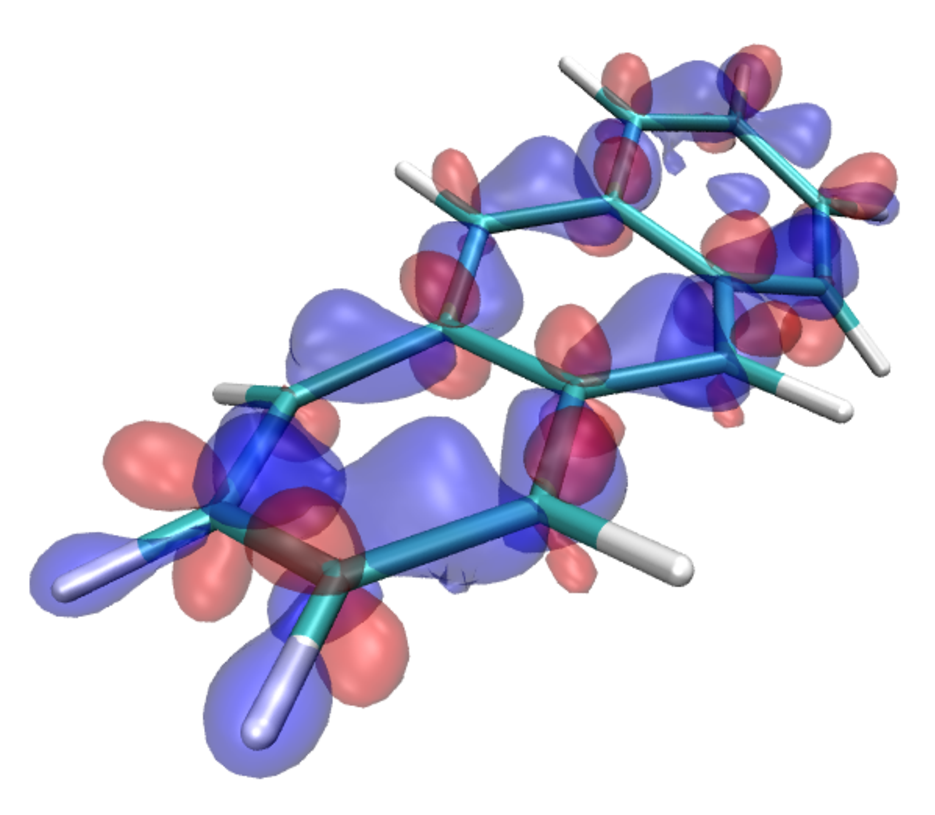
\includegraphics[width=4cm]{c3-pk1} &
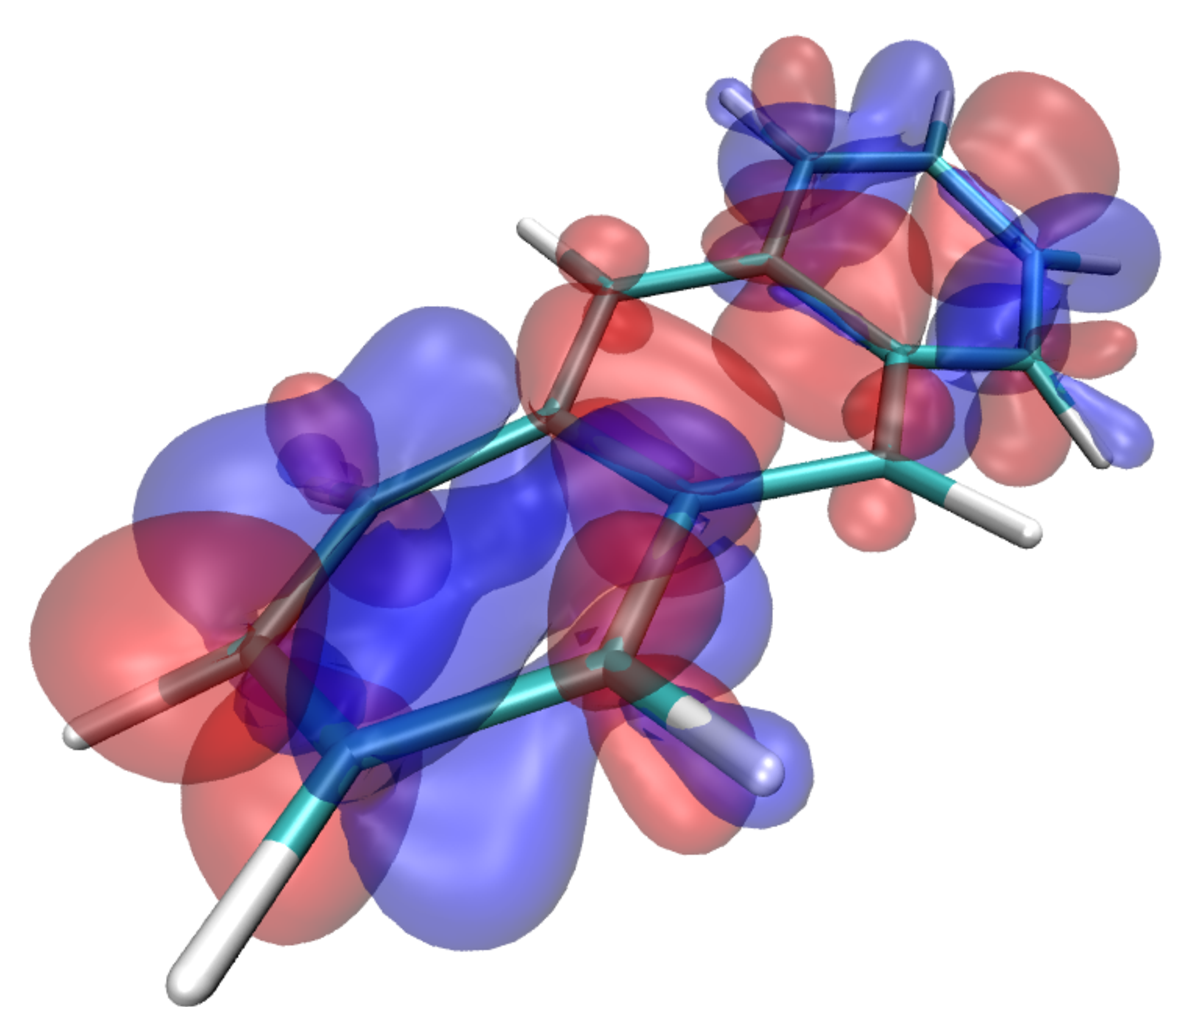
\includegraphics[width=4cm]{c3-pk2} \\
(a) 159~$nm$ & (b) 179~$nm$ \\
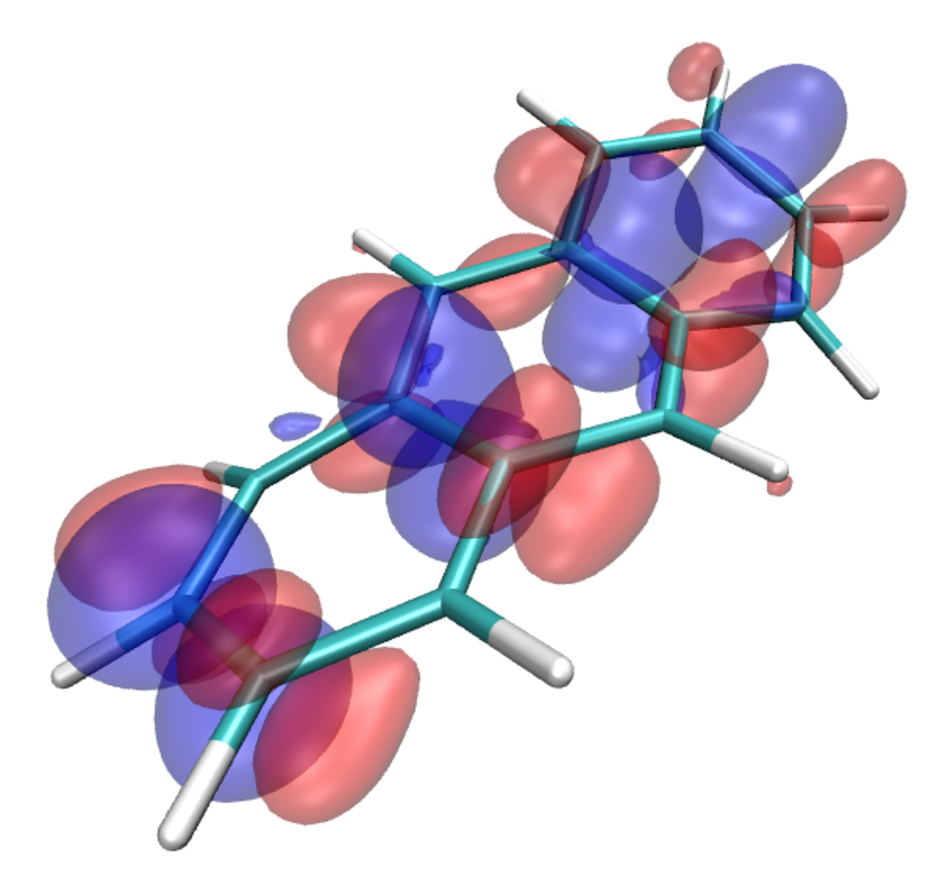
\includegraphics[width=4cm]{c3-pk3} &
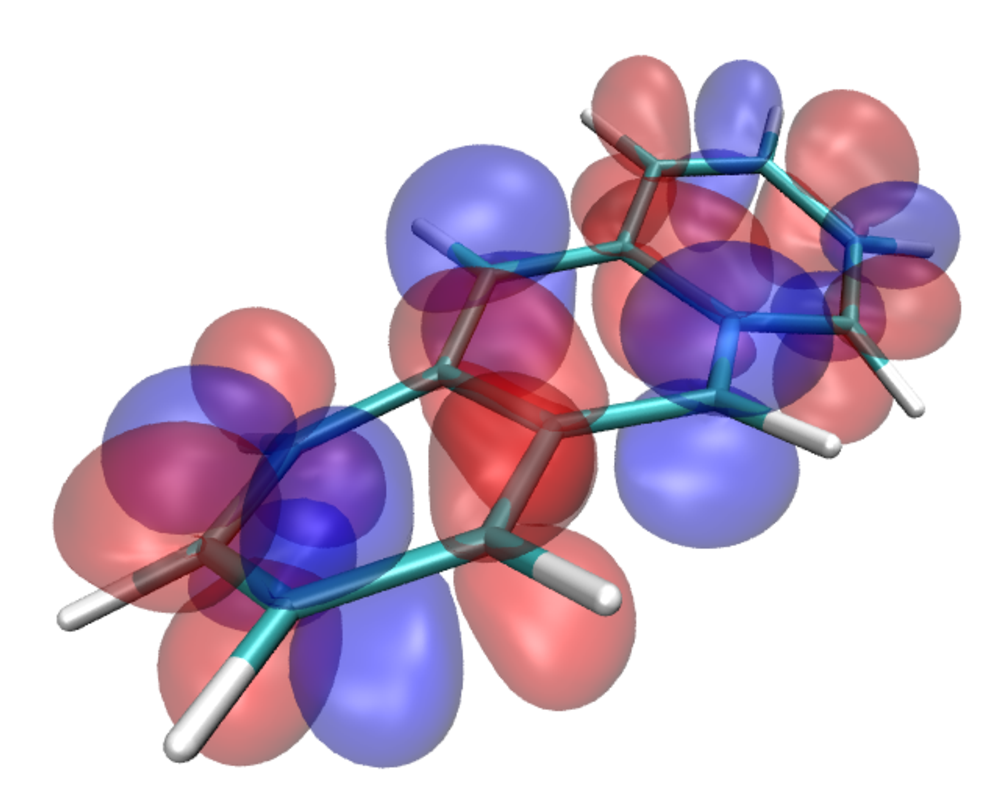
\includegraphics[width=4cm]{c3-pk4} \\
(c) 217~$nm$ & (d) 250~$nm$ \\
\multicolumn{2}{c}{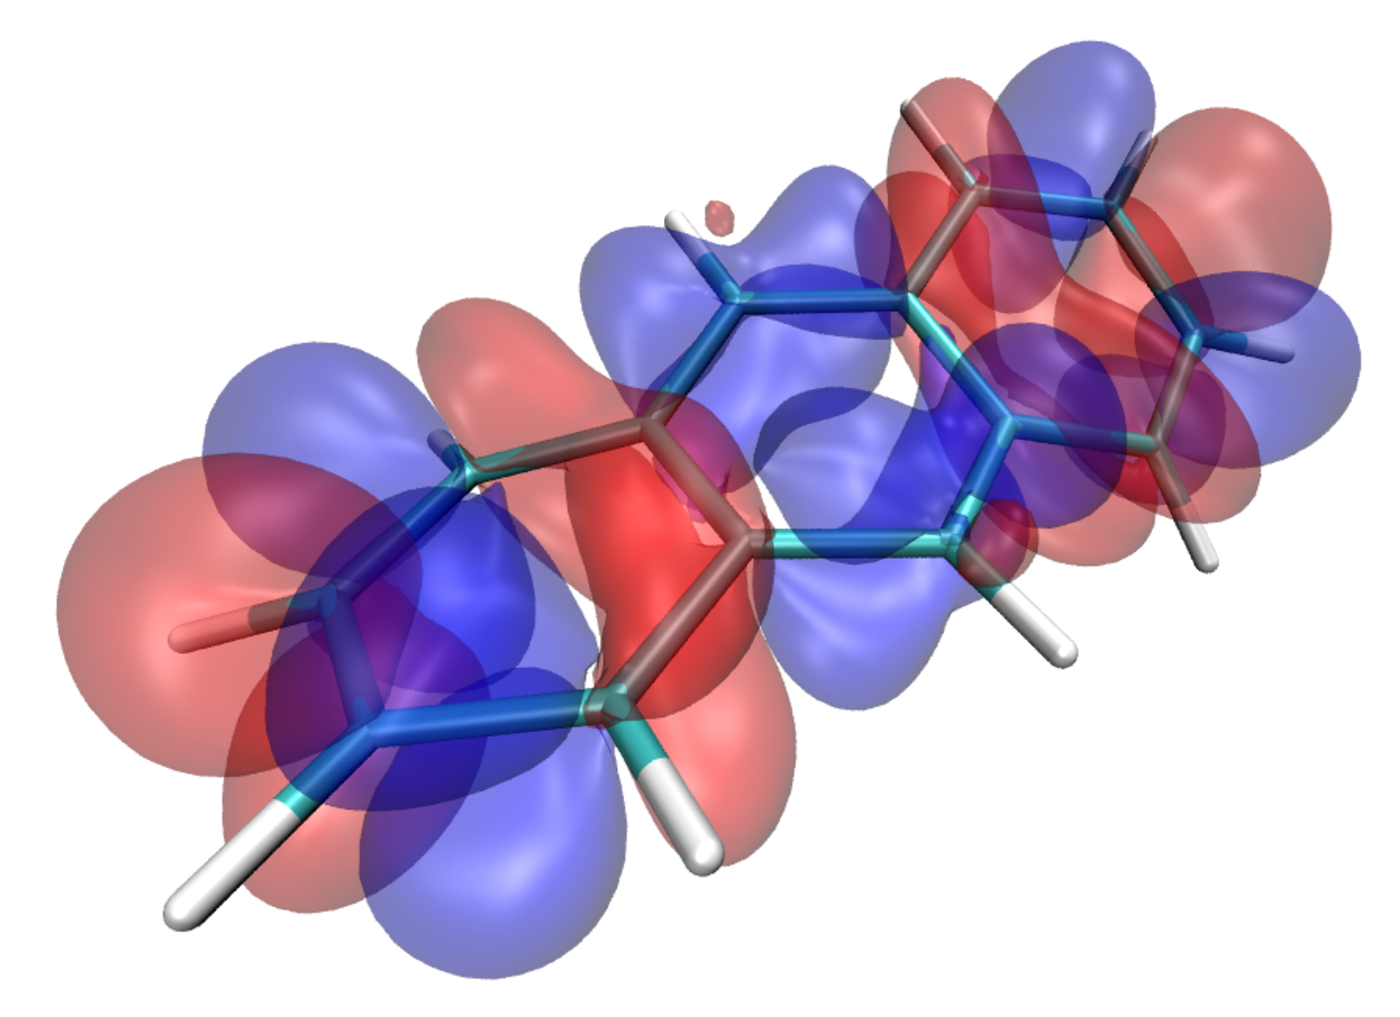
\includegraphics[width=4cm]{c3-pk5}}\\
\multicolumn{2}{c}{(e) 385~$nm$}\\
\end{tabular}
\caption[Transition densities for twistacene.]{Transition densities for Ant-c3. Excitations from left to right, top to bottom: (a) 159~$nm$, (b) 179~$nm$, (c) 217~$nm$, (d) 250~$nm$, (e) 385~$nm$. In each case, the charge transfer is from the blue regions to the red. These are all-electron calculations performed at the TDDFT-PBE0 level.}\label{fig:twistapeaks}
\end{figure}

\begin{figure}
\begin{tabular}{cc}
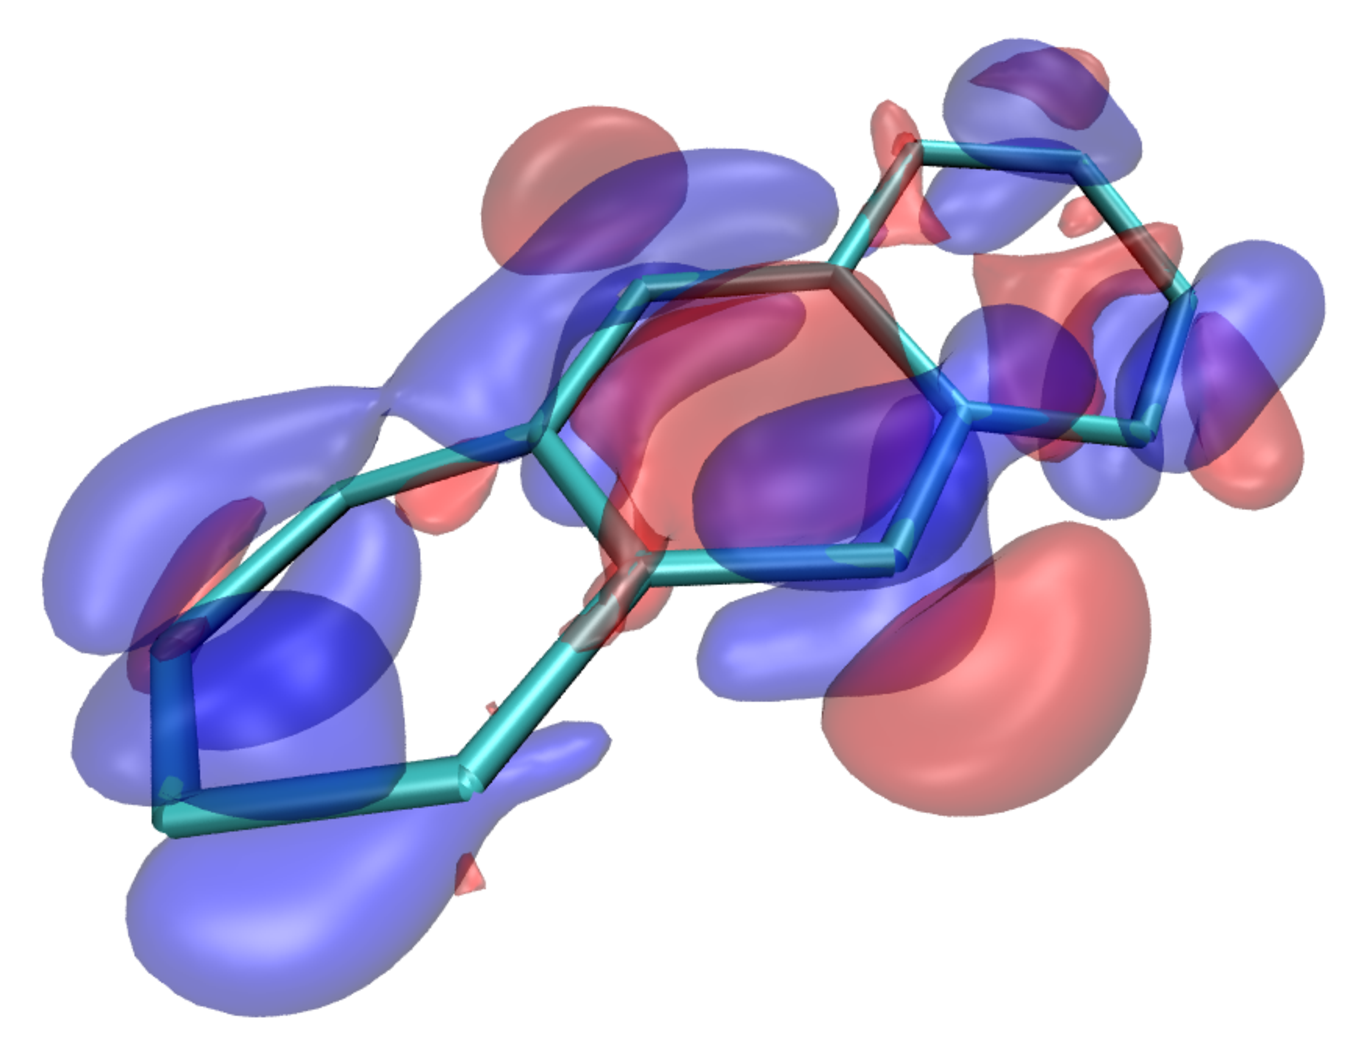
\includegraphics[width=4cm]{psc3-pk1} &
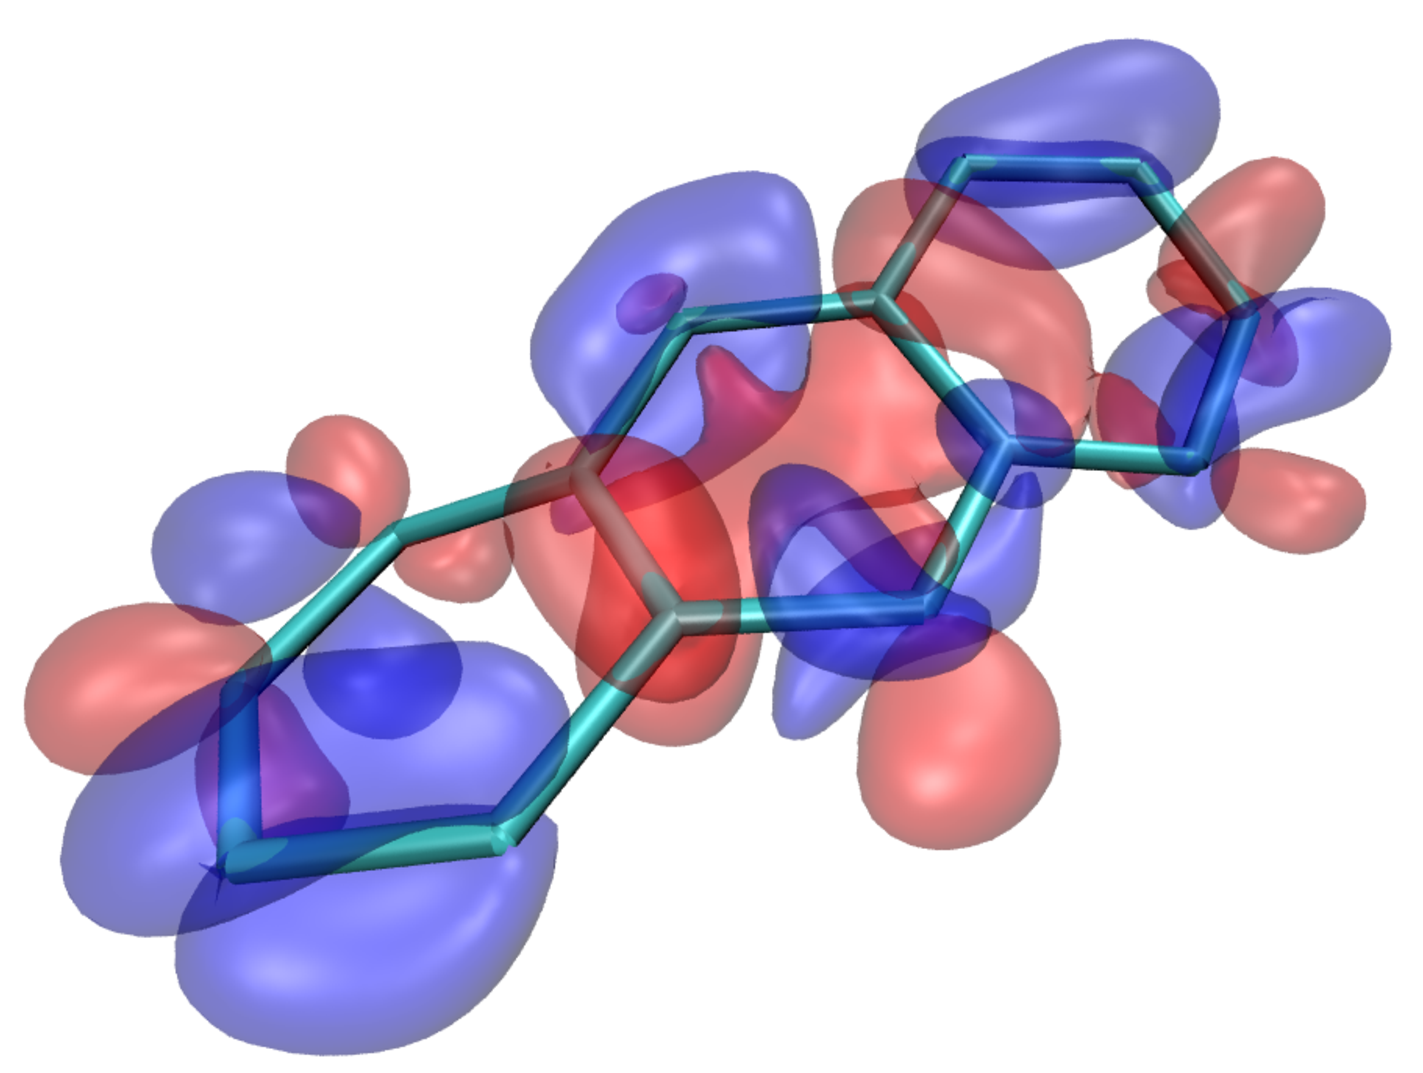
\includegraphics[width=4cm]{psc3-pk2} \\
(a) 153~$nm$ & (b) 177~$nm$ \\
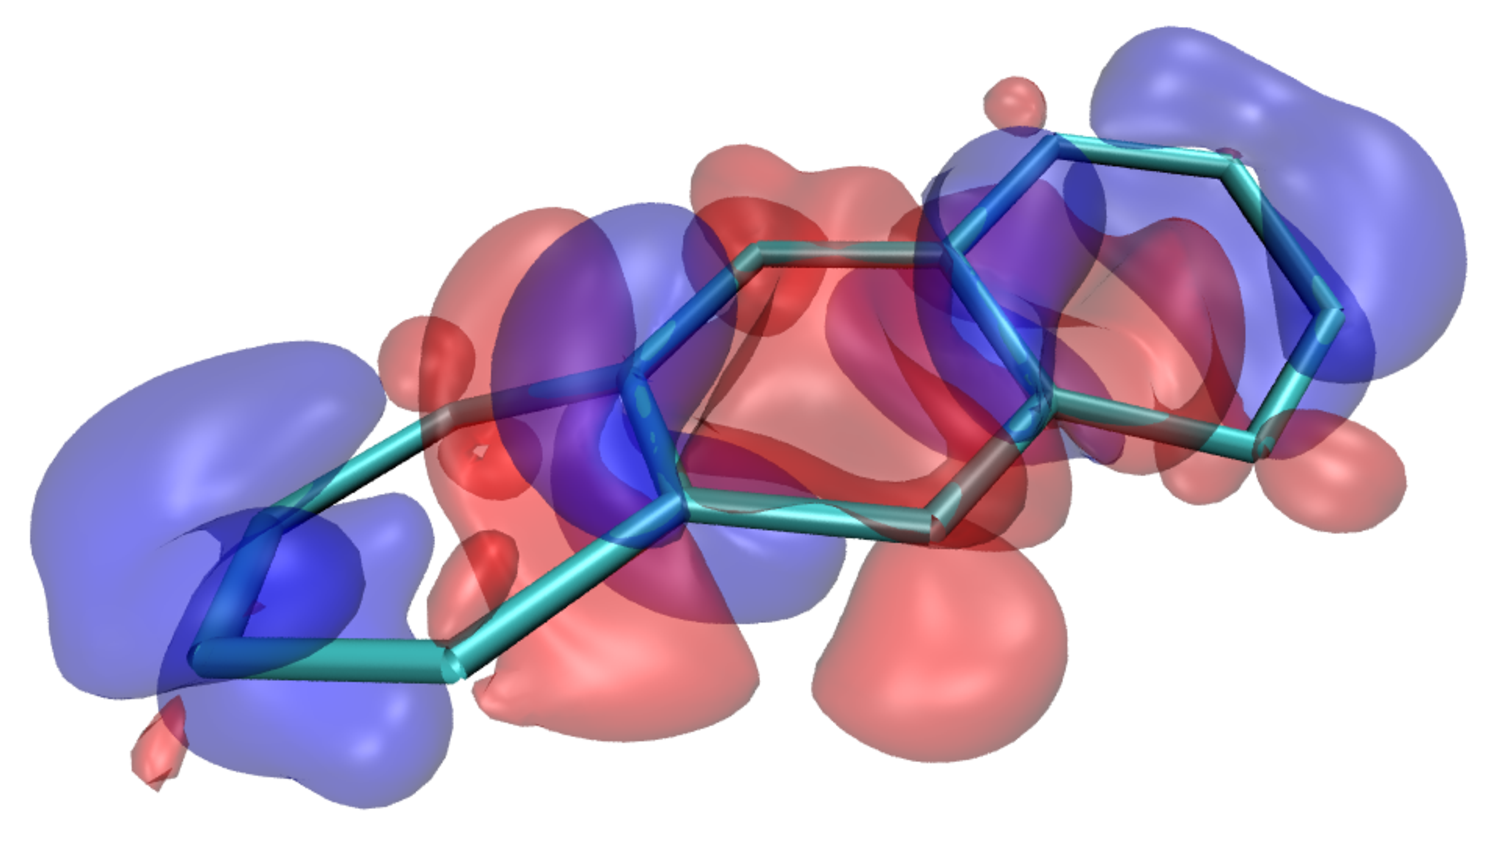
\includegraphics[width=4cm]{psc3-pk3} &
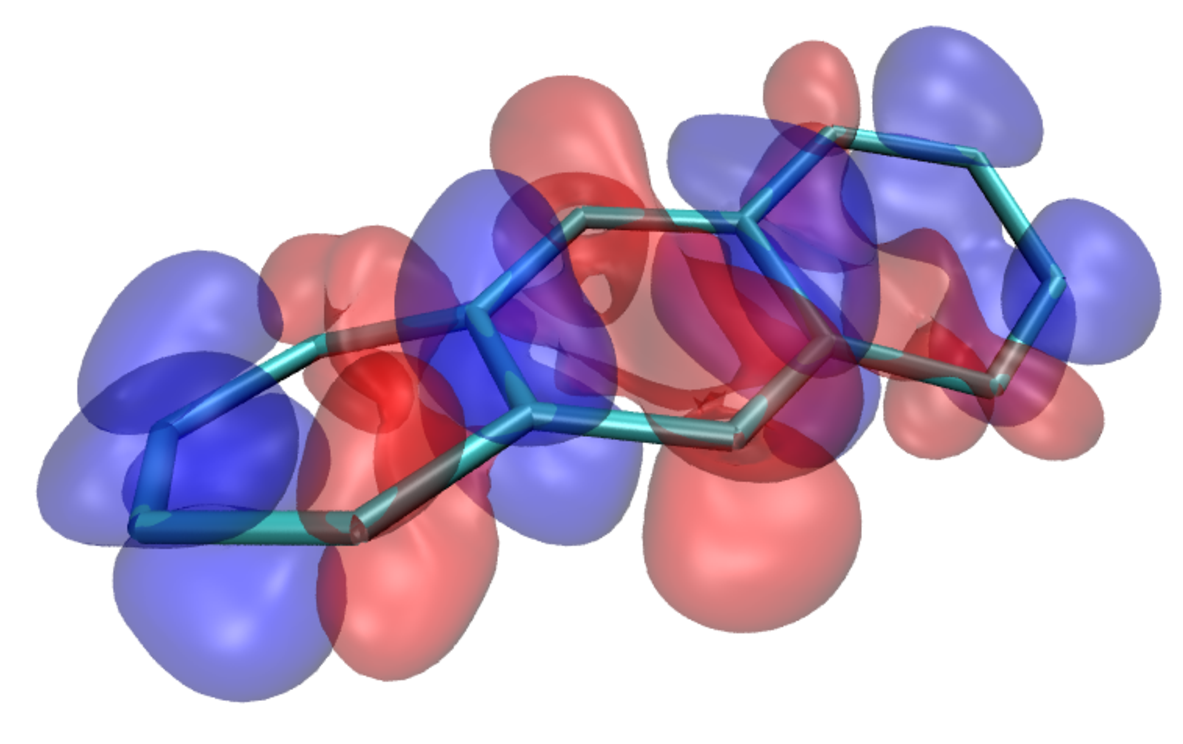
\includegraphics[width=4cm]{psc3-pk4} \\
(c) 215~$nm$ & (d) 225~$nm$ \\
\end{tabular}
\caption[Transition densities for pseudotwistacene.]{Transition densities for pseudoant-c3. Excitations from left to right, top to bottom: (a) 153~$nm$, (b) 177~$nm$, (c) 215~$nm$, (d) 225~$nm$. In each case, the charge transfer is from the blue regions to the red. These calculations are performed at the TDDFT-PBE0 level.}\label{fig:pstwistapeaks}
\end{figure}

Figure~\ref{fig:pstwistapeaks} displays transition densities for the five most distinct peaks in the pseudo-Ant-c3 ECD spectrum. We see immediately that in Figure~\ref{fig:pstwistapeaks}a the electron density is distorted in a mostly un-$\pi$-like manner, and so will not be physically representative of any transition present in the all-electron system. It is thought that Figures~\ref{fig:pstwistapeaks}b, c, and d might correspond to Figures~\ref{fig:twistapeaks}b, c, and d respectively. They are broadly $\pi$-like, although the shape of the electron densities do not correspond neatly to the respective all-electon densities in the way that the densities of transitions in the planar molecules do (see Appendix~\ref{app:edens}). One also notes a significant delocalisation across the central $\pi$ ring in all molecules, also observed in the [10]helicene densities of Section~\ref{sec:helicene}. The most distorted benzene rings in both [n]helicene and Ant-c$n$ are to be found in the centre of the molecules, and so we propose that the delocalisation of electron density toward the centre of the molecules, more strongly observed in the pseudomolecules than the all-electron molecules, is what is causing the distortion of the spectra, and that this extra delocalisation is caused by the extra distortion in the central rings, which makes the pseudopotentials a less accurate description of them.

In conclusion then, we can say that the pseudosystems were relatively successful at recreating the UV spectra of the distorted anthracene $\pi$ systems, up to and including a distortion of around 14.0$^{\circ}$ per benzene unit (Ant-c3), with the $geom_1$ potentials proving the most successful. However, even at the comparatively low rate of twisting of around 6.2$^{\circ}$ per benzene unit (Ant-c6), the pseudopotentials do not appear to be able to reproduce the ECD spectra of twistacene. This is in contrast to the helicene examined previously, where the pseudopotential ECD spectra were of good quality, despite in many cases a greater rate of planar distortion. We do not have a full explanation for this, but it seems to be in part a result of the nature of the particular excitations that dominate the spectra, and how much of a $\pi$ orbital character they have, as well as local planar distortion in regions of the molecule to and from which the charge transfer takes place.

\subsection{Complex Spectra: Dodecaphenyltetracene}
\label{sec:dodecaphenyltetracene}

In the process of searching through various acenes for suitable test molecules for the pseudopotentials (see Section~\ref{sec:twistacene}), we came across a recent synthesis of dodecaphenyltetracene~\cite{xiao_2019}. The complexity of this molecule, along with the fact the team had reported a UV spectrum to which theoretical spectra could be compared, made this an attractive challenge. The molecular structure is shown in Figure~\ref{fig:dodecaphenyltetracene}.

\begin{figure}
\begin{center}
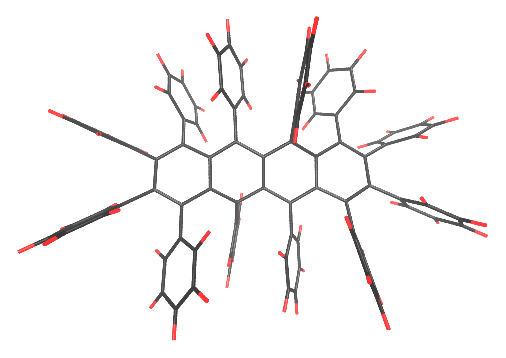
\includegraphics[width=8cm]{dodecaphenyltetracene}
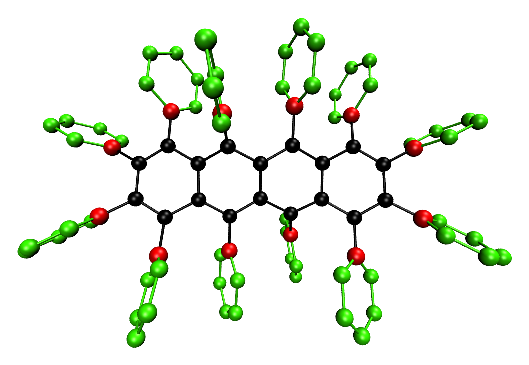
\includegraphics[width=8cm]{cc_psdodeca}
\caption[Dodecaphenyltetracene structure diagram.]{Dodecaphenyltetracene, with carbon in black and hydrogen in red (above). Pseudododecaphenyltetracene, with $\alpha$ pseudoatoms in green and $\beta$ pseudoatoms in red (below). All-electron atoms remain in black.}\label{fig:dodecaphenyltetracene}
\end{center}
\end{figure}

The reader will see that this molecule could encapsulate two different challenges. First are the phenyl groups, \emph{i.e.} the presence of many $\pi$ systems facing and overlapping one another at different angles. This is sure to involve the overlapping of many higher-energy orbitals, making for a complicated electronic structure. Second is the fact that the central tetracene is disorted by the phenyl groups. Since we already have both the twistacene  molecule in Section~\ref{sec:twistacene} and the helicene molecules in Section~\ref{sec:helicene} to investigate distorted $\pi$ systems, we decided to `pseudopotentialise' only the phenyl groups so as not to confuse the results. Figure~\ref{fig:dodecaphenyltetracene} shows the pseudomolecular system. This setup uses both $\alpha$ potentials, along with $\beta$ potentials connecting the phenyl rings to the central, all-electron tetracene.

\begin{figure}
\begin{center}
\includegraphics[width=8cm]{dodecaphenyltetracene_rpas.png}
\end{center}
\label{fig:dodecaphenyltetracene_spectra}
\caption[Dodecaphenyltetracene spectra: All-electron and pseudopotentials.]{UV spectrum of dodecaphenyltetracene using all-electron DFT-PBE0, as well as spectra using two different sets of pseudopotentials, also calculated at the DFT-PBE0 level.}
\end{figure}

At first glance the comparison of both pseudopotential spectra with the all-electron spectrum seems favourable. The $geom_1$ potentials show five clear peaks in near-agreement with the all-electron peaks, with the possible exception of the peak at around 300~$nm$ ($geom_1$) as compared to around 330~$nm$ (all-electron). The relative intensities of these peaks are also similar to those of the all-electron spectrum, althought they are somewhat skewed toward the lower-energy excitations by comparison. The $set4$ spectrum is more difficult to interpret. Despite containing excitations across roughly the same wavelengths and at rougly the same intensities as the all-electron spectrum, the peaks are not so clearly defined, with the exceptions of the peaks at 680~$nm$ and 360~$nm$. There is also a peak at 450~$nm$ that is not present in the all-electron spectrum.

The next comparison to be made is that of these theoretical results with the experimental ones in the original synthesis. The experimental spectrum extends from around 650~$nm$ to 250~$nm$ and has a spread of shallow excitations across the 600-450~$nm$ range, a clear and strong peak at 360~$nm$, and at least one further peak in the 250~$nm$ region. The stronger peaks (below 450~$nm$) are reproduced in the theoretical spectra, both in all-electron and pseudosystem calculations. The range of peaks between 600 and 400~$nm$ is not reproduced in any of the theoretical spectra. Comparison of theoretical and experimental spectra is complicated by the fact in the experimental results the molecules are in a CH$_2$Cl$_2$ solution.

Finally, we note that the HOMO energies of the all-electron system, the $geom_1$ and $set4$ systems are -4.941~$eV$, -5.476~$eV$ and -5.522~$eV$ respectively, making for percentage errors that are not dissimilar to those of the higher polyenes modelled previously (see Table~\ref{tab:set4_transpolyene_errors}).

In conclusion, these results for dodecaphenyltetracene show that this pseudopotential technique is effective at recreating the UV spectra of overlapping and interacting $\pi$ systems.

\subsection{Complex Spectra: Hemi-Cryptophane}

The interest in cryptophanes and hemicryptophanes lies in their propensity to form Van der Waals complexes as hosts. Some of these complexes have interesting catalytic properties~\cite{ikbal_2019}. The fact that their cavities and catalytic sites are lipophilic has led to an increasing interest in their use as biomimetics of enzymatic systems ~\cite{perraud_2013, gosse_2016}. 

Our own interest in such molecules is that they combine a range of different carbon environments with a complex electronic structure. This means we can test a variety of different pseudopotentials on the same molecule, as well as see how they perform in the presence of metal atoms. A further consideration is that such `cage molecules' are often characterised by their UV spectra, and so the ability to produce an accurate UV spectrum with a reduced pseudocage molecule would be useful practically.

The molecule we have adopted as a test subject is a Cu(II)hemicryptophane complex, shown in Figure~\ref{fig:cu2labellingscheme}. One can see that there are enough different chemical environments to test each kind of potential we have developed simultaneously. By creating a series of different 'pseudopotentialisations' of this molecule, we can build up an idea of what the pseudofragments can reproduce well, and where they fail, an idea of where the most chemically-sensitive parts of the molecule lie.

In order to try to make the investigation as systematic as possible, we decided to group parts of the molecule together as shown in Figure~\ref{fig:cu2labellingscheme}, before building up the number of pseudopotentials used. 

\begin{figure}
\begin{center}
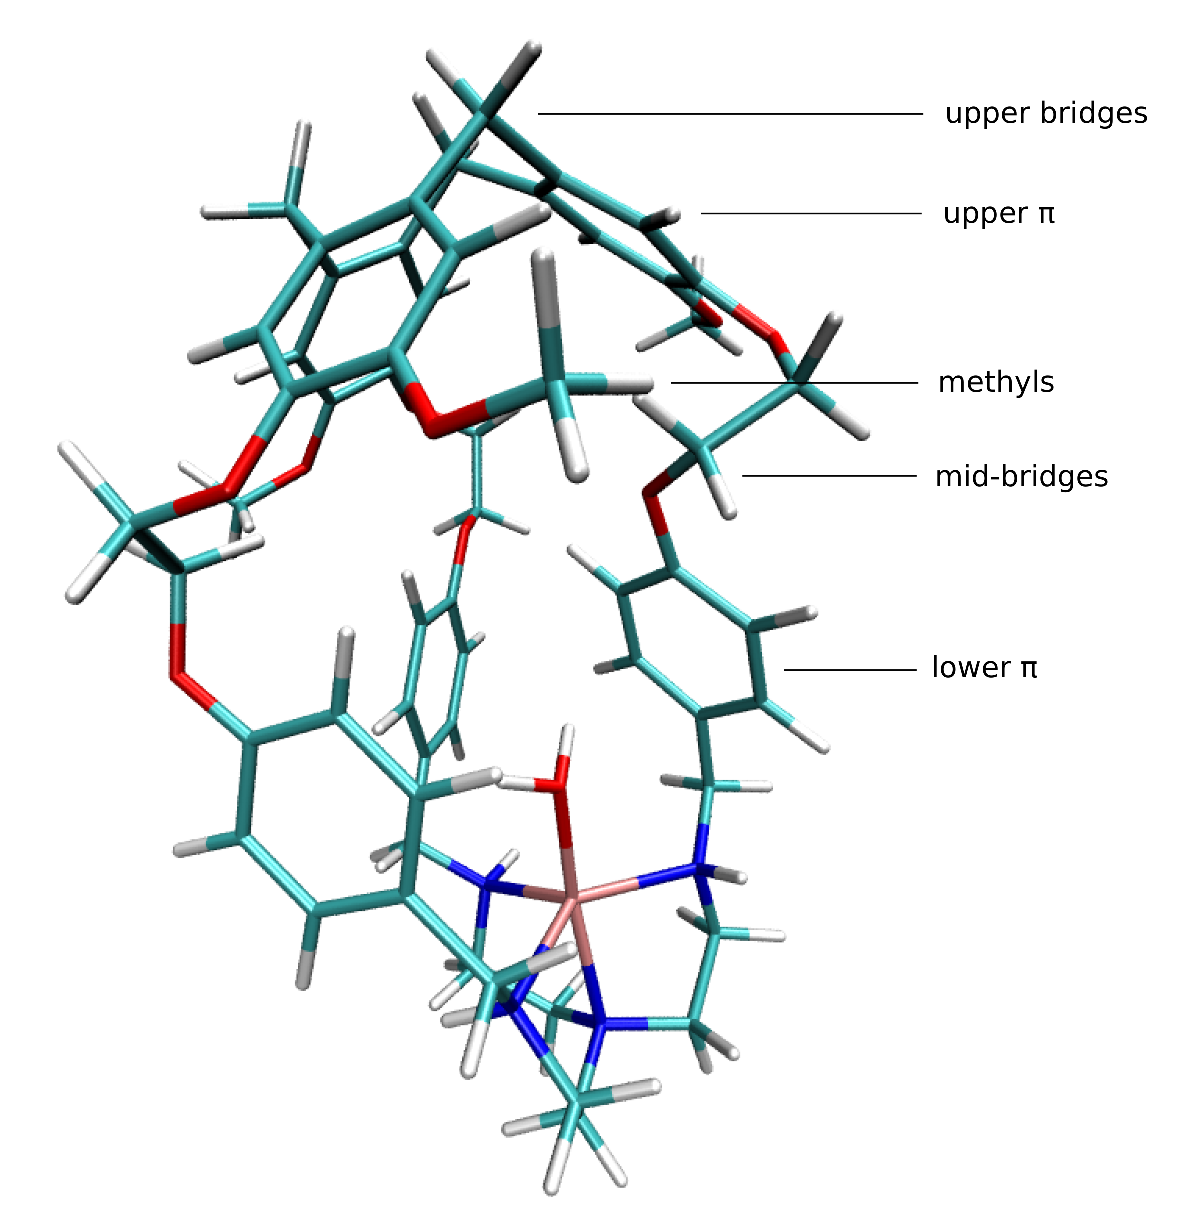
\includegraphics[width=8cm]{cagecubondslabels}
\caption{Labelling scheme for Cu(II)hemicryptophane complex,  where oxygen is in red, nitrogen in blue, and copper is pink.}\label{fig:cu2labellingscheme}
\end{center}
\end{figure}

In light of the results from Section~\ref{sec:simple_systems}, where we saw that the results were markedly less accurate when pseudogfragments were permitted to bond with heteroatoms, it was decide to institute a `no-heterobonding' rule for certain parts of certain pseudocomplexes, in order to see what the effects might be on the resulting spectra. An example of the `no-heterobonding' rule for the `upper $\pi$' section of the cage is shown in Figure~\ref{fig:cu2upperpi}. Figure~\ref{fig:cu2upperpi}a shows the regular-all-electron upper $\pi$ section of the cage. Figure~\ref{fig:cu2upperpi}b shows a version in which all carbon atoms have been replaced by pseudoatoms. Finally, Figure~\ref{fig:cu2upperpi}c shows the upper $\pi$ section following the no-heterobonding rule, in which there must be at least one all-electron carbon atom in between pseudogfragments and heteroatoms.

\begin{figure}
\begin{center}
\begin{tabular}{cc}
%\setatomsep{50pt}
\chemfig{
            % 9
     -[:180,.7]O% 8
     -[:120]% 2
     -[:180]% 1
               (
         -[:240]O% 7
         -[:240]R_1% 10
               )
    =_[:120]% 6
      -[:60]% 5
               (
         -[:130]% 11
         -[:90]R_2% 13
               )
          =_% 4
               (
          -[:50]% 12
          -[:90]R_3 % 14
               )
     -[:300]% 3
               (
        =_[:240]% -> 2
               )
} &
\chemfig{
              % 9
       -[:180,.7]O% 8
       -[:120]C^\ast_\beta% 2
       -[:180]C^\ast_\beta% 1
                 (
           -[:240]O% 7
       -[:240,,,1]R_1% 10
                 )
      =_[:120]C^\ast_\alpha% 6
    -[:60,,,1]C^\ast_\beta% 5
                 (
      -[:130,,1,1]% 11
      -[:90]R_2% 13
                 )
     =_[,,1,1]C^\ast_\beta% 4
                 (
       -[:50,,1,1]% 12
       -[:90]R_3 % 14
                 )
    -[:300,,1]C^\ast_\alpha% 3
                 (
          =_[:240,.7]% -> 2
                 )
} \\
\multicolumn{1}{c}{(a) all-electron system}
& \makecell{(b) pseudosystem \\ all-pseudoatom ring} \\
\multicolumn{2}{c}{\chemfig{
            % 9
     -[:180,.7]O% 8
     -[:120]% 2
     -[:180]% 1
               (
         -[:240]O% 7
         -[:240]R_1% 10
               )
    =_[:120]C^\ast_\beta% 6
      -[:60]C^\ast_\beta% 5
               (
         -[:130]% 11
         -[:90]R_2% 13
               )
          =C^\ast_\beta% 4
               (
          -[:50]% 12
          -[:90]R_3 % 14
               )
     -[:300]C^\ast_\beta% 3
               (
        =_[:240]% -> 2
               )
}} \\
\multicolumn{2}{c}{\makecell{ (c) pseudosystem \\ no-heterobonding rule}} \\
\end{tabular}
\caption{The `no heterobonding' rule for upper $\pi$ ring pseudopotentials.}
\label{fig:cu2upperpi}
\end{center}
\end{figure}

\begin{table}
\begin{center}
\caption[Breakdown of pseudoCu(II)hemicryptophane structures.]{Structures of pseudohemicryptophane  complexes. Each column represents a part of the molecule (see Figure~\ref{fig:cu2labellingscheme}) that has been replaced with potentials. The `heterobonding' column shows whether or not heterobonding has been permitted, \emph{i.e.} whether pseudofragments have been placed next to non-carbon atoms in the complex. For those systems with the `N ($\pi$)' designation, heterobonding is forbidden for carbons which are members of $\pi$ rings, but has been permitted elsewhere. The '\textasciitilde' symbol in the final column represents a molecule whose spectrum may contain neither, either or both peaks but which is distorted enough that we do not feel confident in assigning them.}
\label{tab:cu2comppots}
\begin{tabular}{|c|c|c|c|c|c|c|c|c|}
\hline
ID & \multicolumn{1}{m{1cm}|}{\centering upper $\pi$} & \multicolumn{1}{m{1.5cm}|}{\centering upper bridges} & methyls & mid-bridges & \multicolumn{1}{m{1cm}|}{\centering lower $\pi$} & heterobonding & Peaks \\
\hline
2 & Y & Y & Y & Y & N & Y & 2 \\ 
3 & Y & Y & N & N & N & N & 1, 2 \\
4 & Y & N & Y & N & N & Y & 2 \\
5 & Y & N & Y & N & N & N ($\pi$) & 1, 2 \\
6 & N & N & N & N & Y &  Y & \textasciitilde \\
3+5 & Y & Y & Y & N & N & N ($\pi$) & 1, 2 \\
7 & Y & N & Y & Y & N & N ($\pi$) & 1, 2 \\
8 & Y & Y & Y & Y & N & N ($\pi$) & 1, 2 \\
9 & Y & Y & Y & Y & Y & N ($\pi$) & \textasciitilde \\
\hline
\end{tabular}
\end{center}
\end{table}

Combining Figure~\ref{fig:cu2labellingscheme} with  Table~\ref{tab:cu2comppots} allows us to visualise each complex created with its different pseudopotentialisation scheme. If these are viewed alongside Figure~\ref{fig:cu2spectra} one can begin to see which parts of the molecule are responsible for producing the different parts of the spectra, and how well the pseudopotentials at each point have replicated the effects present in the all-electron system.

\begin{figure}
\begin{center}
\includegraphics[width=15cm]{cages_split}
\caption[All-electron and pseudoCu(II)hemicryptophane spectra.]{All-electron and pseudomolecular UV (above) and ECD (below) spectra for Cu(II)hemicryptophane. Calculations were carried out at the TDDFT-B3LYP level, with the first 20 singlet excitations.}\label{fig:cu2spectra}
\end{center}
\end{figure}

The reference spectra has two major features, a sharp, intense peak at around 800~$nm$ and a shallower and less intense peak centred at around 1900~$nm$. In the final column of Table~\ref{tab:cu2comppots}, these are labelled peaks 1 and 2, respectively. One thing that is immediately striking from Figure~\ref{fig:cu2spectra} is the range of different results. Since none of the pseudocomplexes uses any pseudopotentials below the `lower $\pi$' section of the molecule, we know therefore that a good part of the spectral activity of this molecule must arise from the hemicryptophane itself, and not just the metal ion and its immediate neighbours. This is hinted at in the original article, where electro-chemical studies revealed that the oxidation and reduction potentials of the complexes were dependent on the precise structure of the cage. What is revealed by pseudoresults however, is the magnitude of the effect of the `upper $\pi$' rings on the electronic structure. While most of the pseudocomplexes have replaced the `upper $\pi$' rings with pseudoatoms, only those which have respected the `no heterobonding' rule with respect to the $\pi$ atoms have been able to reproduce both peaks (pseudocomplexes 3, 5, 3+5 7, 8 and 9), whereas those which do not follow the no-heterobonding rule and have $\beta$ pseudopotentials bonded to the oxygens adjacent to the upper $\pi$ ring (that is, pseudocomplexes 2 and 4) are unable to reproduce peak 1. Furthermore, we see that structures which reproduce both peaks 1 and 2 have a much shallower peak 2 than the all-electron reference spectrum. These results tells us three things: 

\begin{enumerate}
\item A heteroatom bond (\emph{i.e.} a C-O bond) in the upper $\pi$ region of the molecule is largely responsible for peak 1. We can then compare pseudocomplex 3 (whose spectrum contains peak 1 and which has no pseudoatoms replacing the methyl groups) to pseudocomplex 5 (whose spectrum contains a near-identical peak 1 but does replace the methyl groups with pseudoatoms) to see that peak 1 must arise from the upper $\pi$ carbon-oxygen bond that connects to the mid-bridges (the oxygen bonded to R$_1$ in Figure~\ref{fig:cu2upperpi}). In the orginal article, this peak was attributed only to copper transitions, independent of the cage. Here we see the cage is in fact necessary for peak 1 to be produced.

\item Peak 2 has a strong upper $\pi$ component.
 
\item The difference between these results lies in the difference between the pseudopotentials used in the upper $\pi$ rings. The different structures of the upper $\pi$ ring pseudopotentials is diplayed in Figure~\ref{fig:cu2upperpi} for clarification. 
\end{enumerate}

Further to point 3, since we see that peak 2 is present in the all-electron spectrum (with upper $\pi$ rings as shown in Figure~\ref{fig:cu2upperpi}a), and also in the spectra 2 and 4 (with all-pseudopotential upper $\pi$ rings as in Figure~\ref{fig:cu2upperpi}b) and is also present but at a diminished intensity in spectra 3, 5, 7 and 8 and (with upper $\pi$ rings respecting the 'no-heterbonding' rule as shown in Figure~\ref{fig:cu2upperpi}c), this leads us to conclude that the reduced intensity of peak 2 is a result of the setup in Figure~\ref{fig:cu2upperpi}c reproducing the upper $\pi$ system less well than that in Figure~\ref{fig:cu2upperpi}b. 

Pseudocomplexes 6 and 9 are the only ones which have placed pseudopotentials on the lower $\pi$ rings of the molecule. The fact that spectrum 6 is shifted significantly from the reference spectrum, and that pseudocomplex spectrum 9 is shifted from pseudocomplex spectrum 8 (their respective counterparts with all-electron lower $\pi$ rings), suggests that delocalised electron density from the lower $\pi$ rings also contributes to the dominant excitations present in the spectra, though the fact that pseudocomplex 6 does not respect the heterobonding rule, and that pseudocomplex 9 has so many other pseudopotentials present in the system, makes it hard to draw conclusions. Further investigation would be needed to determine the exact nature of this effect.

The chirality of this molecule arises from the top of the hemicryptophane itself, and so one can expect to see the ECD spectra altered by the presence of the pseudopotentials. Looking at Figure~\ref{fig:cu2spectra}, this is indeed the case. Pleasingly, with the exception of pseudocomplexes 4 and 6, all the ECD spectra retain a clear postive-to-negative shift, \emph{i.e.} they are still obviously chiral. The most distinctive features of the all-electron system are a positive peak at around 800~$nm$, leading into a large, shallow negative peak at around 1900~$nm$. Pseudocomplex spectra 5, 3+5, 7, 8 and 9 broadly share these traits, albeit with intensities differing by up to a factor of around three. Pseudocomplex spectra 3 is somewhat distorted, and has no positive peak. The difference between pseudocomplex 3 and pseudocomplex 3+5 is in the pseudopotentialisation of the methyl groups. However, other pseudocomplexes which replace the methyl groups, e.g. 5, seem to reproduce this positive peak very well, and so it is hard to see the reason for the performance of pseudocomplex 3. Once more, the pseudocomplex spectra 6 and 9 appear shifted, and the pseudocomplex whose ECD spectrum matches best that of the all-electron calculation, in both wavelengths and intensities, is 3+5.

\begin{figure}
\begin{tabular}{c}
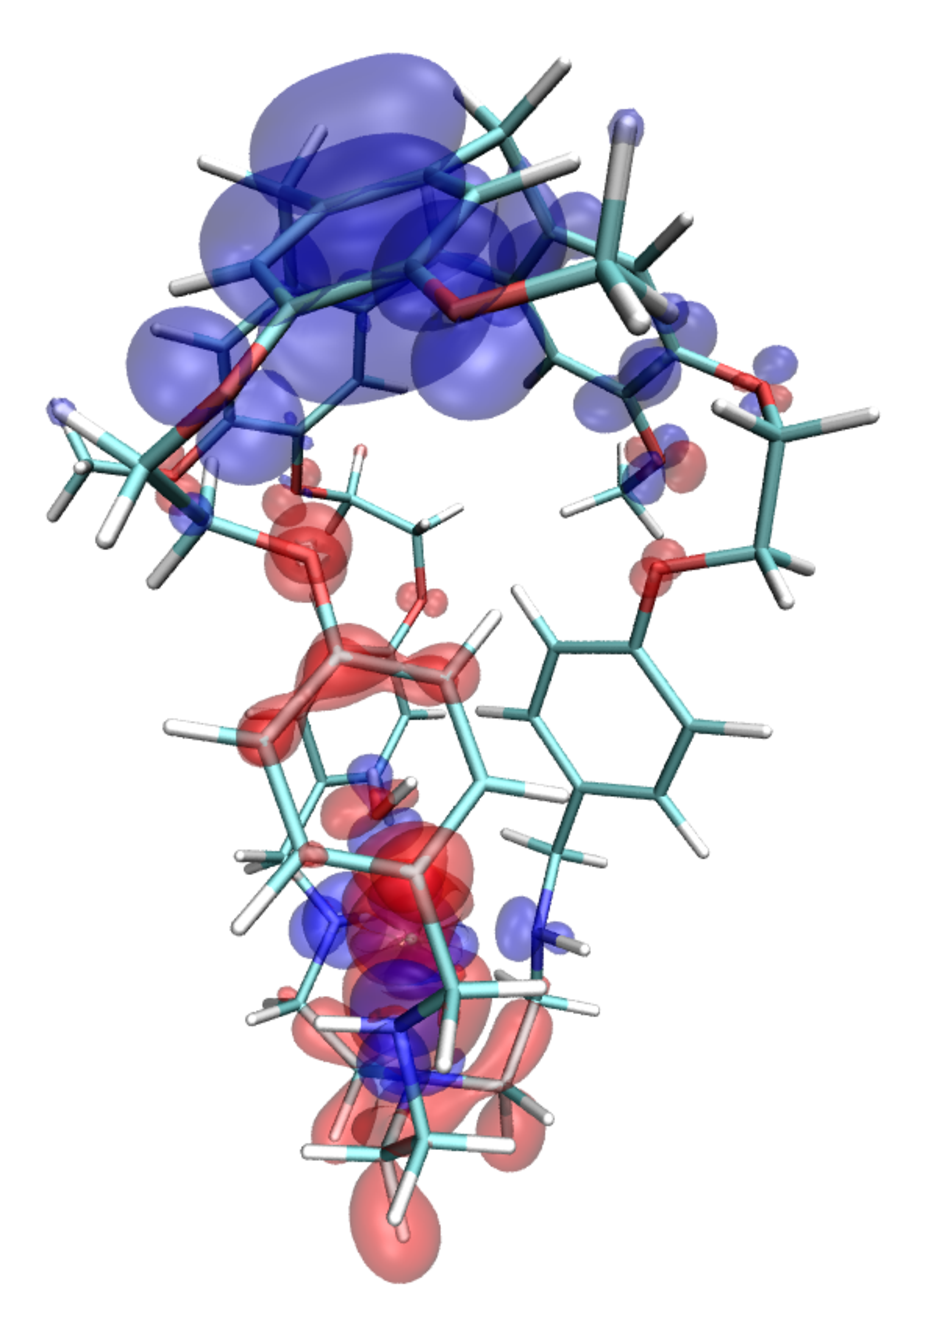
\includegraphics[width=8cm]{peak1} \\
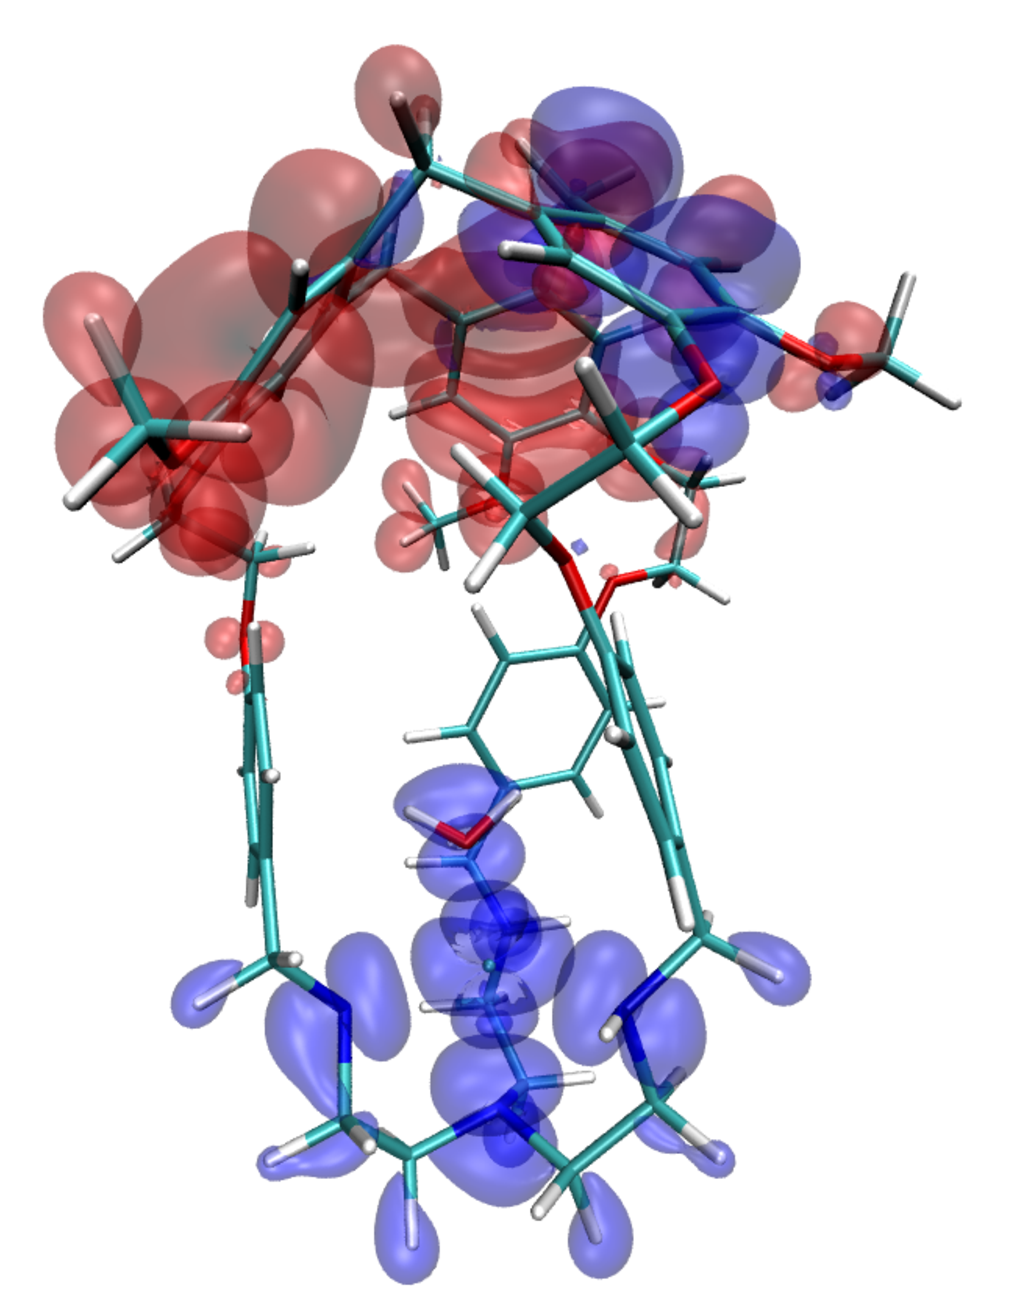
\includegraphics[width=8cm]{peak2}
\end{tabular}
\caption[Transition densities for Cu(II)hemicrytophane.]{Transition densities based on all-electron TDDFT-B3LYP calculations for excitation peaks 1 (left) and 2 (right). In both cases, electron density is reduced in the blue zones and increased in the red.}\label{fig:alletrdens}
\end{figure}

Figure~\ref{fig:alletrdens} displays the all-electron transition densities for peaks 1 and 2. These provide further evidence that deductions above regarding the nature of the two peaks are correct. Peak 1 broadly shows an electron transfer between upper and lower parts of the molecules, and the density on the upper part is indeed focused on the upper $\pi$ rings and the oxygen atoms directly below them. Peak 2 similarly contains a transfer of electron density between the top and bottom of the molecule, with a strong upper $\pi$ component.

We set out to replace as much of the hemicryptophane cage as possible with pseudopotentials, with the stipulation that the features of the UV and ECD spectra should still be identifiable. Many of the pseudocomplexes tested meet this criterion. The one which meets this criterion while removing the largest number of explicit electrons however, is pseudocomplex 8. From Table~\ref{tab:cu2comppots}, we see that this pseudocomplex applies the pseudopotentials from the upper bridges all the way down to the mid-bridges, while making sure to respect the no-heterobonding rule for the upper $\pi$ systems. This makes for an overall reduction in the number of explicit electrons in the complex of 132, from 545 to 413.

In conclusion then, this Cu(II)hemicryptophane complex is reproducible with simple carbon pseudopotentials, as we were able to recreate the key features of the complex's spectrum. This is particularly impressive given the heavy delocalisation of electron density over the whole molecule. However, it should be noted that it was necessary to derive a new rule in order to be sure of retaining the necessary electronic complexity, which is that bonds between pseudocarbons and all-electron atoms should be restricted to carbon-carbon bonds only, and that bonding pseudocarbons to explicit heteroatoms should be avoided. Given the results seen in Section~\ref{sec:simple_systems}, and given that all pseudocarbons in this work are optimised on carbon-carbon bonds, this seems reasonable.

%\subsection{Geometry Optimisation}
%
%Here go:
%
%\begin{itemize}
%\item geometry manipulation and optimisation of ethene (c-c distance, rotation curve, maybe graphs of fitting to gradient?)
%\item geometry manipulation and optimisation of ethane (c-c distance, rotation curve, maybe graphs of fitting to gradient?)
%\item geometry manipulation and optimisation of sp3 C*H*2 systems? I don't have all these results yet. Suggestions for tests so far:
%\begin{itemize}
%\item changing c-c distances/torsion of propane
%\item analysing acid dissociation (fluoroacetic for CH2, acetic for CH3?).
%\end{itemize}
%\item Attempts to find transferable potentials for C*H*(1,2,3)H(3,2,1), as well as whether these transfer to other systems.
%\end{itemize}


\section{Conclusion}

A glorious conclusion.

\section{Acknowledgments}
The authors acknowledge the french Ministère de l'éducation
nationale et de la recherche for providing the PhD grant of A. Punter.

\section{Supplementary materials}
In the supplementary materials are provided:
\begin{itemize}
\item Insightful material.
\end{itemize}

%%%%%%%%%%%%%%%%%%%%%%%%%%%%%%%%%%%%%%%%%%%%%%%%%%%%%%%%%%%%%%%%%%%%%%%%%%%%%%%%%
% BIBLIOGRAPHY

\bibliography{bibliography}   % Produces the bibliography via BibTeX.
\bibliographystyle{ieeetr} 

\end{document}

